\documentclass{article}
\usepackage{fullpage} % use entire page layout
\usepackage{times}     % smaller and better fonts that the standard latex ones
\usepackage[letterpaper]{geometry} % force letter format
\usepackage[colorlinks=true,linkcolor=black,urlcolor=blue,anchorcolor=black,citecolor=black,backref=none]{hyperref}
\usepackage[usenames,dvipsnames]{color}
%% Disable backref and make \href colors more decent:
\definecolor{MyDarkBlue}{rgb}{0,0.1,0.7}
\hypersetup{pdfborder={0 0 0},colorlinks,breaklinks=true,
  urlcolor={MyDarkBlue},citecolor={MyDarkBlue},linkcolor={MyDarkBlue} }
\newcommand{\ebookurl}{http://www.sigcomm.org/content/ebook}

\usepackage[absolute,showboxes]{textpos}

%set unit to be pagewidth and height, and increase inner margin of box
\setlength{\TPHorizModule}{\paperwidth}
\setlength{\TPVertModule}{\paperheight}
\TPMargin{5pt}

%define \copyrightstatement command for easier use
\newcommand{\copyrightstatement}{
    \begin{textblock}{0.65}(0.17,0.9)    % tweak here: {box width}(hposition, vposition)
         \noindent
         \footnotesize
         J. Cordero, J. Yi, T. Clausen, E. Baccelli ``Enabling Multihop Communication in Spontaneous Wireless Networks'', in H. Haddadi, O. Bonaventure (Eds.), \href{\ebookurl}{\emph{Recent
         Advances in Networking}}, (2013), pp. 413-457. Licensed under a
         \href{http://creativecommons.org/licenses/by-sa/3.0/}{CC-BY-SA}
         Creative Commons license. 
    \end{textblock}
}

\usepackage{graphicx}
\usepackage{amssymb}
\usepackage{amsmath}
\usepackage{multicol,multirow}
\usepackage{mdwlist}
\usepackage{epsf,pstricks}
\usepackage{rotating}
\usepackage{xspace}
\usepackage{url}
\usepackage{hyperref}
\urlstyle{rm}
\usepackage{capt-of}
\usepackage[ruled,vlined]{algorithm2e}
\usepackage[noend]{algpseudocode}
\usepackage{caption}
\usepackage{subcaption}


\newcommand{\martrace}{\textsf{MAR10}\xspace}
\newcommand{\btlong}{\textsf{BitTorrent-14d}\xspace}
\newcommand{\httplong}{\textsf{HTTP-14d}\xspace}
\newcommand{\dnslong}{\textsf{DNS-5d}\xspace}
\newcommand{\cate}{\textsf{CaTE}\xspace}
\newcommand{\epsfrag}[2]{\psfrag{#1}[cc][cc]{\fontsize{6}{5}\selectfont \sffamily #2}}
\newcommand{\epsfragl}[2]{\psfrag{#1}[lc][lc]{\fontsize{6}{5}\selectfont \sffamily #2}}
\newcommand{\padis}{\textsf{PaDIS}\xspace}
\newcommand{\MDC}{{Microdatacenter}\xspace}
\newcommand{\MDCs}{{Microdatacenters}\xspace}
\newcommand{\Netpaas}{{NetPaaS}\xspace}
\newcommand{\ONSERVICE}{{ON-DEMAND SERVICE}\xspace}
\newcommand{\OnService}{{On-Demand Service}\xspace}
\newcommand{\Onservice}{{On-demand service}\xspace}
\newcommand{\onservice}{{on-demand service}\xspace}
\newcommand{\Ondemandbase}{{On-demand service deployment}\xspace}
\newcommand{\ondemandbase}{{on-demand service deployment}\xspace}
\newcommand{\onserviceemph}{\emph{on-demand service}\xspace}
\newcommand{\sliceallocation}{\texttt{slice lo\-ca\-tion}\xspace}
\newcommand{\sliceassignment}{\texttt{user-slice as\-sign\-ment}\xspace}

%%%
%%% Figure stuff
%%%
\renewcommand{\topfraction}{1}
\renewcommand{\dbltopfraction}{1}
\renewcommand{\floatpagefraction}{1}
\renewcommand{\dblfloatpagefraction}{1}
\renewcommand{\textfraction}{0}
%\renewcommand{\baselinestretch}{.985}

%%
%% General definitions one needs all the time
%%

\newcommand{\nibp}{\noindent\hspace{0.3em}\textbullet\hspace{0.7em}}

\newcommand{\xref}[1]{Section~\ref{#1}}
%\newcommand{\xref}[1]{\S\ref{#1}}
\newcommand{\cref}[1]{Chapter~\ref{#1}}
\newcommand{\pxref}[1]{(\xref{#1})}
\newcommand{\fref}[1]{Figure~\ref{#1}}
\newcommand{\tref}[1]{Table~\ref{#1}}
\newcommand{\see}[1]{~(see \xref{#1})}
\newcommand{\first}{\emph{(i)}~}
\newcommand{\second}{\emph{(ii)}~}
\newcommand{\third}{\emph{(iii)}~}
\newcommand{\fourth}{\emph{(iv)}~}
\newcommand{\fifth}{\emph{(v)}~}
\newcommand{\sixth}{\emph{(iv)}~}

\newcommand{\zb}{z.B. \@}

\newcommand{\ie}{i.e., \@}
\newcommand{\eg}{e.g., \@}
\newcommand{\etc}{etc., \@}
\newcommand{\Ie}{I.e., \@}
\newcommand{\Eg}{E.g., \@}
\newcommand{\cf}{cf. \@}
\newcommand{\Cf}{Cf. \@}

\newcommand{\etal}{et~al.\xspace}

\newcommand{\perc}{\,\%\xspace}
\newcommand{\pert}{\,\textperthousand\xspace}


\newcommand{\checked}{\ding{52}\xspace}
\newcommand{\unchecked}{\ding{56}\xspace}

\newcommand{\osonly}{\textsf{OS only}\xspace}
\newcommand{\osbrow}{\textsf{OS + browser version}\xspace}

\newcommand{\lstfun}[1]{function \lstinline[basicstyle=\normalsize]{#1}\xspace}
\newcommand{\lstfuns}[2]{functions \lstinline[basicstyle=\normalsize]{#1} and \lstinline[basicstyle=\normalsize]{#2}\xspace}

% "smallitemize"-environment like "itemize" but more dense
\newenvironment{smallitemize}{%
\begin{itemize}%
\setlength{\parsep}{0.3ex}%
%\setlength{\itemindent}{-3ex}%
\setlength{\leftmargin}{0.1pt}%
\setlength{\listparindent}{-8ex}%
\setlength{\itemsep}{0.2ex}%
\setlength{\topsep}{0ex}%
\setlength{\parskip}{0ex}%
\setlength{\partopsep}{0ex}%
}{%
\end{itemize}
}%

% "smallenumerate"-environment like "enumerate" but more dense
\newenvironment{smallenumerate}{%
\begin{enumerate}%
\setlength{\parsep}{0.3ex}%
%\setlength{\itemindent}{-3ex}%
\setlength{\leftmargin}{0.1pt}%
\setlength{\listparindent}{-8ex}%
\setlength{\itemsep}{0.2ex}%
\setlength{\topsep}{0ex}%
\setlength{\parskip}{0ex}%
\setlength{\partopsep}{0ex}%
}{%
\end{enumerate}
}%


\newcommand{\todo}[1]{\textit{\textcolor{red}{TODO: #1}}}
\newcommand{\anja}[1]{\textit{Anja: #1}}
\newcommand{\georgios}[1]{\textit{\textcolor{green}{George: #1}}}
\newcommand{\ingmar}[1]{\textit{\textcolor{blue}{Ingmar: #1}}}
\newcommand{\ben}[1]{\textit{\textcolor{brown}{Benjamin: #1}}}
\newcommand{\steve}[1]{\textit{\textcolor{orange}{Steve: #1}}}

%\renewcommand{\todo}[1]{}

% mark changed wording from first submission
\newcommand{\new}[1]{\textcolor{blue}{#1}}
\newcommand{\discuss}[1]{\textit{\textcolor{green}{Discuss: #1}}}

%\definecolor{mygrey}{rgb}{0.8,0.8,0.8}

\newcounter{fn1}
\setcounter{fn1}{1}
\newcounter{fn2}
\setcounter{fn2}{2}
\newcounter{fn3}
\setcounter{fn3}{3}
\newcounter{fn4}
\setcounter{fn4}{4}
\newcounter{fn5}
\setcounter{fn5}{5}
\newcommand{\fnsym}[1]{$^{\fnsymbol{#1}}$}

\newcommand{\minisec}[1]{\noindent\textbf{#1}:}

%%%
%%% Definitions specific to some papers
%%%

\newcommand{\libpcap}{\textsc{libpcap}\xspace}
\newcommand{\winpcap}{\textsc{winpcap}\xspace}
\newcommand{\libz}{\textsc{libz}\xspace}
\newcommand{\tcpdump}{\textsc{tcpdump}\xspace}
\newcommand{\snort}{\textsc{snort}\xspace}
\newcommand{\ipsumdump}{\textsc{ipsumdump}\xspace}
\newcommand{\wireshark}{\textsc{Wireshark}\xspace}
\newcommand{\bro}{\textsc{Bro}\xspace}
\newcommand{\spbc}{\textsc{spbc}\xspace}

\newcommand{\capname}{FIX ME}
\newcommand{\capcomment}{\small \mdseries}
\renewcommand{\capname}{ \xspace}



\def\N{{\sf I\hspace*{-1pt}N}}
\def\R{{\sf I\hspace*{-1pt}R}}


\def\QEDclosed{\mbox{\rule[0pt]{1.3ex}{1.3ex}}} % for a filled box
\def\QEDopen{{\setlength{\fboxsep}{0pt}\setlength{\fboxrule}{0.2pt}\fbox{\rule[0pt]{0pt}{1.3ex}\rule[0pt]{1.3ex}{0pt}}}}
\def\QED{\QEDclosed} % default to closed
\def\proof{\noindent\hspace{2em}{\itshape Proof: }}
\def\endproof{\hspace*{\fill}~\QED\par\endtrivlist\unskip}
%
\newtheorem{Definition}{Definition}
%
\begin{document}

\title{Collaboration Opportunities for\\Content Delivery and Network Infrastructures}


\author{
Benjamin~Frank, Ingmar~Poese, \href{http://www.smaragdakis.net/}{Georgios~Smaragdakis},\\
\href{http://www.net.t-labs.tu-berlin.de/~anja/}{Anja~Feldmann}, \href{http://www.cs.duke.edu/~bmm/}{Bruce M. Maggs},  \href{http://www.eecs.qmul.ac.uk/~steve/}{Steve~Uhlig},\\
Vinay~Aggarwal, and Fabian~Schneider
}
\date{}

\copyrightstatement

\pagestyle{empty}

\maketitle

\thispagestyle{empty}

%
%\tableofcontents
%
%\newpage 
\section{Motivation}

The Internet is a hugely successful man-made artifact that has changed society
fundamentally.  Imagine the effect a prolonged outage of the Internet would
have: (1) Youngsters wouldn't know how to interact with their peers and how to
spend their leisure time as they increasingly rely on social networks, online
games, YouTube, and other online entertainment offerings.  (2) Manufacturing
would hit a roadblock as the communication paths within and between companies
increasingly rely on the Internet. (3) Control of critical infrastructures
would be hampered as it increasingly relies on the Internet for gathering input
data and propagating control information.

In becoming a hugely successful infrastructure, the usage of the Internet and
thus its structure has also undergone continuous changes. Usage has changed
from dominance by email and FTP in the early days, to the World Wide Web (WWW)
from 1995 to 2000, to peer-to-peer applications (P2P) from 2000 to 2007, back
to the WWW since 2007. These changes are driven in part by the Internet users'
interests as well as how content, including user generated content, is made
available.

When considering the current application mix and traffic streams in the
Internet, the latest buzz is that ``Content is King'' just as Bill
Gates~\cite{Gates-Content-King} predicted in his essay from 1996.  Hereby, the
term content has to be seen very broadly and encompasses everything from
commercially prepared content, \eg broadcast and interactive TV, news, and
software, to user-generated content, \eg videos uploaded to YouTube, and photos
uploaded to Flickr, to interactive activities, \eg online games. Or to quote
Bronfman~\cite{Bronfman-remarks}, the head of a major music producer and
distributor: ``What would the Internet be without `content'? It would be a
valueless collection of silent machines with gray screens. It would be the
electronic equivalent of a marine desert---lovely elements, nice colors, no
life.  It would be nothing.''

The idea of content delivery being the fundamental operation around which to
design future Internet architecture for comes as no surprise. In fact, the idea
of Content-Centric Networking (CCN)~\cite{CCN} is guided by this principle.
Change, however, takes time, and when hundreds of million of devices are
involved, change can only be made slowly. Before such a novel and radically
different architecture such as CCN is available or potentially deployable, the
Internet in its current state must cope with the challenge of delivering
ever-increasing amounts of content to Internet users.

Accordingly, it appears that solely providing connectivity to end users is no
longer sufficient for Internet Service Providers (ISPs).  Yet, connectivity is
a crucial ingredient and some authors, \eg Andrew
Odlyzko~\cite{odlyzko2001content} have opined that enabling communication is
the main task of the Internet network infrastructure. In his paper ``Content is
not king'' he claims that ``Content will have a place on the Internet, possibly
a substantial place. However, its place will likely be subordinate to that of
business and personal communication''.

At this point it is crucial to realize that the producers of content are
usually not the operators of today's Internet infrastructure. Nonetheless, both
content producers and network operators depend on each other. In fact, neither
the Internet infrastructure operators nor the content producers can be
successful without the other.  After all, the content producers want to ensure
that their content gets to Internet users with reasonable performance for which
they need to rely on the network infrastructure.  On the other hand, the
network infrastructure providers have to transport the content and manage the
infrastructure to satisfy the demand for content from their subscribers. It is
this symbiosis between the two parties that motivates our work collaboration
between content producers and network operators in delivering content.

\bigskip 

\noindent\textbf{Outline:} We start this chapter with a short introduction in
Section~\ref{sec:introduction}.  Then, in Section~\ref{sec:ISP}, we set the
stage by providing an overview of today's Internet network infrastructure,
discussing how Internet Service Providers (ISPs) perform traffic engineering,
and reviewing the Domain Name System (DNS), an essential component of any
Web-based content-delivery architecture.   Next, we review current trends in
Internet traffic and the application mix as well as traffic dynamics in
Sections~\ref{sec:traffic} and~\ref{sec:traffic-diversity}.

We finish the overview with a brief summary on the background of content
delivery in Section~\ref{sec:overview}. Here, we assume that the reader is
familiar with the basic architecture of the Web. There are excellent text books
on this topic, \eg~\cite{web-book}.  Given that there are several approaches to
content delivery, we provide a general high level description of how different
Content Delivery Infrastructures work.  Since there are also many peer-to-peer
based content delivery systems we provide a short review of the basic P2P
architectures as well. For additional background on P2P we refer the reader to,
\eg~\cite{p2pbook1,p2pbook2}.

An overview of the current content delivery spectrum is presented in
Section~\ref{sec:content-delivery}. Here we discuss various types of Content
Delivery Infrastructures (CDIs) which range from Web-based Content Distribution
Networks (CDNs) to Hybrid CDNs to peer-to-peer (P2P) systems. Furthermore, in
Section~\ref{sec:challenges} we turn to the challenges that each party involved
in Internet content delivery faces separately today.

Finally, we turn to the state of the art of collaboration between networks and
content providers.  We start by outlining the collaboration incentives for each
member of the content delivery landscape in Section~\ref{sec:Incentives}. Next
we review the collaboration schemes that have been discussed in research as
well as at the Internet Engineering Task Force (IETF) in
Section~\ref{sec:Opportunities}. We briefly introduce the well-known approaches
and summarize their key functions. We then pick two collaboration schemes,
namely the P2P Oracle and the Provider-aided Distance Information System
(PaDIS) for a case study. In Section~\ref{sec:oracle} we discuss the P2P Oracle
with regards to its effect on the P2P system as well as on network operations.
Likewise, the second case study discusses the model of the Provider-aided
Distance Information System in Section~\ref{sec:te-cate}, including a large
scale analysis based on real traffic traces.  Section~\ref{sec:future} outlines
a possible future direction for collaboration between content providers and
network operators.  We conclude this part of the chapter in
Section~\ref{sec:conclusion}.


\bigskip 

\noindent\textbf{Summary:} This chapter builds upon the student's
basic knowledge of how the Internet infrastructure operates, i.e., as a network
of networks. After reading this chapter the student should have a fundamental
understanding about how content distribution via the Internet works today, what
the challenges are, and which opportunities lie ahead. Moreover, the chapter
points out how all parties---including end users---can benefit from the
collaboration between ISPs and content providers. Indeed, simple, almost
intuitive, means will enable such collaboration.

%
%\newpage
%%%%%%%%%%%%%%%%%%%%%%%%%%%%%%%
\section{Introduction}\label{sec:introduction}
%%%%%%%%%%%%%%%%%%%%%%%%%%%%%%%

Recent traffic studies~\cite{TrafficTypesGrowth:2011,arbor,PADIS2010} show that
a large fraction of Internet traffic is due to content delivery and is
originated by a small number of Content Delivery Infrastructures (CDIs). Major
CDIs include highly popular rich-media sites like YouTube and Netflix,
One-Click Hosters (OCHs), \eg RapidShare~\cite{OCH-performance},
Content Delivery Networks (CDNs) such as Akamai and Limelight, and
hyper-giants, \eg Google, Yahoo!, and Microsoft.  Gerber and Doverspike~\cite
{TrafficTypesGrowth:2011} report that a few CDIs account for more than half of
the traffic of a US-based Tier-1 carrier.  Poese \etal~\cite{PADIS2010} report
a similar observation from the traffic of a European Tier-1 carrier. Labovitz
\etal~\cite{arbor} infer that more than 10\% of the total Internet inter-domain
traffic originates from Google, and Akamai claims to deliver more than 20\% of
the total Internet Web traffic~\cite{Akamai-Network}. Netflix alone, a company
that offers a high definition video video-on-demand streaming service, is
responsible for a significant fraction of the traffic in North America ISPs
during peak hours~\cite{sandvine,Netflix-CDN-presentation}.

To cope with the increasing demand for content, CDIs have deployed massively
distributed server infrastructures to replicate content and make it accessible
from different locations on the Internet \cite{CDNsec2009}. These
infrastructures have multiple choices as to how and where to place their
servers. As described in~\cite {ImprovingPerformanceInternet2009}, the main
approaches are (1) centralized hosting, (2) data center-based CDIs, (3)
edge-cache-based CDIs, and (4) peer-to-peer (P2P) networks. Approaches~2 and~3
scale content delivery by distributing the content onto dedicated
infrastructures.  These infrastructures can be composed of a few large data
centers, a large number of edge caches, or any combination thereof.

To complicate matters further, some of these infrastructures are entangled with
the very infrastructures that provide network connectivity to end-users. For
example, one of the largest players in content delivery, Akamai, operates more
than 120,000 servers in more than 2,000 locations across nearly 1,150 ISP
networks~\cite {Akamai-Network,Akamai-website}. Google is reported to operate
tens of data centers and front-end server clusters
worldwide~\cite{MovingBeyondE2E2009,Tariq:What-if,Google-Datacenters}.
Microsoft has deployed its content delivery infrastructure in 24 locations
around the world~\cite{azure}. Amazon maintains at least 5 large data centers
and caches in at least 21 locations around the world~\cite{amazon}. Limelight
operates thousands of servers in more than 22 delivery centers and connects
directly to 600 networks worldwide~\cite{LLNetworks}. Last but not least, P2P
networks rely on a huge number of end users to store, replicate, and distribute
content.

Despite the significant entanglement between the infrastructures that deliver
content and the network connectivity fabric, our knowledge of their
interactions is largely through the literature on network interconnections, \eg
see the recent book by W. Norton~\cite{peering-playbook}. Given the nature of
network interconnections, previous work has studied the interactions from an
economic perspective~\cite
{internet-economics,interactions-economics,content-oriented-economics}. The
limited knowledge available about the settlements between networks have led
researchers to try to reason about why peering choices are made~\cite
{ToPeerOrNot:Infocom2006} and what drives the evolution of the
Internet~\cite{evolution}.

Most of the literature has considered the interactions between content and the
network indirectly, \eg through peerings and traffic measurements, despite
recent changes in Internet traffic~\cite{TrafficTypesGrowth:2011,arbor} that
have shown the importance of content and applications.  The observed changes in
traffic, either through direct traffic measurements~\cite
{TrafficDemand:ToN2001,Feldmann:Kammenhuber:2004,uhlig-public,arbor,IXPSIGCOMM2012},
or through
inference~\cite{medina_tm:2002,zhang_tm:2003,zhang_link:2003,gunnar_estimation:2004,dina_distributed:2004,soule_tm:2005}
have repeatedly shown how volatile traffic can be. With the rise of
user-generated content and large shifts in content popularity, traffic
volatility has become especially relevant.

Handling changes in traffic has traditionally been done through traffic
engineering (TE). Initially, traffic engineering was used by large network
operators to optimize the utilization of their networks
\cite{Awduche_OverviewTE:2002}. The vast majority of the traffic engineering
literature has therefore focused on traffic engineering inside a single network
\cite{netscope,FT00,Xiao_Traffic:2000,Aukia_RATES:2000,MPLS:Infocom2000,FT01}.
In reality, most of the traffic in the Internet is exchanged between different
networks \cite{arbor}, and especially directly between data centers and
residential ISPs \cite{IXPSIGCOMM2012}. Organizations that originate a lot of
content, \eg Google, connect directly to a large number of other networks
\cite{arbor}, and need to optimize how content leaves their networks.
Organizations that provide Internet access to broadband or mobile users
typically wish to optimize how traffic enters their networks, as most users
still download more content than they upload. In between, transit ISPs try to
balance the load of the traffic exchanged between the networks they connect.

Traditional traffic engineering aims at reducing the likelihood that
bottlenecks arise inside a given network due to mismatches between network
provisioning and expected demand. Changes in network provisioning are slow,
taking place over time scales of weeks or months. Popular content, on the other
hand, generates bursts in demand over much smaller time scales, \eg hours or
minutes. Today's Internet requires much more reactive network control
techniques than those we have today, and these techniques must take content
delivery into consideration. A few steps have been made in this direction.
Indeed, collaborative approaches
\cite{TECDN,CooperativeSettlement:ToN,Cate-CCR} have been proposed to help deal
with the traffic generated by content delivery infrastructures. Even in the
case of P2P, portals have been proposed to allow P2P applications and users to
communicate with ISPs to receive updated views of their networks~\cite{p4p}. In
broad terms, all information CDIs are missing today for optimizing their
operations is available to ISPs. Combined with the already proposed schemes for
collaboration, it is surprising how little real collaboration is performed in
today's Internet between these parties.

In this chapter, we analyze the operation of CDIs as well as network operators.
The analysis demonstrates the potential for fruitful collaboration.  We argue
that for collaboration to become more common, it is important for every party
in the content delivery landscape, \ie the content delivery infrastructures,
the network operators, and the end users, to benefit.  Finally, we present, in
depth, two systems that have incentives for every party and that can readily be
used today.


%
%\newpage
%%%%%%%%%%%%%%%%%%%%%%%
\section{Internet Network Infrastructure}\label{sec:ISP}
%%%%%%%%%%%%%%%%%%%%%%%

\begin{figure*}
  \begin{center}
  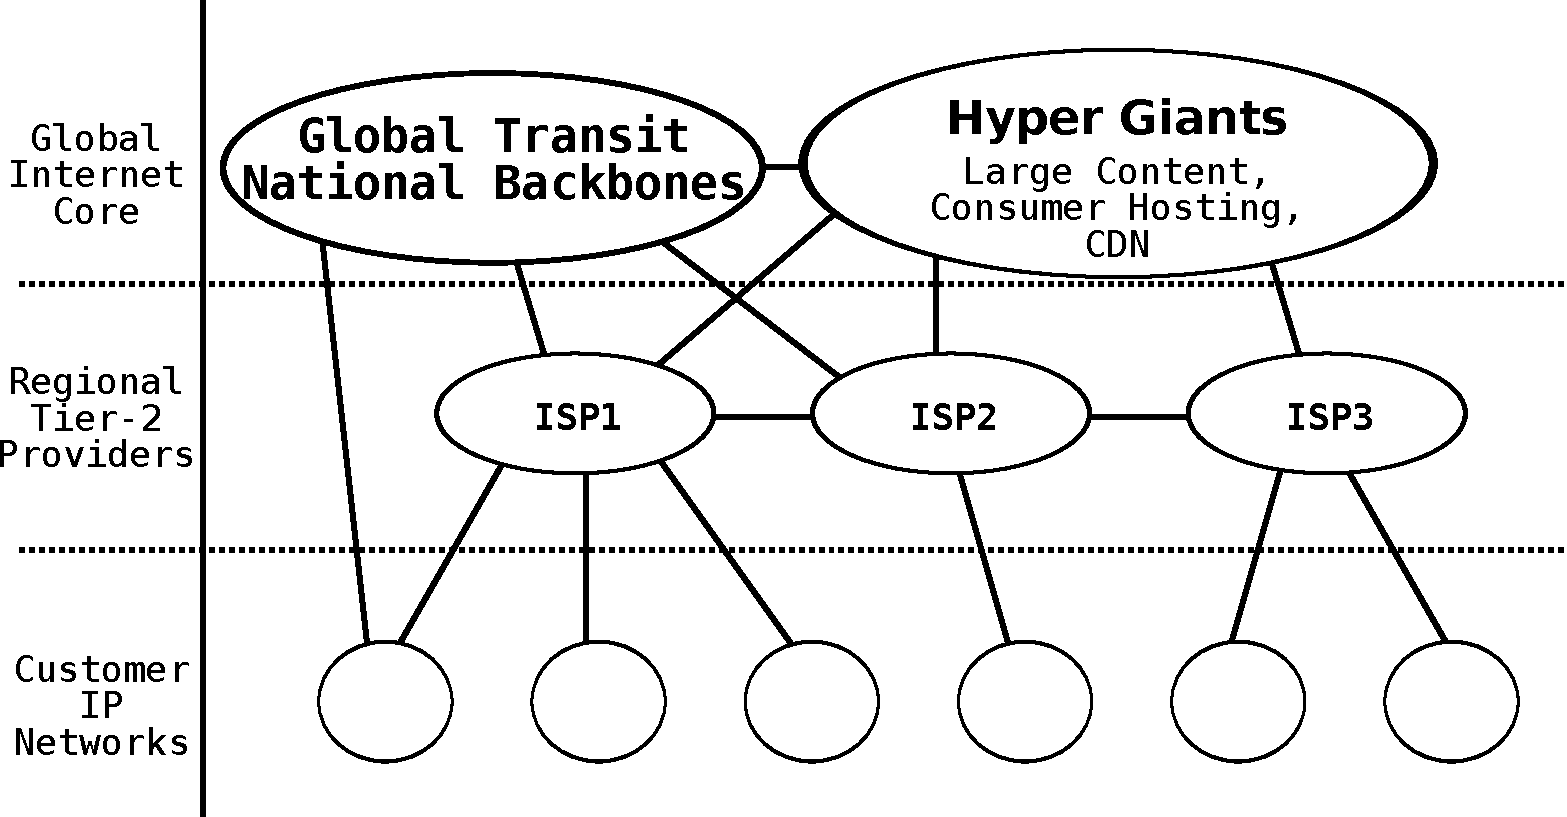
\includegraphics[width=\linewidth]{figures-pdf/Internet-Layout}
  \end{center}
  \caption{Layout of the Internet Structure }
  \label{fig:InternetLayout}
\end{figure*}

The Internet Network Infrastructure is provided by a set of Internet Service
Providers (ISPs).  An ISP is, in general terms, an organization that provides
access to the Internet for its customers.  The Internet is structured by the
interconnection of multiple individual networks run by ISPs.  However, control
of an individual network remains solely with the ISP operating it. Figure~\ref
{fig:InternetLayout} shows how the Internet is structured today~\cite{arbor}.
Here, the ISPs run their own networks. This forces a clear distinction between
the individual network that an ISP runs and the global Internet as a network of
networks.  Also, from this, it can be deduced that nobody has control over the
Internet, but instead each ISP has only control over its own network and the
direct connections to other networks.


To be able to interconnect with other networks, an ISP needs to operate an
autonomous system (AS). An AS is an administrating entity, generally under the
control of one administrative domain. On the technical side, each AS is usually
managed by an Interior Gateway Protocol (IGP), \eg OSPF~\cite{RFC2328} or
ISIS~\cite{RFC1142} while the Border Gateway Protocol (BGP~\cite{RFC4271}) is
the de-facto standard for interconnecting different ASes. For more information
and additional details about the Internet topology, we'd like to refer the
reader to Chapter 7 of this book~\cite{ebook-chapter7-Redux}.


\subsection{Traffic Engineering in an AS}

\begin{figure} \begin{center}
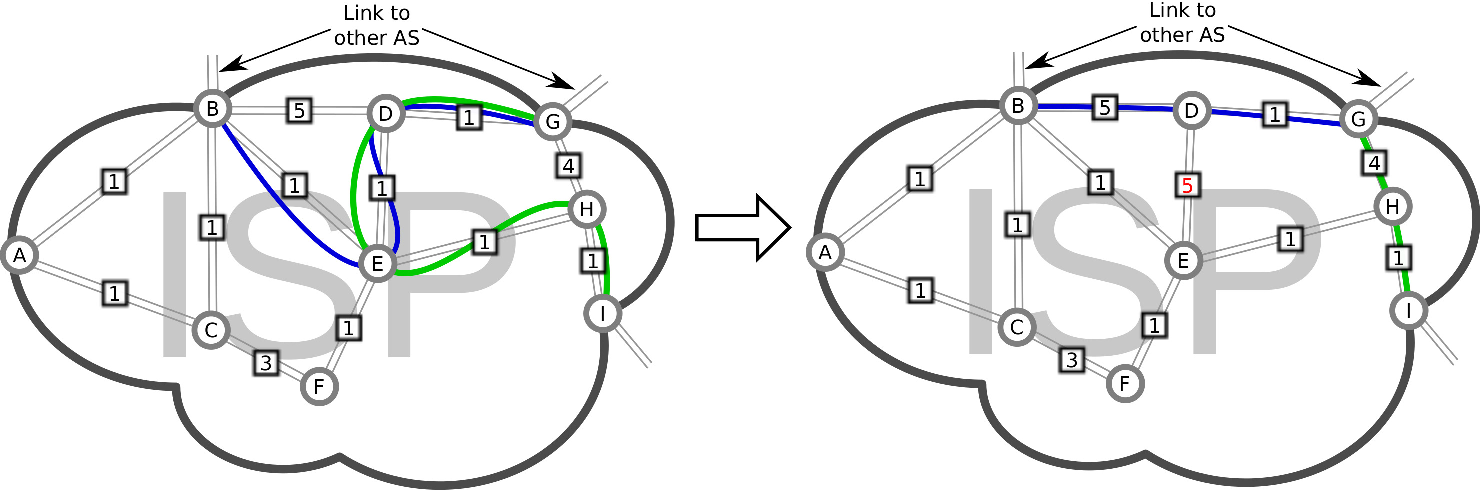
\includegraphics[width=1\linewidth]{figures-pdf/Classic-TE} 
\end{center} 
\caption{IGP based Traffic Management Example} 
\label{fig:SimplifiedTE} 
\end{figure}

The greatest challenge for an ISP is to keep its infrastructure operating
efficiently. This is especially hard, since the ISP itself controls neither the
behavior, nor the source nor destination of the majority of the traffic it
carries. The destination of the traffic is determined by the end-users the ISP
sells services to, while the source is usually operated by a Content Delivery
Infrastructure (CDI). The behavior is dictated through end-users requesting
content, and by the operational choices of the CDI. ISPs today tackle the
problem of network operation efficiency by performing Traffic Engineering (TE).
In its broadest sense, today's TE encompasses the application of technology and
scientific principles to the measurement, characterization, modeling, and
control of Internet traffic~\cite{Awduche_OverviewTE:2002}. Today, traffic
engineering reduces to controlling and optimizing the routing function and to
steering traffic on an Origin-Destination (OD) flow basis through the network
in the most effective way.

Traffic Engineering encompasses multiple steps in order to be performed
successfully. First, an ISP needs to record its traffic volume in terms of
Origin-Destination flows. This means keeping traffic statistics of how much
traffic flows from one router in the network to another. Once the OD flows have
been successfully recorded, TE uses this information to simulate the network
behavior with different IGP configurations. The goal of these simulations is to
find an IGP configuration that spreads the network load as evenly as possible.

Figure~\ref{fig:SimplifiedTE} shows an example of how an IGP configuration can
be used to engineer traffic. The labeled circles represent routers, while the
numbers in the squares represent the IGP-weight for the link. For ease of
presentation, the weights for each link are set to the same value for both
directions. An OD flow, which starts at one router and finishes at another,
takes the path through the network that yields the smallest sum over all
weights along the path. For example, in the starting configuration of the
network (Figure~\ref {fig:SimplifiedTE} (left)) the flow $IG$ does not take the
direct path $I \rightarrow H \rightarrow G$ two, since according to the IGP
weights, a more effective path exists. In fact, the path $I \rightarrow H
\rightarrow E \rightarrow D \rightarrow \ G$ has an accumulated weight of 4
instead of 5 (green path). All traffic at router I destined for router G takes
this path. Similarly, all traffic that originates from B and goes to G follows
the path $B \rightarrow E \rightarrow D \rightarrow G$ (blue path). Also, both
paths share links, leading to a possible overload situation. In order to solve
this problem, we choose to modify the link weight between the routers D and E.
By increasing the weight from 1 to 5 (marked red in the right network), the
blue as well as the green paths are shifted to the direct path. The change is
shown in Figure~\ref{fig:SimplifiedTE} (right).

This simple diagram allows for illustrating multiple caveats that IGP based
traffic engineering introduces. First, IGP-based traffic engineering affects
traffic on an OD-flow basis only. This means that the path from one router to
another can be changed, but the traffic on the OD flow cannot be split onto
multiple paths. Secondly, the change of one weight can affect multiple OD-flows
at the same time. Thus, the weights have to be changed very carefully. In the
worst case, it might not be possible to fully separate some OD-flows due to the
network layout.

One caveat is not immediately obvious but needs to be taken into account when
performing traffic engineering. While the link weights are usually known to all
routers, they are propagated by messages that routers exchange. This
propagation takes time, which can lead to short-term inconsistencies in the
view of a network. We again use Figure~ \ref{fig:SimplifiedTE} for illustrating
this. When the link weight is changed as described in the example explained
before, routers D and E update their routing. This has an immediate effect on
the traffic from B to G. With the update, the shortest path from router E to G
is now $E \rightarrow H \rightarrow G$. In accordance, E configures its routing
to send all traffic for G through H. However, H has not converged at this point
and still uses the old path ($H \rightarrow E \rightarrow D \rightarrow G$).
Thus, H still sends all traffic for G towards E. As long as H uses the outdated
IGP weight information, all traffic for G that reaches either E or H is sent
back and forth between the two routers. This forwarding, on the one hand,
likely overloads the link. On the other hand, most traffic that is affected by
this will be dropped due to its time-to-live (TTL) running out.

The work of Francois \etal~\cite{transient-IGP} shows that it is possible to
gradually change IGP weights by sequentially ordering changes. Accordingly,
routing loops like those in the example are avoided. However, these changes
still require time during which the network can be in a transient state with
overloaded links. Besides the challenges induced by optimizing the IGP, this
approach also assumes that traffic is predictable and stable over time. By
running simulations based on past traffic aggregates to engineer the routing
for the future, it is implicitly assumed that traffic patterns remain similar
over a longer period of time.

With the emergence of CDIs, however, traffic has become volatile in terms of
its origin. In fact, CDIs can shift massive amounts of traffic in a matter of
seconds from one server cluster to another. While this behavior is needed and
propagated by CDIs to cope with volatile demand surges, it is in stark contrast
to the ISP's traffic engineering, which assumes traffic behavior to be stable
for days, weeks or sometimes months.


%%%%%%%%%%%%%%%%%%%%%%%
\subsection{Domain Name System Basics}\label{sec:DNS}
%%%%%%%%%%%%%%%%%%%%%%%

\begin{figure}[tbp] \begin{center}
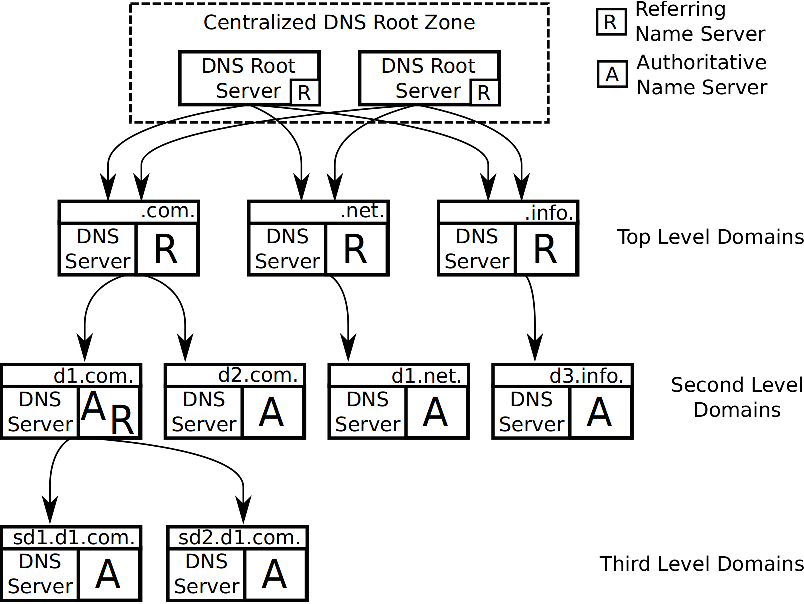
\includegraphics[width=0.8\linewidth]{figures-pdf/DNSHierarchy} 
\end{center}
\caption{Example DNS hierarchy} 
\label{fig:DNS-Hierarchy} 
\end{figure}

The Domain Name System (DNS) plays a major role in today's Internet
architecture and is an essential component of any Web based content delivery
architecture.  DNS relies on a distributed database with a hierarchical
structure. The root zone of the DNS system is centrally administered and serves
its {\em zone} information via a collection of {\em root servers}.  The root
servers delegate responsibility for specific parts (zones) of the hierarchy to
other {\em name servers}, which may in turn delegate the responsibility to
other name servers.  At the end, each site is responsible for its own {\em
domain} and maintains its own database containing its information and operates
an {\em authoritative} name server.

The whole DNS database is usually queried by end-hosts using a local name
server called {\em caching resolver}. If this name server receives a query for
a domain that it does not know about, it fetches this information from another
name server. If the server does not know how to contact the authoritative
server for a zone, it will query a root server\footnote{The first query can go
to some authoritative server below the root if there exists cached
information.}. The root server will \emph{refer} the resolver to another server
that is authoritative for the domain that is immediately below the root and of
which the zone is a part. The resolver will then query this server, and so
forth, stepping down the tree from the root to the desired zone.

To illustrate this process, Figure~\ref{fig:DNS-Hierarchy} show a sample DNS
hierarchy. In this case, the root of the DNS name space, denoted with a '.', is
hosted on two \emph{DNS root servers}. Both servers are under one
administrative control, and both can refer a request to any of the top level
domain servers. Here, three domains exist, \ie \textit{.com}, \textit {.net}
and \textit{.info}. Again, these name servers refer to the second level
domains. Since the domain name are concatenated together as the hierarchy is
traversed, the domains that are now possible are \textit {d1.com.}, \textit
{d2.com.}, \textit{d1.net.} and \textit{d3.info.}. At this point, the second
level domains d1.net. and d3.info have reached their authoritative resolver.
For example, a query to the name server of \textit{.d3} for
\textit{www.d3.info} is answered authoritatively from there. Note that the name
servers for the second level domains are operated by independent entities that
know nothing of each other. Thus, the database is distributed, while each party
is responsible for its own zone.  Finally, the name server of \textit{.d1.com.}
has a dual role. While it is referring the subdomains \textit{.sd1.d1.com.} and
\textit{.sd2.d1.com.} to other name servers, it also answers queries for other
names in its name space authoritatively.  This means that a query for
\textit{www.d1.com.} is directly answered, while a query for
\textit{www.sd1.d1.com} is referred to the name server responsible for
\textit{.sd1.d1.com}.

For efficiency reasons DNS relies heavily on caching
\cite{DNS-caching,DNS-IMC-2010}. All information that a name server delivers to
a resolver is cached for a duration specified in the time-to-live (TTL) field
of the {\em resource records} (RR). Caching today is usually also performed on
end-hosts by the operating system's {\em stub resolver}, as well as
applications, \eg web browsers.

\noindent\textbf{DNS Today.}\label{section:dns-today} When DNS was introduced in
1983, its sole purpose was to resolve host names into IP addresses in a more
scalable fashion than the until then used \texttt{hosts} file. Since then a
number of features and new uses have found their way into the now omnipresent
DNS. In addition to the increasing complexity within the DNS protocol itself
\cite {DNSComplexity2007}, new and oftentimes unforeseen (ab)uses have been
established. Paul Vixie gives an overview in \cite{WhatDNSIsNOT2009}. The most
important points of critique are as follows:

\begin{description} \item[CDI load balancing:] Content delivery infrastructures
set short TTLs on their DNS answers to allow for short reaction times to
shifting loads. Short TTLs impede on cacheability and therefore increase the
load on the whole DNS system. In addition, CDIs tailor their reply for the IP
address of the requesting resolver using the assumption that the DNS resolver
is close to the client originating the request. It has been shown in the past
that this assumption is quite often wrong~\cite
{Precise:Mao2002,dns-redirection,DNS-IMC-2010,DNS-extension-IP-client}.

\item[NXDOMAIN catcher:] Some ISPs and third party DNS providers mangle a
negative reply with the NXDOMAIN status code into a positive one with the IP
address of a search website under the control of the ISP. By hosting
advertisements along the search results it is easily possible to increase the
profit margin. While this may work to some degree for web browsing,
applications relying on proper delivery of NXDOMAIN records, \eg email, are
inevitably hampered.  \end{description}

A third-party ecosystem around DNS has evolved over the last couple of years.
Players like OpenDNS, AdvantageDNS, UltraDNS, and most recently Google offer
open resolvers to anyone with different feature sets. OpenDNS Basic does
NXDOMAIN catching but offers phishing and botnet protection for free.
Furthermore, OpenDNS increases the service level for payment between 5 dollars
a month up to several thousand dollars per year for business customers. When
Google Public DNS entered the market, their highest-valued goals were to
``speed up your browsing experience'' and to ``improve your security''. To
achieve both targets Google advertises an impressive list of optimizations and
fine tuning~\cite{googledns}, \eg prefetching, load balancing with shared
cache, validity checking, and nonce prepending. Google Public DNS also refrains
from utilizing NXDOMAIN to make profit. From an implementation perspective,
most if not all of the third-party resolvers host their DNS servers on multiple
sites around the globe and use anycast to guide DNS clients to the nearest
resolver.

In this open market space a user annoyed by his ISP's DNS can easily choose for
cost-free third-party service.  Tools such as namebench~\cite{namebench} might
help him in choosing a well-performing one. The irony however is that a user,
by choosing a different DNS than the one assigned by his ISP, will most likely
undermine the traffic matrix optimizations performed by CDIs and ISPs, and can
potentially even lower his quality of experience due to longer download
times~\cite{DNS-IMC-2010}.

%
%\newpage
%%%%%%%%%%%%%%%%%%%%%%%%%%%%%%%
\section{Traffic Trends: Overall}\label{sec:traffic}
%%%%%%%%%%%%%%%%%%%%%%%%%%%%%%%

Before delving into the details of the collaborating opportunities for content
providers and infrastructures we embark on giving an overview of typical
characteristics of Internet traffic.  We start by summarizing previous studies
on how Internet traffic looks like. We consider four aspects: \first The
composition of the application mix, \second popular content-types, \third the
distribution of traffic over the course of a day, and \fourth the distribution
of connection sizes.

\subsection{Application Mix}\label{sec:related:appmix}


One constant in the Internet during the last 10 years has been its steady
growth by more than 50\perc each year~\cite{andrew03growth,telegeography2008}.
Initially, protocols such as FTP, SMTP, and NNTP were popular. Then, in about
1994, HTTP entered into the picture. Until 2000, P2P protocols such as Napster
and Gnutella became popular but were later overtaken by eDonkey and BitTorrent.
However, the traffic mix has undergone substantial changes. Therefore, we now
revisit previously reported results regarding the application mix of Internet
traffic. For this purpose we rely on various studies that report on the
application mix between 2007 and 2009 from different vantage points:

\begin{itemize*}

\item The study by Maier \etal~\cite{OnDominantCharacteristics2009}, which is
based on a subset of the traces studied in Section~\ref{sec:impact}. It was
presented at IMC\,'09.

\item Two studies by ipoque~\cite{ipoque09}, which report on different regions
in the world (Germany and Middle East).  These studies are available for
download after registration via a Web form.

\item The Arbor report~\cite{arbor} on the ATLAS Internet Observatory presented
at a recent NANOG\footnote{NANOG is the North American Network Operators
Group.} meeting.

\item The Sandvine report on ``Global Broadband Phenomena''~\cite{sandvine}.

\end{itemize*}

In order to compare the results we have to summarize and unify the traffic
categories as each study uses their own nomenclature (see
Figure~\ref{fig:related:appmix}). For this purpose we use the following seven
categories:

\begin{description}

\item [Web.] All HTTP traffic including One-Click-Hosters (OCHs or Direct
Download Providers) but excluding video and audio streaming over HTTP (\ie
Flash-Video).

\item [Streaming.] All types of streaming in the Internet including streaming
over HTTP, RTP, RTSP, RTMP, ShoutCast, etc.

\item [Usenet.] The article reading and posting system that evolved from UUnet
and which uses NNTP as protocol.

\item [BitTorrent/P2P.] The popular P2P-protocol BitTorrent and all other P2P
traffic that is not eDonkey. Note, that the P2P traffic that is not BitTorrent
or eDonkey only adds a tiny fraction.  Moreover, this category represents all
P2P traffic if the study no further subdivides P2P traffic. This is the case
for Arbor~\cite{arbor} and Sandvine~\cite{sandvine}. Note as well, that the
Arbor study~\cite{arbor} reports a table with traffic shares, stating 0.95\perc
for P2P. This table is annotated with the comment that P2P is more likely to
account for 18\perc based on payload inspection of a limited data subset.

\item [eDonkey.] Another P2P protocol, if reported.

\item [Other/known.] Other identified traffic, for details we refer to the
corresponding studies.

\item [Unclassified.] Traffic that has not been classified. Note, that the
Sandvine~\cite{sandvine} study does not mention unclassified traffic, which
either implies a minute fraction or that it is missing in the plot.

\end{description}

\begin{figure}[tbp]
\centering
\includegraphics[width=0.95\linewidth]{figures/appmix.eps}
\renewcommand{\capname}{Barplot of the application mix in the
Internet\xspace}
\caption[\capname]{\capname (unified categories) for different years,
different regions according to several
sources~\cite{OnDominantCharacteristics2009,ipoque09,arbor,sandvine}.
\capcomment (BitTorrent/P2P contains all P2P except eDonkey.)}
\label{fig:related:appmix}
\end{figure}

Looking at these statistics we find that all studies report a significant
fraction of Web traffic. Indeed, Web is dominant ($>$ 50\perc) in most studies,
followed by P2P and streaming. It is noteworthy that Usenet is responsible for
a non-negligible fraction in several studies. This is surprising and a good
example for the importance of revisiting the application mix periodically in
order to identify new trends.

In terms of P2P protocol distribution Figure~\ref{fig:related:appmix} shows
that BitTorrent is dominating and the shares of eDonkey are decreasing.  Thus,
we note that the results of Plissonneau \etal~\cite{plissonneau05} who observed
91\perc of the P2P traffic is due to eDonkey in 2004 are no longer applicable.
Indeed, the popularity among P2P protocols swapped in favor of BitTorrent. We
can also see a general trend: P2P is declining according to all studies. This
is also supported by the results of Anderson~\cite{p2pdrops}. He points out
that this decline comes with an increase in video streaming. Moreover, most of
the studies pointed out that currently One-Click-Hoster (\eg Rapidshare or
MegaUpload) are as important for file-sharing as P2P systems.

Of course there are also trends that do not impact the application mix, for
example Online Social Networks (OSNs) such as Facebook. This is due to the fact
that OSNs use HTTP and they do not transport large videos, but profile
elements. Nevertheless, OSNs are not unimportant given the huge number of OSN
users world-wide.


\subsection{Content-types in the Internet}\label{sec:related:ctypes}

Next, we turn to the popularity of content-types in the Internet. Again, we
leverage several data sources, namely Maier
\etal~\cite{OnDominantCharacteristics2009}, ipoque~\cite{ipoque09}, and Erman
\etal~\cite{network-caching}. Once more we unify the categories and present
results for contents transferred via BitTorrent, eDonkey, and HTTP. See
Figure~\ref{fig:related:ctypes} for a summary.

\begin{figure}[tbp]
\centering
\includegraphics[width=0.95\linewidth]{figures/ctypes.eps}
\renewcommand{\capname}{Barplot of content-type popularity in the
Internet\xspace}
\caption[\capname]{\capname (unified categories) for
different protocols, different regions according to several
sources~\cite{OnDominantCharacteristics2009,ipoque09,network-caching}.}
\label{fig:related:ctypes}
\end{figure}

We see that videos are the most popular content in P2P systems (BitTorrent and
eDonkey). Even in HTTP videos account for more traffic than any other category.
Although HTTP was designed to transfer Web pages (text, \eg HTML, XML, CSS,
JavaScript, and image files) these contribute less than a third of the total
HTTP volume.

Overall, a significant fraction of software and archives is noticeable.
According to Maier \etal~\cite{OnDominantCharacteristics2009} almost all videos
are in flash-video format and are served by video portals such as YouTube.
Similarly, almost all archives are served by One-Click-Hosters. This is
confirmed by the results of Erman \etal~\cite{network-caching}.

Shifts in the popularity of content-types can be another indicator of new
trends. For example, there have been almost no flash-videos before the
breakthrough of YouTube.



\subsection{Time-of-day Effects}\label{sec:related:tod}

In order to understand when people are active in the Internet we show
time-of-day usage plots of link utilization from Maier
\etal~\cite{OnDominantCharacteristics2009} in
Figure~\ref{fig:related:tod-maier}, and aggregated traffic volume
Sandvine~\cite{sandvine} in Figure~\ref{fig:related:tod-sandvine}.

\begin{figure}[tbp]
\centering
\includegraphics[angle=-90,width=0.85\linewidth]{figures/maier-tod.eps}
\renewcommand{\capname}{Timeseries of link utilization from Maier \etal}
\caption[\capname]{\capname~\cite{OnDominantCharacteristics2009}}
\label{fig:related:tod-maier}
\end{figure}


\begin{figure}[tbp]
\centering
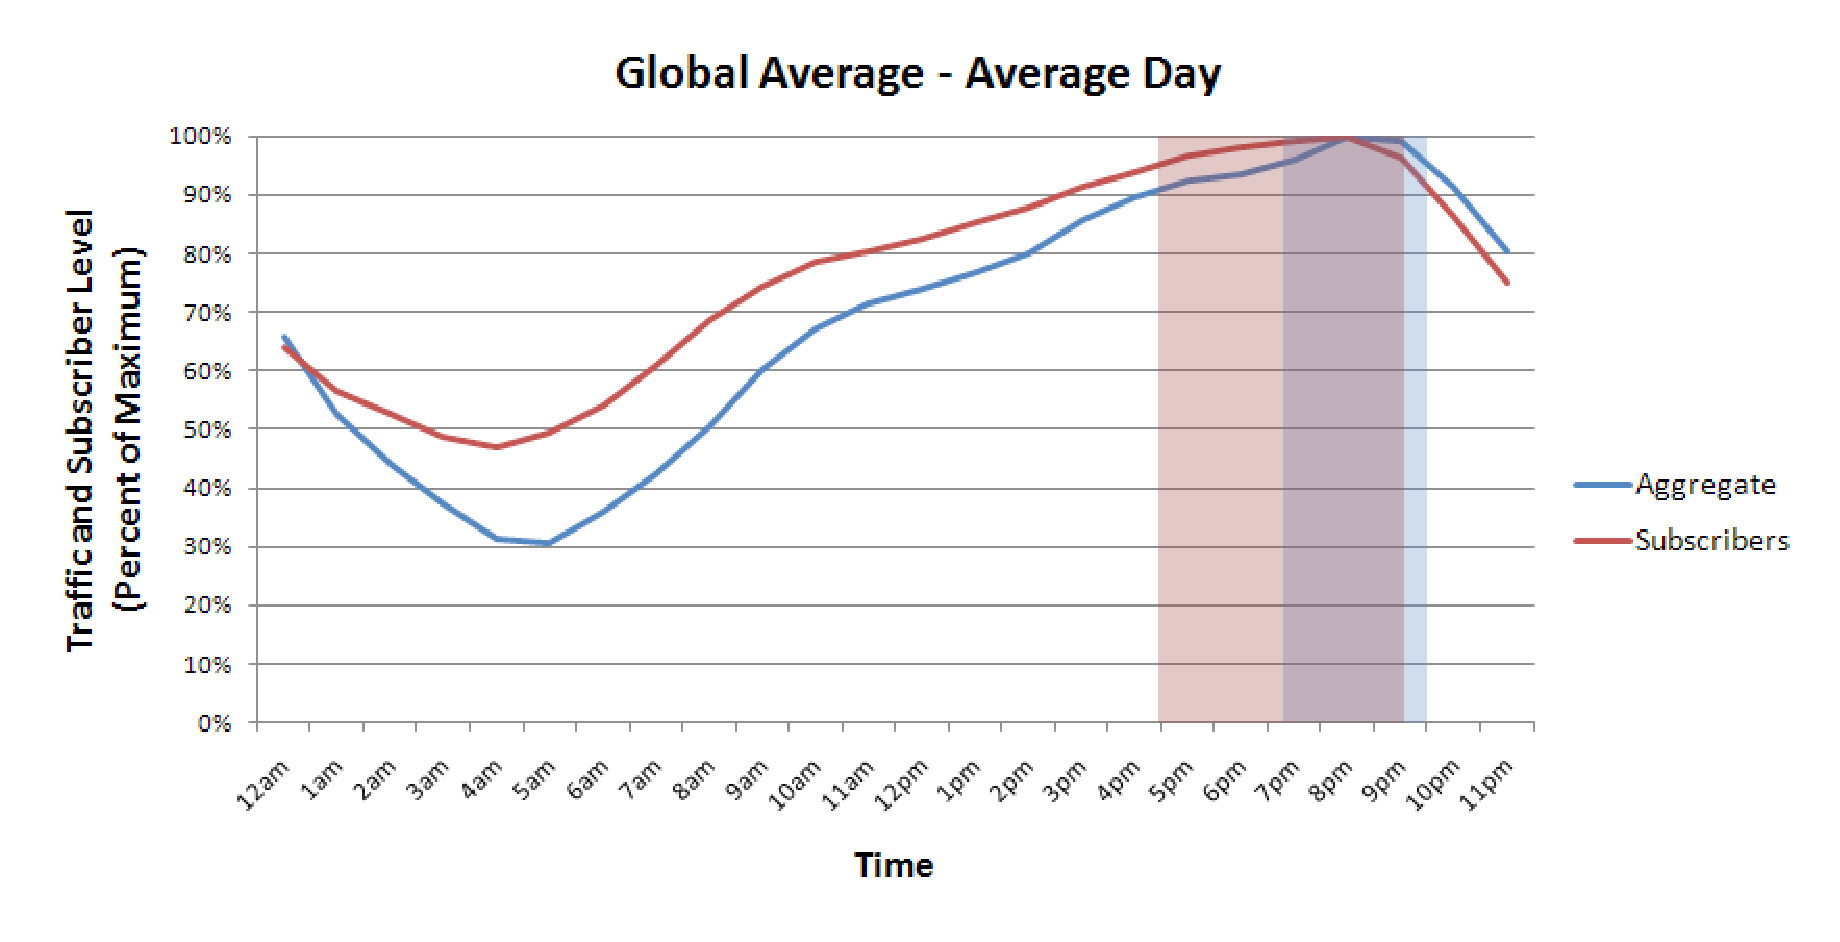
\includegraphics[width=0.85\linewidth]{figures/sandvine-tod.eps}
\renewcommand{\capname}{Timeseries of traffic volume from Sandvine\xspace}
\caption[\capname]{\capname~\cite{sandvine}}
\label{fig:related:tod-sandvine}
\end{figure}

In general, we observe a peak utilization at prime-time around 8\,pm and a
daily low between 2\,am and 4\,am. As the data sets of all these studies are
primarily collected from residential networks, it not surprising that they all
show similar characteristics. The peak usage in the evening hours can easily be
explained by the fact that people are usually not at home during business
hours. Rising demands just before lunch and in the afternoon may be due to
children returning home from school.


%
%\newpage

%%%%%%%%%%%%%%%%%%%%%%%%%%%%%%%
\section{Traffic Trends: Content Server Diversity}\label{sec:traffic-diversity}
%%%%%%%%%%%%%%%%%%%%%%%%%%%%%%%

So far we have highlighted that the Web and P2P protocols are responsible for a
major share of the Internet traffic. However, we have not yet explored if all
content is equally popular or if a few content providers dominate. This is the
goal of this section.

Our evaluation methodology relies on packet level traces from a large European
ISP. We analyze them towards identifying CDI infrastructures and their behavior
as seen by an ISP. Here, we find that CDIs rely on the domain Name System (DNS)
for their operation. Thus, we focus our analysis on the DNS infrastructure in
order to find the server deployment, mapping and operational behavior of CDIs.
Based on these observations, we develop classification methods to detect CDI
infrastructures and perform a first potential analysis on the impact of CDI
operation when basic ISP knowledge is available.

\subsection{Residential ISP Traces}\label{sec:traces} We base our study on
three sets of anonymized packet-level observations of residential DSL
connections collected at aggregation points within a large European ISP.  Our
monitor, using Endace monitoring cards, allows us to observe the traffic of
more than 20,000~DSL lines to the Internet.  The data anonymization,
classification, as well as application protocol specific header extraction and
anonymization is performed immediately on the secured measurement
infrastructure using the Bro NIDS~\cite{bro-paper} with dynamic protocol
detection (DPD)~\cite {dreger06dpd}.

We use an anonymized 24\,h packet trace collected in March 2010 (\martrace) for
detailed analysis of the protocol behavior. For studying longer term trends, we
used Bro's online analysis capabilities to collect an anonymized protocol
specific trace summary (\httplong) spanning 2 weeks. Additionally, we collected
an anonymized 5\,day DNS trace (\dnslong) in February 2010 to achieve a better
understanding of how hostnames are resolved by different sites. Due to the
amount of traffic at our vantage point and the resource intensive analysis, we
gathered the online trace summaries one at a time. Table \ref{tab:traces}
summarizes the characteristics of the traces, including their start, duration,
size, and protocol volume.  It is not possible to determine the exact
application mix for the protocol specific traces, as we only focus on the
specific protocol.  However, we use full traces to cross check the general
application mix evolution.

\begin{table*}
  \small
    \begin{center}
      \tabcolsep2mm
      \begin{tabular}{l|l|l@{ }l|r|r|r}

      Name      & Type     & \multicolumn{2}{|l|}{Start date} & Dur. & Size        & Application Volume \\
      \hline
      \martrace & packet   & 04 Mar'10    & 2am    & 24~h      & $>$5\,TB    & $>$ 3\,TB HTTP, $>$ 5\, GB DNS \\
      \hline
      \httplong & log file & 09 Sep'09    & 3am    & 14~d      & $>$ 200\,GB & corresponds to $>$ 40\,TB HTTP \\
      \dnslong  & packet   & 24 Feb'10    & 4pm    & 5~d       & $>$25\,GB   &  $>$ 25\,GB DNS \\
      \end{tabular}
    \end{center}
    \vspace*{-1\baselineskip}
    \caption{Summaries of anonymized traces from a European ISP}%
    \label{tab:traces}
\end{table*}

With regards to the application mix, recall Section~\ref{sec:traffic}, Maier et
al.~ \cite{OnDominantCharacteristics2009} find that HTTP, BitTorrent, and
eDonkey each contribute a significant amount of traffic, see Table
\ref{tab:traces}.  In \martrace HTTP alone contributes almost 60\perc of the
overall traffic at our vantage point, BitTorrent and eDonkey contribute more
than 10\perc. Recall that similar protocol distributions have been observed at
different times and at other locations of the same ISP, see
Figure~\ref{fig:related:appmix} summarizes the results. Note that almost all
streaming is done via the Web on top of HTTP.  Therefore, we conclude that
currently HTTP is the dominant service and P2P is still responsible for at
least 15\% of the traffic.

Analyzing \httplong, we find more than 1.2 billion HTTP requests, or 89 million
requests per day on average. This is consistent with 95 million requests in 24
hours in \martrace. The advantage of using click stream data from a large set
of residential users is their completeness. We are, e.g., not biased by the
content offered \first by a web service, \second whether sufficient users
installed measurement tools such as the \url{alexa.com} toolbar, or \third
whether users actually use some kind of Web proxy.

To identify the most popular web services, we focus on the most popular hosts.
As expected, the distribution of host popularity by volume as well as by number
of requests is highly skewed and is consistent with a Zipf-like distribution as
observed in other studies~\cite{OnDominantCharacteristics2009}. The top 10,000
hosts by volume and the top 10,000 hosts by number of requests together result
in roughly 17,500 hosts.  This indicates that on the one hand, some hosts that
are popular by volume may not be popular by number of requests and vice versa.
On the other hand, there are some hosts that are popular according to both
metrics.  The total activity by these hosts accounts for 88.5\perc of the
overall HTTP volume and more than 84\perc of the HTTP requests. Assuming that
the HTTP traffic volume accounts for roughly 60\perc of the total traffic,
similar to the observations made in September 2009~\cite{OnDominantCharacteristics2009,UGCcacheability} 
and in \martrace, more than 50\perc of the trace's total traffic is captured by
these hosts.

\begin{figure}[tbp]
  \centering
  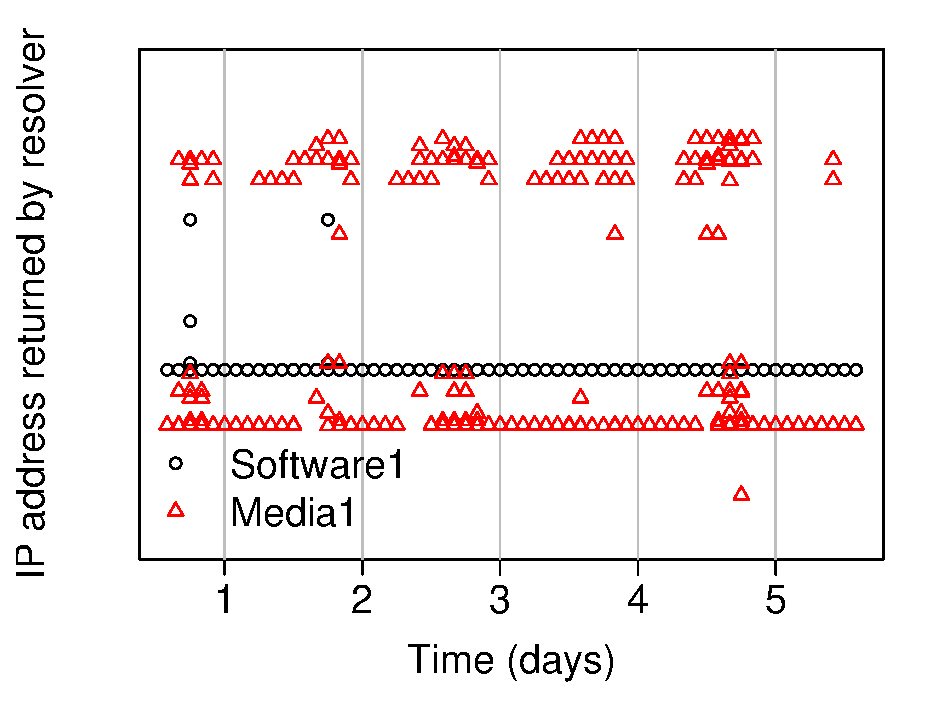
\includegraphics[height=0.7\linewidth]{figures/dns-diversity.eps}
  \caption{DNS replies for two different sites hosted on a CDI, in two-hour bins}%
  \label{fig:dns_diversity}
\end{figure}


\subsection{Server Diversity and DNS Load Balancing}\label{sec:active_dns_measurement} 

To better understand how HTTP requests are handled and assigned to servers, we
use \dnslong to analyze the 20 most heavily queried DNS names to identify
typical usage patterns. We consider only the most heavily used resolver.
Figure~\ref{fig:dns_diversity} shows two of the typical patterns for two of the
DNS names. It also shows how the resolved IP addresses change (y-axis) across
time (x-axis) for two hostnames; respectively a software site, labeled
Software1, and a media site, labeled Media1. The vertical lines annotate
midnight. If two IP addresses are plotted close to each other, this indicates
that the longest common prefix of the two addresses is close. We note that the
hostname of Software1 is mainly resolved to a single subnet, excepting a few
special cases. However, Media1 is load balanced across approximately 16
different sites. For Media1, there appears to be one main site which is almost
always available, while the remaining 15 are predominantly used during
afternoon and evening peak usage hours.

These results are promising, and show that individual sites do expose a certain
degree of server diversity to their users. While our trace (\httplong) includes
the queried hostnames, it does not include the resolved IP address, as a HTTP
request header contains the hostname but not the IP address of a server. To
verify the above behavior and get an up-to-date view of the DNS replies for the
hostnames of our trace, we used 3 hosts within the ISP to issue DNS queries to
the ISP's DNS resolver for all 17,500 hostnames repeatedly over a fourteen day
measurement period starting on Tue Apr 13th 2010. During these two weeks, we
received more than 16 million replies. Unless otherwise mentioned, we rely on
our active DNS measurements, with augmented statistics concerning volume and
requests from \httplong.

\subsection{Server Location Diversity}\label{sec:server_location_diversity}


Our analysis of hostnames and their assignment to servers in section
\ref{sec:active_dns_measurement} has shown that content can be served by
multiple servers in different locations. In fact, many domains use the service
of a \textit{Content~Delivery~Infrastructure} (CDI), which can be seen during
the DNS resolution progress: The original domain name is mapped to the domain
of a CDI, which then answers requests on behalf of the requested domain name
from one of its caches~\cite{DraftingAkamai:SIGCOMM2006}. Almost all CDIs rely
on a distributed infrastructure to handle the expected load, load spikes, flash
crowds, and special events. Additionally, this introduces needed redundancy and
fail over configurations in their services. Among the most studied CDI' are
Content Distribution Networks (CDNs), such as Akamai~\cite
{ImprovingPerformanceInternet2009, DraftingAkamai:SIGCOMM2006,
MeasuringAndEvaluating2008}, and Content Delivery Platforms (CDPs), such as
Google~\cite{MovingBeyondE2E2009} and their YouTube service~\cite {YouTube}.

\begin{figure}[tbp]
   \center
   \includegraphics[height=0.7\linewidth,angle=-90]{figures/avgResponseSize.ps}\\
   \includegraphics[height=0.7\linewidth,angle=-90]{figures/avgResponseSubnetSize.ps}

  \caption{CCDF of mean \# of IPs (top) and subnets (bottom) per DNS reply for the ISPs DNS resolver.}
  \label{fig:CDF-AVG-REPLY-IPs}
\end{figure}

The DNS server can choose to return one or more server IP addresses based on
the domain name in the request and the IP address of the requesting DNS
resolver. For example, it may use a geo-location database~\cite{MaxMind} to
localize the region of the DNS resolver, utilize BGP data to identify the ISP,
create a topology map derived via traceroutes, or any combination of these and
other topological and geographic localization techniques. A DNS server has, in
principle, two methods for load balancing across multiple servers:

\begin{description*}
\item[MultQuery:] Can return multiple IP addresses within a single DNS response
\item[CrossQuery:] Can return different IP addresses for repeated queries and
  thus perform DNS redirection.
\end{description*}

In our active DNS measurements, we found that often a mixture of MultQuery and
CrossQuery is being used in practice. Furthermore, we used the measurement
results to \first map hostnames to sets of IP addresses and \second check the
IP address diversity of these sets for a better understanding of server
diversity and their location. We achieved this by aggregating the returned IP
addresses into subnets based on BGP information obtained from within the
ISP. This allows for detailed information about the different locations within
the ISP, while giving an aggregated view of subnets reachable via peering
links.

Another issue stems from the fact that the IP address returned by the CDI
depends on the IP address of the ISP DNS
resolver~\cite{DNS-IMC-2010,dns-redirection,DraftingAkamai:SIGCOMM2006}. Due to
this, we used the DNS resolver of the ISP of our vantage point as well as
external DNS resolvers (see section \ref{sec:dns_resolvers}). The former
reflects the experience of most of the clients at our vantage point\footnote{We
verify using the traces that more than 95\perc of the clients use the ISP's DNS
resolver as their default one. }. The latter lets us discover additional
diversity as well as understand the preference of the CDI for this specific
ISP.

\begin{figure}[tbp]
  \center
   \includegraphics[height=0.7\linewidth,angle=-90]{figures/14day-returnedIPCDF-bytes.ps}
   \includegraphics[height=0.7\linewidth,angle=-90]{figures/14day-returnedIPCDF-hits.ps}
  \caption{CDF of \# of IPs for the ISP DNS resolver normalized by traffic
    volume  (top) and requests (bottom) including aggregation on
    domain levels. (Logarithmic x-axis.)}
  \label{fig:CDF-IPPAF-IPs}
\end{figure}

\begin{figure}[tbp]
  \center
   \includegraphics[height=0.7\linewidth,angle=-90]{figures/SubnetsByBytes.ps}
   \includegraphics[height=0.7\linewidth,angle=-90]{figures/SubnetsByHits.ps}
  \caption{CDF of \# of subnets for ISP DNS resolver normalized by traffic
    volume  (top) and by requests (bottom) including aggregation on
    domain levels. (Logarithmic x-axis.)}
  \label{fig:CDF-IPPAF-Subnets}
\end{figure}

\paragraph{Prevalence of MultQuery.} We start our analysis by checking the
prevalence of the first form of DNS based load balancing, MultQuery. Figure~
\ref{fig:CDF-AVG-REPLY-IPs} shows a CCDF plot of the average number of IP
addresses (top) and subnets (bottom) per DNS reply. In addition, we included
the same data normalized by traffic volume and number of requests.

A first observation is that the number of returned IP addresses per request is
rather small. The median is $1$, the average is $1.3$ and even the $0.9$
percentile is $2$. We note that even when an answer yields multiple IP
addresses, the majority of them are from the same subnet. Therefore, the
diversity decreases even further if we aggregate to subnets. From a network
perspective, this implies that there is not much choice, neither for the ISP
nor for the user, regarding where to download the content from. Both are
limited to the information provided by the DNS server. However, when we
normalize the hosts by their respective popularity, we see a significant
improvement. More than $29$\% of the volume and $19$\% of requests have a
choice among at least $2$ IP addresses.

\paragraph{Prevalence of CrossQuery.} Next, we check how prevalent CrossQuery,
the second form of DNS based load balancing is. Since CrossQuery returns
different IP addresses for repeated queries, its potential contribution to
server diversity can only be studied by aggregating across time. The lines
labeled \texttt{Full Domain Name} in Figures~\ref{fig:CDF-IPPAF-IPs} and~\ref
{fig:CDF-IPPAF-Subnets} capture this case.

We find that more than $50$\perc of the volume or requests can be served by
more than one IP address. Similarly, there is choice between at least two
subnets over $40$\perc of the time across both metrics, see Figure~\ref
{fig:CDF-IPPAF-Subnets}. This indicates that there is significant potential for
the ISP to bias the location preference of the CDI.

\begin{figure}[tbp]
  \center\includegraphics[height=0.7\linewidth,angle=-90]{figures/maxTTLCDF.ps}
  \caption{CDF of DNS TTL value by traffic volume and by number of requests.}
  \label{fig:CDF-IPPAF-TTL}
\end{figure}


\paragraph{Subdomain Aggregation.} Since some CDIs only use subdomains as hints
about the context of the requested URLs or the requested services, we
accumulate the answers further regarding the 2nd and 3rd part of the domain
names of the hosts, see Figures~\ref {fig:CDF-IPPAF-IPs}
and~\ref{fig:CDF-IPPAF-Subnets} at the respective data series called
\texttt{3rd Level Domain} and \texttt{2nd Level Domain}. For example, we might
accumulate the IP addresses from DNS replies for \url {dl1.example.org} and
\url{dl2.example.org} for the statistics on the 2nd level domain, but not the
third level domain.

This is a feasible approach, since many hosts respond to all requests that
belong to a subset of the subnets returned when accumulating by the
second-level domain of DNS resolver answer, including recursive requests and
redirections.  This behavior was verified with active measurements
in~\cite{PADIS2010}. We find that at least two major CDIs, a streaming provider
and a One-Click Hoster, serve requested content from servers that match in
their second level domain.

We note that the accumulation by third-level domain, and especially by second
level domain significantly increases the number of observed subnets per request
both normalized by requests as well as by volume.  The number of returned
subnets further increases when accumulating to the second-level domain of DNS
resolver answer. Studying our traces in more detail, we find that this is due
to the substantial traffic volume and number of requests that are served by
CDIs, some of which are highly distributed within ISPs or located in multihomed
datacenters or peer-exchange points.

\paragraph{Infrastructure Redirection Aggregation.}
Taking a closer look at the DNS replies~\cite{ietf-dns}, we find that some CDIs
use CNAME records to map queried hostname to an A record. These A records show
the same pattern as the hostnames in the previous section: the second level
domain is identical. Similar to the previous approach, we can aggregate by
these A records.


Turning our attention to the implications of the proposed aggregation schemes,
we notice the available diversity increases tremendously. More than 50\% of the
hits and 70\% of the bytes can be served by more than $20$ servers.  With
regards to subnets, the diversity decreases slightly. Nevertheless, more than
$5$ subnets are available for 45 \% of the hits and 55\% of the bytes.

If we consider aggregation periods in the order of tens of minutes, the numbers
do not decrease by much.  The reason that most of the diversity is observable
even over these short aggregation time periods, is that the typical TTL, see
Figure~\ref{fig:CDF-IPPAF-TTL}, is rather short with a mean of $2,100$ seconds
and an median of $300$ seconds normalized by volume. When weighted by requests,
the mean/median is $4,100$/$300$ seconds.

\paragraph{Alternative DNS Resolvers.}\label{sec:dns_resolvers}
So far we have only considered the effect of content diversity when the ISP DNS
resolver is used. To understand how much the DNS load balancing deployed by a
CDI is biased by the queried DNS resolver, we repeat the experiment from
Section~\ref{sec:active_dns_measurement} using two other DNS resolvers. In
particular, we pick the next most popular DNS resolvers found in our traces:
GoogleDNS and OpenDNS. Both are third-party resolvers with a global footprint
and utilize DNS anycast.

Comparing the results, we find that we attain more IP address diversity and
subnet diversity when using the ISP DNS resolver. This is mainly due to the
fact that CDIs select the supplied caches based on the source IP address of the
querying DNS resolver. Since the CDIs are no longer able to map the request to
the AS it originates from, but rather to AS the DNS resolver belongs to, the
server selection by the CDI cannot optimize for the location of the DNS client.

A possible solution to the problem is the EDNS-Client-Subnet
extension~\cite{EDNS}, an extension that utilizes the EDNS0 option field that
is used today by DNS Security Extensions (DNSSEC). A recent study~\cite{EDNS:IMC2012} showed that the
user-to-server allocation can be significantly improved as well as the
end-to-end performance for the client. On the other hand, this requires that
all the involved resolvers and authoritative servers in ISPs, CDNs, third
parties that maintain resolvers and authoritative servers, \eg GoogleDNS, OpenDNS, 
have to support EDNS-Client-Subnet extension.



\subsection{Impact on Traffic Localization}\label{sec:dns_localization}

\begin{table}
  \begin{center}
    \tabcolsep2mm{}
    \begin{tabular}{|c||c|c||c|c||c|c|}
      \hline      & \multicolumn{2}{c||}{ISP DNS} & \multicolumn{2}{c||}{OpenDNS} & \multicolumn{2}{c|}{GoogleDNS}\\
      \hline Metric  & observed  & potential & observed & potential   & observed  & potential   \\ \hline
      \hline IPs     & 12.3\perc & 24.2\perc & 5.8\perc  & 16.0\perc  & 6.0\perc  & 9.7\perc    \\
      \hline requests& 14.9\perc & 33.2\perc & 4.7\perc  & 18.8\perc  & 4.8\perc  & 6.4\perc    \\
      \hline volume  & 23.4\perc & 50.0\perc & 12.0\perc & 27.7\perc  & 12.3\perc & 13.4\perc   \\
      \hline
    \end{tabular}
  \end{center}


  \caption{Traffic localization within the network by different DNS resolvers normalized by number of requests and
  traffic volume together with the potentially available fraction of localized traffic.}
  \label{tab:TraceLocallizedTraffic}
\end{table}

Analyzing the three active DNS measurements from the ISP, OpenDNS as well as
Google DNS resolver, we find that a significant part of the requests that could
have been in principle served by sources within the ISP are directed towards
servers that are outside of the ISP.  However, before tackling this issue, we
need to understand what fraction of the traffic may be served by IP addresses
within the ISP's network and what fraction is served by IP addresses outside of
the AS. To this end, we analyze each of the three active DNS traces
separately. For each trace, we start by classifying all DNS replies regarding
the \texttt{redirection} aggregation described in Section~
\ref{sec:server_location_diversity} and account the volume (or hits) evenly to
each of the IP addresses.  Next, we classify the IP addresses in two groups -
inside and outside of the ISP network.  Table~\ref {tab:TraceLocallizedTraffic}
summarizes the results of this aggregation regarding the traffic and hits that
were kept inside the ISP's network in the columns labeled \texttt{observed}.

Turning to the results, we find that there is hardly any difference between
those clients that use the external DNS resolvers, \ie GoogleDNS or OpenDNS. Of
the returned IP addresses, less than $6$\perc are within the AS. When weighted
by number of requests, this does not change much. However, when normalizing by
volume, about $12$\perc of the traffic stays within the AS. In contrast,
clients that use the ISP's DNS resolver fare better: almost a quarter of the
traffic volume is served from servers within the AS. Normalized by requests, we
see a three fold increase, and normalized by hits or volume, roughly a two fold
increase over using external DNS resolvers.  Among the reasons for the ``bad''
performance of external DNS resolvers is that some CDIs may always return IP
addresses outside the ISP, despite the fact that many of its servers are
deployed within the ISP. The reason behind this is that the CDIs cannot map the
DNS resolver to the AS anymore, and thus are unaware of the origin of the
request. This explains the substantial difference and highlights on the one
hand the effectiveness of the CDI optimization, but also points out its
limits. As such, it is not surprising that there are efforts under way within
the IETF to include the source IP addresses of the DNS client in the DNS
requests~\cite{DNS-extension-IP-client}.

However, one can ask if the CDI utilizes the full potential of traffic
localization on an AS level. For this, we check the potential of traffic
localization, by changing the volume (or hit) distribution from even to greedy.
Thus, as soon as we observe at least one IP address inside the ISP's network,
we count all traffic for the entire aggregation to be
internal. Table~\ref{tab:TraceLocallizedTraffic} shows the results in the
columns labeled \texttt {potential} for all three DNS traces. Note the
substantial differences. Our results indicate that a gain of more than a factor
of two can be achieved. Furthermore, up to 50\perc of the traffic can be
delivered from servers within the ISP rather than only 23.4\perc. This may not
only in itself result in a substantial reduction of costs for the ISP, but it
also points out the potential of collaboration between CDIs and ISPs. While the
increase is noticeable it is nowhere near that of the ISP's DNS resolver. The
potential benefit when relying on GoogleDNS is rather small. A deeper study on
our results unveils that content served by highly distributed and redundant
infrastructures can be localized the most.


\subsection{Summary}\label{sec:diversity_summary}
We find that HTTP is again the dominant traffic source, while the prevalence of
P2P traffic decreases. Since most CDIs rely on distributed infrastructure, we
not only observe significant server location diversity but also significant
path diversity for accessing HTTP based content. Indeed, there is the potential
to bias roughly half of the overall traffic by redirecting queries to different
content servers.

More precisely, we estimate that around $70$\perc of the HTTP traffic in a big
European ISP can be redirected when taking advantage of the diversity due to
MultQuery, CrossQuery and hostname aggregation.  Furthermore, we show that
current CDI optimizations that approximate the location of end-users based on
the location of the local DNS resolvers are more effective than those based on
the location of third-party resolvers. Finally, we show that the traffic
localization potential within the above mentioned ISP is very high especially
when the ISP DNS resolver is utilized.

%
%\clearpage

%%%%%%%%%%%%%%%%%%%%%%%%%%%%%%%%%%%%%%%%%%%%
\section{Content Delivery: An Overview}\label{sec:overview}
%%%%%%%%%%%%%%%%%%%%%%%%%%%%%%%%%%%%%%%%%%%%

While content may be seen as king not all content is equally popular among
users. Indeed, content popularity often follows ``Zipf's law''.  If the
popularity of elements as function of the rank is consistent with a power-law
distribution it is referred to as Zipf's-like (see~\cite{Zipf49,Mitzenmacher03}
and references therein).  The rank is determined by the number of occurrence of
an element, where a low rank index refers to a popular element.  Not
surprisingly Zipf's law does not only apply to the popularity of content but
also quite a number of different quantities in Internet traffic, including the
popularity of Web pages~\cite{breslau:99,SerpanosKarakostasWolf:00}, traffic
demands~\cite {Fang_Peterson:1999, feldmann:00,
ZhangBreslauPaxsonShenker2002,Wallerich:2005, BrownleeClaffy02}, as well as
interdomain Web traffic demands~\cite{Feldmann:Kammenhuber:2004}.  Thus, while
some content can be served by a single server most content, namely the popular
content, can only be served if it is highly replicated across multiple servers.
Thus, one of the main challenges in content delivery is {\bf{server
selection}}. Server selection means identifying a specific server from which
the request for content by a user is satisfied.

Content delivery and the network infrastructure interact mostly through content
source selection, often called server selection. Here, it does not matter
whether the source is a server pushing content through HTTP or from a peer in a
P2P network. In the case of HTTP, the domain name system (DNS) is the preferred
mechanism for performing server selection. In the case of P2P, peer selection
strategies drive where the content is obtained from and how, e.g., when the
content is cut into chunks.

To direct users to appropriate servers, CDIs rely extensively on the Domain
Name System (DNS).  We describe this and other server selection mechanisms in
detail later in this section.  The CDI chooses a server based on several
metrics. Criteria for server selection include the IP address of the end-user's
DNS resolver, the availability of the server, the proximity of the server to
the resolver, and the monetary cost of delivering the content. Note that the
server selection does not know the client IP address or network location, it
only knows the IP address of the DNS resolver the end-user contacted. A recent
study~\cite {DNS-IMC-2010} showed that sometimes the end-user is not close to
the resolver. To improve the mapping of end-users to servers, the client-IP
eDNS extension~\cite {DNS-extension-IP-client} has been recently proposed.

In P2P systems peers can choose among all other peers to download content from
but only if the have the desired content. Thus the problem of getting content
in a P2P system is actually two-fold: first the user needs to find the content
and once it knows of possible peers it can download the content from, it needs
to connect to some of them to get the desired content.  In P2P systems the
content lookup is realized in many different ways. Some P2P network, called
structured P2P, implement a distributed lookup system most often referred to as
distributed hash table (DHT). Other P2P systems, called unstructured P2P, like
Gnutella, flood search request into the network.  Some systems rely on a
partial centralized infrastructure to obtain content information. We discuss
the different approaches in P2P systems in more detail in
section~\ref{sec:P2P}.

Before we can discuss all the various options on how content delivery can be
improved in the current Internet we give a short overview how a typical Content
Distribution Network operates.


\subsection{Content Delivery Networks} \label{sec:content_delivery}

\begin{figure} \begin{center}
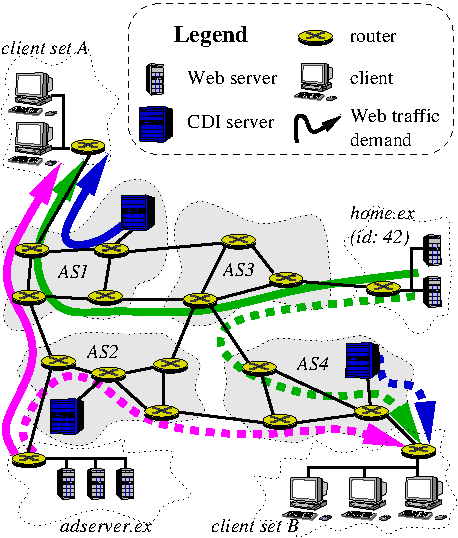
\includegraphics[width=0.7\linewidth]{figures-pdf/flows-example} 
\end{center}
\caption{Example of CDI deployment and traffic flows (Web traffic
  demands). Reprinted from \cite{inferring-web-demand}, \copyright ACM, 2004. Included here by permission.}
\label{fig:aka:cdn} \end{figure}

\begin{figure} 
\begin{center}
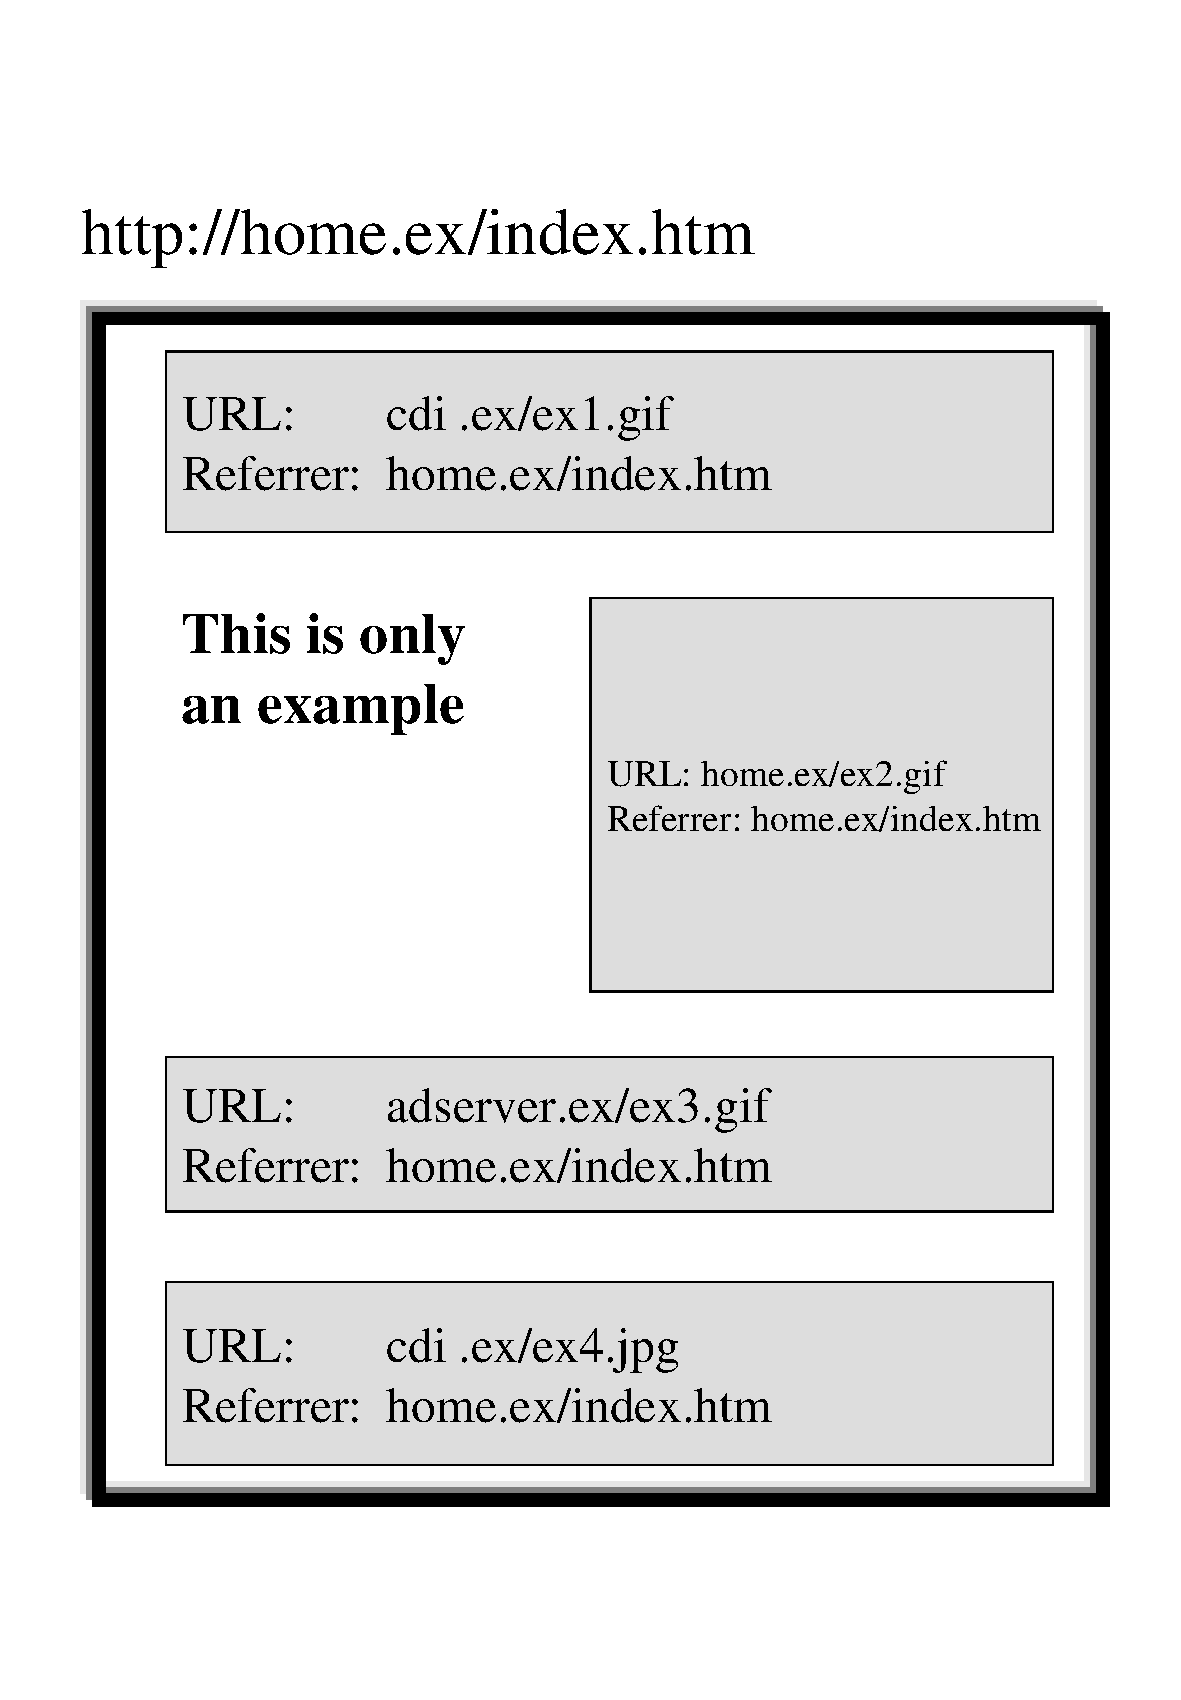
\includegraphics[width=0.6\linewidth]{figures-pdf/page}
\vspace*{-.7cm}
\end{center}
\caption{Example Web page with some CDI content. Reprinted from \cite{inferring-web-demand}, \copyright ACM, 2004. Included here by permission.}
\label{fig:aka:cdn_page}
\end{figure}

Recall content is king in the current Internet and content is typically first
placed on the Web site of the content producer, the original Web servers.
Content Delivery Infrastructures (CDIs) (see,
\eg~\cite{cdn:2002,akamai:2002,gadde01web,bent02whole,johnson00measured,bala:imw01,gribble:osdi02})
are designed to reduce the load on origin servers and at the same time improve
performance for the user.  Most CDIs have a large set of servers deployed
throughout the Internet and cache the content of the original publisher at
these servers.  Therefore another view of CDIs is that they provide reverse
proxy services for content providers, the publishers.  In order to take
advantage of their distributed infrastructure, requests for data are redirected
to the ``closest'' cache server. Intelligent redirection can reduce network
latency and load (and therefore network congestion) improving response time.
CDIs differ in their approach to redirecting traffic. Some (such as
Akamai~\cite{Akamai-Network}), use DNS to translate the hostname of a page
request into the IP address of an appropriate server. This translation may
consider the location of the client, the location of the server, the
connectivity of the client to the server, the load on the server, and other
performance and cost based criteria.

An example that shows how the CDI infrastructure is embedded in the Internet
architecture is shown in Figure~\ref{fig:aka:cdn}. Recall, the Internet is
divided into a collection of autonomous systems (ASes).  Each AS is managed by
an Internet Service Provider (ISP), who operates a backbone network that
provides connectivity to clients and to other ISPs.  Figure~\ref{fig:aka:cdn}
shows four ASes, numbered 1--4, whose backbones consist of three routers each,
two Web site publishers, \url{home.ex} and \url{adserver.ex}, and two sets of
clients. The publisher \url{home.ex} is connected to AS\,3 while the publisher
\url{adserver.ex} is connected to AS\,2. A set of clients is connected to
AS\,1, another to AS\,4.

The location of the CDI's servers differ from CDI to CDI and depends on
contractual agreements between the CDI and the individual ISPs.  In some
instances, the CDI servers are deployed within the data centers of the ISP and
therefore belong to the same AS, like AS\,1,\,2,\,4 in
Figure~\ref{fig:aka:cdn}.  Clients of the ISP (end-users) are typically served
by these servers in the same AS.  With other ISPs, the CDI may have a private
peering agreement that allows the CDI to serve requests from the ISPs clients
via a direct connection between the CDI and the AS.  The CDI may also co-locate
servers with the ISP's clients, \eg on university campuses.  With other ISPs
there may be no relationship with the CDI, and the traffic to the ISP's clients
is routed via another AS.

Let us consider the steps that are necessary to download the Web page shown in
Figure~\ref{fig:aka:cdn_page}. This page consists of one main page located at
\url{home.ex/index.htm} and four embedded objects. The publisher responsible
for \url{home.ex} has decided to use the services of a CDI, \url{cdi.ex}. One
object (\url{ex2.gif}) of the sample page is located on the same server as the
page itself (\url{index.htm}); another object (\url{ex3.gif}) is served by a
company providing dynamic advertisements, \url{adserver.ex}; and objects
\url{ex1.gif} and \url{ex4.jpg} are hosted by the CDI.

If a specific client from client set~A in Figure~\ref{fig:aka:cdn} accesses the
Web page, publisher \url{home.ex}  serves the bytes for the main page and one
embedded object, publisher \url{adserver.ex} serves the bytes for the object
located on its servers, and the ``nearest'' CDI server serves the two
CDI-located objects---in this case, they will be served from AS\,1.  In
contrast, if a specific client from client set~B accesses the page, the two CDI
objects are delivered from a different CDI server, namely the one in AS\,4.
Keep in mind that it is the objective of the CDI to direct the client to a CDI
server that is close to the client.

To complete the picture one question remains. How does the CDI choose the
``nearest'' server to deliver the content from? Today's CDI landscape relies
mainly on three techniques to assign end-users to servers.

\begin{enumerate*}

  \item IP-Anycast

  \item DNS based redirection

  \item HTTP redirection

\end{enumerate*}

While all techniques help the CDIs to assign end-users to their servers, all of
them have different drawbacks. In the following we will explain how the
different techniques work and what those drawbacks are:

\vspace{1em} \noindent \textbf{IP-Anycast.} IP Anycast is a routing technique
used to send IP packets to the topologically closest member of a group of
potential CDI servers. IP Anycast is usually realized by announcing the
destination address from multiple locations in a network or on the Internet.
Since the same IP address is available at multiple locations, the routing
process selects the shortest route for the destination according to its
configuration. Simply speaking, each router in a network selects one of the
locations the Anycasted IP is announced from based on the used routing metrics
(\eg path length or routing weights) and configures a route towards it. Note
that, if a network learns of an Anycasted IP address from different sources, it
does not necessarily direct all its traffic to one of its locations. Its
routing can decide to send packets from region A in the network to location A'
while region B gets a route to location B'. This means that the entire server
selection of a CDI becomes trivial as it is now a part of the routing process.
This means that the CDI loses control of how the users are mapped to the server
because the network calculates the routing based on its own metrics. Another
issue is that the routing in a network is optimized based on the ISPs criteria
which might not be the same as the CDIs or even contrary. Thus the ``nearest''
server might not be the best one the CDI could offer.

\vspace{1em} \noindent \textbf{DNS-based redirection.} Today most CDIs rely on
the Domain Name System (DNS) to direct users to appropriate servers.  When
requesting content, the end-user typically asks a DNS resolver, \eg the
resolver of its ISP, for the resolution of a domain name. The resolver then
asks the authoritative server for the domain.  This can be the CDI's
authoritative server, or the the content provider's authoritative server, which
then delegates to the CDI's authoritative server.  At this point the CDI
selects the server for this request based on where the request comes from. But
the request does not come directly from the end-user but from its DNS resolver!
Thus the CDI can only select a server based on the IP address of the end-user's
DNS resolver. To improve the mapping of end-users to servers, the client-IP
eDNS extension~\cite{DNS-extension-IP-client} has been recently proposed.
Criteria for server selection include the availability of the server, the
proximity of the server to the resolver, and the monetary cost of delivering
the content. For proximity estimations the CDIs rely heavily on network
measurements~\cite{Akamai-Network} and geolocation information~\cite{MaxMind}
to figure out which of their servers is close by and has the best network path
performance.  A recent study~\cite{DNS-IMC-2010} showed that sometimes the end
user is not close to the resolver and another study points out that geolocation
databases can not be relied upon~\cite{PUKDG-IGDU-11}. Thus the proximity
estimations for the ``nearest'' CDI server highly depend on the quality and
precision of network measurements and a proper DNS deployment of the ISPs. For
an excellent survey on DNS-based Server Selections in CDNs, we refer the reader
to~\cite{dns-redirection}.

\vspace{1em} \noindent \textbf{HTTP redirection.} The Hypertext Transfer
Protocol (HTTP) is today's de-facto standard to transport content in the
Internet (see section~\ref{sec:traffic-diversity}). The protocol incorporates a
mechanism to redirect users at the application level at least since it was
standardized as version 1.0 in 1996~\cite{RFC1945}. By sending an appropriate
HTTP status code (HTTP status codes 3XX) the web server can tell the connected
user that a requested object is available from another URL, which can also
point to another server. This allows a CDI to redirect an end-user to another
server. Reasons for this might include limited server capacities, poor transfer
performance or when another server is closer to the end-user, \eg a client from
the US connecting to a server in Europe although the CDI has servers in the US.
The HTTP redirection mechanism has some important benefits over the DNS based
approach. First, the CDI directly communicates with the end-user and thus knows
the exact destination it sends the traffic to (opposed to the assumption that
the DNS resolver is ``close''). Yet it still has to estimate the proximity of
the end-user using the same methodologies as described in the DNS based case.
Second, the CDI already knows which object the end-user requests and can use
this information for its decision. It allows a CDI to direct a user towards a
server where the content object is already available to improve its cache hit
rate. Other important informations includes the size and type of the object.
This allows the CDI to optimize the server selection based on the requirements
to transfer the object \eg for delay sensitive ones like streaming video or
more throughput oriented ones like huge software patches. Yet this improvement
comes at a price as the user has to establish a new connection to another
server. This includes another DNS lookup to get the servers IP address
as well as the whole TCP setup including performance critical phases like slow
start. This can repeat itself multiple times before an appropriate server is
found, which delays the object delivery even further. 

%%%%%%%%%%%%%%%%%%%%%%%
\subsection{Peer-to-Peer Networks}\label{sec:P2P}
%%%%%%%%%%%%%%%%%%%%%%%

Peer-to-peer (P2P) is a distributed system architecture in which all
participants, the so called peers, are equally privileged users of the system.
A P2P system forms an overlay network on top of existing communication networks
(\eg the Internet). All participating peers of the P2P system are the nodes of
the overlay network graph, while the connections between them are the edges. It
is possible to extend this definition of edges in the overlay network graph to
all known peers, in contrast to all connected peers.  Based on how peers
connect to each other and thus build the overlay network, we can classify P2P
systems into two basic categories:

\textbf{Unstructured}: The P2P system does not impose any structure on the
overlay network. The peers connect to each other in an arbitrary fashion. Most
often peers are chosen randomly. Content lookups are flooded to the network
(\eg Gnutella), resulting in limited scalability, or not offered at all (\eg
plain BitTorrent).

\textbf{Structured}: Peers organize themselves following certain criteria and
algorithms. The resulting overlay network graphs have specific topologies and
properties that usually offer better scalability and faster lookups than
unstructured P2P systems (\eg Kademlia, BitTorrent DHT).

The overlay network is mainly used for indexing content and peer discovery
while the actual content is transferred directly between peers. Thus the
connection between the individual peers has significant impact on both the
direct content transfers as well as the performance of the resulting overlay
network. This has been shown in previous studies and multiple solutions have
been
proposed~\cite{p4p,taming,DraftingAkamai:SIGCOMM2006,afs-cispp2pcip-ccr07,ietf-alto-protocol,CDNi}
which are described in detail in section~\ref{sec:Opportunities}.

Applications of P2P systems in content delivery range from time insensitive
applications like file sharing, software delivery or patch distribution to very
time sensitive ones like streaming TV or on demand video delivery.

\noindent\textbf{Peer-to-Peer systems} To construct an overlay topology,
unstructured P2P networks usually employ an arbitrary neighbor selection
procedure~\cite{P2P-LNCS-05}. This can result in a situation where a node in
Frankfurt downloads a large content file from a node in Sydney, while the same
information may be available at a node in Berlin. While structured P2P systems
follow certain rules and algorithms, the information available to them either
has to be inferred by measurements~\cite{rhks-taocss-02} or rely on publicly
available information such as routing information~\cite {Routeviews}. Both
options are much less precise and up-to-date compared to the information
information an ISP has readily at hand.  It has been shown that P2P traffic
often crosses network boundaries multiple
times~\cite{abfw-mendg-04,krp-sifpacd-05}. This is not necessarily optimal as
most network bottlenecks in the Internet are assumed to be either in the access
network or on the links between ISPs, but rarely in the backbones of the
ISPs~\cite{ass-eewib-03}. Besides, studies have shown that the desired content
is often available ``in the proximity'' of interested
users~\cite{krp-sifpacd-05,rsr-oletgo-06}. This is due to content language and
geographical regions of interest. P2P networks benefit from increasing their
traffic locality, as shown by Bindal~et.~al~\cite{b-itlbbns-06} for the case of
BitTorrent.

P2P systems usually implement their own routing~\cite{abkm-ron-01} in the
overlay topology. Routing on such an overlay topology is no longer done on a
per-prefix basis, but rather on a query or key basis. In unstructured P2P
networks, queries are disseminated, e.g., via flooding~\cite{Gnutellav0.6} or
random walks, while structured P2P networks often use DHT-based routing systems
to locate data~\cite{P2P-LNCS-05}. Answers can either be sent directly using
the underlay routing~\cite{P2P-LNCS-05} or through the overlay network by
retracing the query path~ \cite{Gnutellav0.6}. By routing through the overlay
of P2P nodes, P2P systems hope to use paths with better performance than those
available via the Internet native routing~\cite{abkm-ron-01,sch-eeips-99}.
However, the benefits of redirecting traffic on an alternative path, e.g., one
with larger available bandwidth or lower delay, are not necessarily obvious.
While the performance of the P2P system may temporarily improve, the available
bandwidth of the newly chosen path may deteriorate due to the traffic added to
this path. The ISP has then to redirect some traffic so that other applications
using this path can receive enough bandwidth. In other words, P2P systems
reinvent and re-implement a routing system whose dynamics should be able to
explicitly interact with the dynamics of native Internet
routing~\cite{ktci-cithon-04,sa-oidronl-06}.  While a routing underlay as
proposed by Nakao et al.~\cite{npb-ruon-03} can reduce the work duplication, it
cannot by itself overcome the problems created by the interaction. Consider a
situation where a P2P system imposes a lot of traffic load on an ISP network.
This may cause the ISP to change some routing metrics and therefore some paths
(at the native routing layer) in order to improve its network utilization. This
can however cause a change of routes at the application layer by the P2P
system, which may again trigger a response by the ISP, and so on.

%%%%%%%%%%%%%%%%%%%%%%%
\noindent\textbf{P2P today.}\label{sec:P2P-today}
%%%%%%%%%%%%%%%%%%%%%%%
The P2P paradigm has been very successful in delivering content to end-users.
BitTorrent~\cite {BTCohen} is the prime example, used mainly for file sharing.
Other examples include more time sensitive applications such as video
streaming~\cite{Conviva2011,Conviva2012,Video-IMC2012}. Despite the varying
(and perhaps declining) share of P2P traffic in different regions of the
world~\cite{OnDominantCharacteristics2009}, P2P traffic still constitutes a
significant fraction of the total Internet traffic. P2P systems have been shown
to scale application capacity well during flash crowds~\cite{BTCapacity}.
However, the strength of P2P systems, \ie anybody can share anything over this
technology, also turns out to be a weakness when it comes to content
availability. In fact, mostly popular content is available on P2P networks,
while older content disappears as users' interest in it declines. In the
example of BitTorrent, this leads to torrents missing pieces,
in which case a download can never be completed. In case of video streaming,
the video might simply no longer be available or the number of available peers
is too low to sustain the required video bit-rate, resulting in gaps or
stuttering of the video stream.


%
%\newpage
%%%%%%%%%%%%%%%%%%%%%%%%%%%%%%%%%%%%%%%%%%%%
\section{Content Delivery: The Landscape}\label{sec:content-delivery}
%%%%%%%%%%%%%%%%%%%%%%%%%%%%%%%%%%%%%%%%%%%%

Internet traffic grows at a rate of approximately 30\% per
year~\cite{cisco-study} and is dominated by the delivery of content to end
users~\cite{IXPSIGCOMM2012,TrafficTypesGrowth:2011,arbor,PADIS2010}. To cope
with the increasing demand for content, and to support the level of reliability
and scalability required by commercial-grade applications, Content Distribution
Infrastructures (CDIs) have emerged. In general terms, CDIs are overlays built
on top of existing network infrastructures that aim to accelerate the delivery
of content to end-users. CDIs include, but are not limited to, Content
Distribution Networks (CDNs), such as Akamai and Google, Video Streaming
Portals (VSP) such as YouTube, One-Click-Hosters (OCH) like Rapidshare and
MegaUpload. However, a CDI does not necessarily produce the content that it
delivers. Thus, we define a Content Producer (CP) as the entity that generates
content. In some cases, \eg Google and YouTube, the CP and CDI can be the same
entity. In other instances, for example Akamai and Limelight, the CDI only
delivers what a CP pays for.

But not all CDIs are built upon the same philosophy, designs and technology.
For example, a CDI can be operated independently by deploying caches in
different networks, by renting space in datacenters or by building its own
datacenters. Furthermore, some CDIs are operated by ISPs, by Content Producers,
or in the case of Peer-to-Peer networks, by self-organized end-users. To
summarize the spectrum of CDI solutions, Figure~\ref{fig:cdn-spectrum} provides
an overview of different CDI solutions. They are aligned by their architectures
according to which parties are involved.

\begin{figure}[tbp]
    \begin{center}
    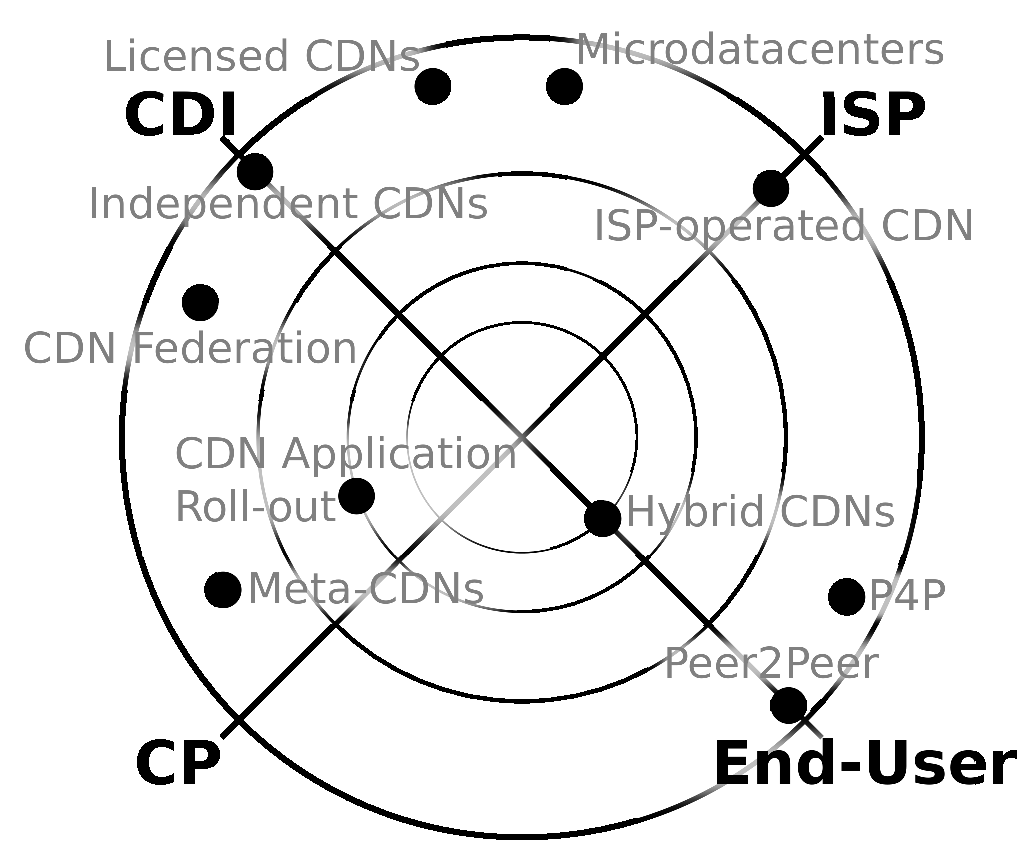
\includegraphics[width=0.7\linewidth]{figures-pdf/spectrum}
    \end{center}
    \caption{Spectrum of content delivery solutions and involvement of
      stake-holders in the content delivery. Reprinted from
      \cite{NetPaaS}. Included here by permission.}
    \label{fig:cdn-spectrum}
\end{figure}

\subsection{Independent Content Distribution}

Independent CDIs are usually referred to as Content Delivery Networks (CDNs).
They have a strong customer base of content producers and are responsible for
delivering the content of their customers to end-users around the world.
Today, they are, by traffic volume as well as hosted content, the largest
players on the Internet. In general, there are four main components to
independent CDN architectures: a server deployment, a strategy for replicating
content on servers, a mechanism for directing users to servers, and a system
for collecting and processing server logs.

For server deployment, three main approaches
exist~\cite{ImprovingPerformanceInternet2009}: centralized, datacenter based
and distributed infrastructures:

\textbf{Central Location}: This approach is used by small CDNs, One-Click
Hosters, and applications running in public clouds. Centralized hosting takes
advantage of (a) the economies of scale that a single location offers~
\cite{aboveclouds}, (b) the flexibility that multihoming
offers~\cite{Optimizing:Goldenberg2004}, and (c) the connectivity opportunities
that IXPs offer~\cite{IXPSIGCOMM2012}. The disadvantages of centralized hosting
are the potential for a single point of failure, and the limited ability to
ensure low latency to users located in different networks around the
world~\cite {CloudCmp}.

\textbf{Datacenter Based}: This approach deploys in several large data centers.
It again leverages economies of scale while improving reliability and creating
a larger footprint with further reach. However, by utilizing multiple
datacenters, new challenges regarding the content distribution, synchronization
and delivery arise. For example, the datacenter delivering content to an
end-user cannot be statically configured anymore, but the selection needs to
take the location of the end-user into account. This approach is used by CDNs
such as Limelight, EdgeCast and BitGravity. Many cloud providers also use this
approach, including Amazon CloudFront and Microsoft Azure.

\textbf{Distributed Infrastructures}: This approach consists of a highly
distributed infrastructure deployment, potentially deep inside third-party
networks. Here, the large number of servers scattered across numerous networks
offer high availability and replication of content while being very close to
end-users. Furthermore, this type can balance traffic across locations, best
react to flash crowds by dynamic server assignments, and deliver content with
improved latency. However, with the highly distributed infrastructures, the
challenges of assigning users to the right server location increase many-fold.
Also, with deep deployment datacenters are usually not available anymore,
leading to the question where to deploy how many servers. Today, Akamai is only
one independent CDN that uses this approach on a global scale.

\vspace{0.5em} CDNs with more than one location typically follow a pull
strategy~\cite{Akamai-Network} for content distribution and replication. Thus,
content requests can be directed to servers that do not have the required
object cached.  When a requested object is not at the selected server,
neighboring servers in the same cluster or region are asked. If the object is
not available at neighboring servers, the origin or root server responsible for
the object is contacted to retrieve the content. A requested object that is
fetched from a remote server is saved locally and then delivered to the end
user. To keep the copies of the object fresh, a TTL value is assigned to it.
When the TTL value expires, the object is removed. For scalability reasons, any
server of the CDN or within a region can respond to the request of an end
user~\cite{CDNsec2009}.

A special case of the independent CDI category are free CDNs such as
Coral~\cite{CoralCDN}, which follow a similar architectural design. In these
CDNs, server resources are offered by end-users or non-profit organizations.

\subsection{ISP-operated CDIs} The potential for generating revenue from
content delivery has motivated a number of ISPs to build and operate their own
Content Distribution Infrastructures. For example, large ISPs such as AT\&T and
Verizon have built their own CDNs along the same general architectural
principles as independent CDIs. However, due to the limitations arising from
being restricted to one network, these CDNs are not deployed in a distributed
fashion across multiple networks and thus are not globally operating solutions.
To overcome this issue, the CDNi group at the IETF~\cite {CDNi} is discussing
how to interconnect these CDNs to boost their efficiency and coverage. The
content provider are third parties, applications and services offered by the
ISP. Other ISPs with large footprints, such as Level3 and Telefonica~ \cite
{interdatacenter,ToN-DTB}, have also built CDNs in order to efficiently
transfer content across the globe and offer improved services to their end
users.

\subsection{Emerging Trends in CDI Architectures} Economics, especially cost
reduction, is the key driving force behind emerging CDI architectures. The
content delivery market has become highly competitive. While the demand for
content delivery services is rising and the cost of bandwidth is decreasing,
the profit margins of storage and processing \cite{aboveclouds} are dwindling,
increasing the pressure on CDIs to reduce costs. At the same time, more parties
are entering the market in new ways, looking to capture a slice of the revenue.
However, today's traditional CDI deployments lack agility to combat these
effects.  Contracts for server deployments last for months or years and the
available locations are typically limited to datacenters. The time required to
install a new server today is in the order of weeks or months. Such timescales
are too large to react to changes in demand. CDIs are therefore looking for new
ways to expand or shrink their capacity, on demand, and especially at low cost.

\subsubsection{Hybrid Content Distribution} In a hybrid CDI, end-users download
client software that assists with content distribution. As in P2P file-sharing
systems, the content is broken into pieces and offered by both other users who
have installed the client software as well as by the CDI's servers. The client
software contacts dedicated CDI servers, called control plane servers, which
schedule which parts of the content are to be downloaded from what peers.
Criteria for selecting peers include AS-level proximity as well as the
availability of the content. If no close peers are found, or if the download
process from other peers significantly slows the content delivery process, the
traditional CDI servers take over the content delivery job entirely. Akamai
already offers NetSession~\cite{HybridCDN-Bruce}, a hybrid CDI solution for
delivering very large files such as software updates at lower cost to its
customers.  Xunlei~\cite{Xunlei}, an application aggregator with high
penetration in China, follows a similar paradigm.  It is used to download
various types of files including videos, executables, and even emails, and
supports popular protocols such as HTTP, FTP, and RTSP.  Xunlei maintains its
own trackers and servers. A study of hybrid CDIs~\cite{HybridCDN-Ross} showed
that up to 80\% of content delivery traffic can be outsourced from server-based
delivery to end-users, without significant degradation in total download time.

\subsubsection{Licensed CDNs} Licensed CDNs have been proposed to combine the
benefits of the large content-provider customer base of an independent CDI with
the end-user base of an ISP~\cite{LicensedCDN}.  A licensed CDN is a
partnership between an independent CDI and an ISP. The CDI licenses the content
delivery software that runs on servers to the ISP while the ISP owns and
operates the servers. The servers deliver content to the end-users and report
logging information back to the CDI.  The revenue derived from content
producers is then shared between the two parties. Thus, a CDI can expand its
footprint deep inside an ISP network without investing in hardware, incurring
lower operating costs.  The ISP benefits from not having to invest in
developing the software for a reliable and scalable content distribution. More
importantly, a licensed CDN also alleviates the ISP's need to negotiate
directly with content producers, which might be challenging, given an ISPs
limited footprint.

\subsubsection{Application-based CDIs} Recently, large application and content
producers have rolled out their own CDIs, hosted in multiple large data
centers. Some popular applications generate so much traffic that the content
producers can better amortize delivery costs by doing content distribution
themselves.  Google is one such example.  It has deployed a number of data
centers and interconnected them with high speed backbone networks.  Google
connects its datacenters to a large number of ISPs via IXPs and also via
private peering.  Google has also launched the Google Global Cache
(GGC)~\cite{GoogleCache}, which can be installed inside ISP networks.  The GGC
reduces the transit cost of small ISPs and those that are located in areas with
limited connectivity, \eg Africa. The GGC servers are given for free to the
ISPs which install and maintain them.  GGC also allows an ISP to advertise
through BGP the prefixes of users that each GGC server should serve.  As
another example, Netflix, which is responsible for around 30\% of the traffic
in North America at certain times, is also rolling out its own CDI. The Netflix
system is called Open Connect Network~\cite{NetflixCDN}. Netflix offers an
interface where ISPs can advertise, via BGP, their preferences as to which
subnets are served by which Open Connect Network servers.

\subsubsection{Meta-CDIs} Today, content producers contract with multiple CDIs
to deliver their content.  To optimize for cost and
performance~\cite{Optimizing:SIGCOMM2012}, meta-CDIs act as brokers to help
with CDI selection. These brokers collect performance metrics from a number of
end-users and try to estimate the best CDI, based on the server that a user is
assigned. To this end, the brokers place a small file on a number of CDIs. Then
they embed the request for this file in popular websites' source code, in the
form of a javascript. When users visit these sites, they report back statistics
based on the servers that each CDI assigned the users. The broker then
recommends CDIs for a given source of demand taking also into consideration the
cost of delivery. Cedexis is one of these brokers for web browsing.  Another
broker for video streaming is Conviva~\cite{Conviva2011}. These brokers may
compensate when a CDI does not assign a user to the optimal server (which a
recent study~\cite{PADIS2010} has shown sometimes occurs) by selecting a
different CDI.


\subsubsection{CDI Federations} To avoid the cost of providing a global
footprint and perhaps to allow for a single negotiating unit with content
providers, federations of CDIs have been proposed. In this architecture,
smaller CDIs, perhaps operated by ISPs, join together to form a larger
federated CDI.  A CDI belonging to the federation can replicate content to a
partner CDI in a location where it has no footprint.  The CDI reduces its
transit costs because it only has to send the object once to satisfy the demand
for users in that location. Overall, cost may be reduced due to distance-based
pricing~\cite{HowManyTiers}. The IETF CDNi working group \cite{CDNi} works on
CDI federation.


%
%\newpage
\section{Challenges in Content Delivery}\label{sec:challenges}

The challenges that CDIs and P2P systems are faced with are based on the fact
that they are unaware of the underlying network infrastructure and its
conditions. In the best case, they can try to detect and infer the topology and
state of the ISP's network through measurements, but even with large scale
measurements, it is a difficult task, especially if accuracy is necessary.
Furthermore, when it comes to short-term congestion and/or avoiding network
bottlenecks, measurements are of no use. In the following we describe the
challenges those systems face in more detail.

\subsection{Content Delivery Infrastructures (CDIs)}\label{sec:CDIs-and-Challenges}

From the viewpoint of the end-users and ISPs, the redirection schemes employed
by existing CDIs have three major limitations:

\paragraph{Network Bottlenecks.} Despite the traffic flow optimization
performed by CDIs, the assignment of end-user requests to servers by CDIs may
still result in sub-optimal content delivery performance for the end-users.
This is a consequence of the limited information CDIs have about the network
conditions between the end-user and their servers. Tracking the ever changing
conditions in networks, \ie through active measurements and end-user reports,
incurs an overhead for the CDI without a guarantee of performance improvements
for the end-user.  Without sufficient information about the network paths
between the CDI servers and the end-user, any assignment performed by the CDI
may lead to additional load on existing network bottlenecks, or to the creation
of new bottlenecks.


\paragraph{User Mis-location.} DNS requests received by the CDI DNS servers
originate from the DNS resolver of the end-user, not from the end-user itself.
The assignment is therefore based on the assumption that end-users are close to
their DNS resolvers. Recent studies have shown that in many cases this
assumption does not hold~\cite {Precise:Mao2002,DNS-IMC-2010}. As a result, the
end-user is mis-located and the server assignment is not optimal. As a response
to this issue, DNS extensions have been proposed to include the end-user IP
information~ \cite{DNS-extension-IP-client}.  \paragraph{Content Delivery Cost}
Finally, CDIs strive to minimize the overall cost of delivering huge amounts of
content to end-users. To that end, their assignment strategy is mainly driven
by economic aspects.  While a CDI will always try to assign users in such a way
that the server can deliver reasonable performance, this can again result in
end-users not being directed to the server able to deliver best performance.

\subsection{Peer-to-Peer Networks (P2P)}\label{sec:P2P-and-Challenges}

P2P traffic often starves other applications like Web traffic of
bandwidth~\cite{swxzz-hptp-07}.  This is because most P2P systems rely on
application layer routing based on an overlay topology on top of the Internet,
which is largely independent of the Internet routing and
topology~\cite{abfw-mendg-04}. This can result in a situation where a node in
Frankfurt downloads a large content file from a node in Sydney, while the same
information may be available at a node in Berlin.  As a result P2P systems use
more network resources due to traffic crossing the underlying network multiple
times. For more details and information on P2P systems, see
Section~\ref{sec:P2P}.


\subsection{Internet Service Providers (ISPs)}\label{sec:ISPs-and-Challenges}

ISPs face several challenges regarding the operation of their network
infrastructure. With the emergence of Content, and especially distributed
content delivery, be it from CDIs or P2P networks, these operational challenges
have increased manifold.

\paragraph{Network Provisioning.} Provisioning and operation a network means
running the infrastructure at its highest efficiency. To ensure this, new
cables as well as the peering points with other networks need to be established
and/or upgraded. However, with the emergence of CDIs and P2P networks, the
network provisioning has become more complicated, since the network loads tend
to shift depending on the content that is currently transported while the
direct peering might not be effective anymore.

\paragraph{Volatile Content Traffic.} CDIs and P2P networks strive to optimize
their own operational overhead, possibly at the expense of the underlying
infrastructure. In terms of CDIs, this means that a CDI chooses the best server
based on its own criteria, not knowing what parts of the networks
infrastructure is being used. Especially with globally deployed CDIs it becomes
increasingly difficult for ISPs to predict what CDI is causing what traffic
from where based on past behavior. This has a direct implication on the traffic
engineering of the network, as this is usually based on traffic predictions
from past network traffic patterns.

\paragraph{Customer Satisfaction.} Regardless of the increased difficulty with
network provisioning and traffic engineering, end-users are demanding more and
larger content. This, coupled with the dominant form of flat rates for customer
subscriptions, increases the pressure on ISPs to delay network upgrades as long
as possible to keep prices competitive. But letting links run full increases
packet loss. This, in turn, drastically reduces the quality of experience of
the end-users. This, in turn, encourages end-users to switch their
subscriptions.


\subsection{Summary}

In summary, we identify the following challenges in todays content delivery:

\begin{itemize*}

\item The ISP has limited ability to manage its traffic and therefore incurs
  potentially increased costs, e.g., for its interdomain traffic, as well as
  for its inability to do traffic engineering on its internal network while
  having to offer competitive subscriptions to its end-users.

\item The P2P system has limited ability to pick an optimal overlay topology
  and therefore provide optimal performance to its users, as it has no prior
  knowledge of the underlying Internet topology. It therefore has to either
  disregard or reverse engineer it.

\item The CDI has limited ability to pick the optimal server and therefore
  provide optimal performance to its users, as it has to infer the network
  topology as well as the dynamic network conditions. Moreover, it has limited
  knowledge about the location of the user as it only knows the IP address of
  the DNS resolver.

\item The different systems try to measure the path performance independently.

\end{itemize*}

%
%\newpage
%%%%%%%%%%%%%%%%%%%%%%%%%%%%%%%%%%%%%%%%%%%%%%%%%%%%%%%%%%%%%%%%%%
\section{Incentives for Collaboration}\label{sec:Incentives}
%%%%%%%%%%%%%%%%%%%%%%%%%%%%%%%%%%%%%%%%%%%%%%%%%%%%%%%%%%%%%%%%%%

ISPs are in a unique position to help CDIs and P2P systems to improve content
delivery.  Specifically, ISPs have the knowledge about the state of the
underlying network topology and the status of individual links that CDIs are
lacking. This information not only helps CDIs in their user-to-server mapping,
but also reduces the need for CDIs to perform large-scale active measurements
and topology discovery \cite{sureroute}.  It also enables CDIs to better
amortize their existing infrastructure, offer better quality of experience to
their users, and plan their infrastructure expansion more efficiently. On the
other side, ISPs are not just selflessly giving up their network information.
Offering their intimate knowledge of the network to CDIs puts ISPs in the
position that they can also actively guide the CDIs. This allows ISPs to gain
unprecedented influence on CDI traffic.

The opportunity for ISPs to coordinate with CDIs is technically possible
thanks to the decoupling of server selection from content delivery. In general,
any end-user requesting content from a CDI first does a mapping request,
usually through the Domain Name System (DNS). During this request, the CDI
needs to locate the network position of the end-user and assign a server
capable of delivering the content, preferably close to the end-user.  ISPs have
this information ready at their fingertips, but are currently not able to
communicate their knowledge to CDIs. Furthermore, ISPs solve the challenge of
predicting CDI traffic, which is very difficult due to the lack of information
on the CDI mapping strategy regarding the end-users to servers assignment. In
order to reap the benefits of the other's knowledge, both parties require
incentives to work together.

\subsection{Incentives for CDIs}

The CDIs' market requires them to enable new applications while reducing
their operational costs and improve end-user experience~\cite{Akamai-Network}.
By cooperating with an ISP, a CDI improves the mapping of end-users to servers,
improves in the end-user experience, has accurate and up-to-date knowledge of
the networks and thus gains a competitive advantage. This is particularly
important for CDIs in light of the commoditization of the content delivery
market and the selection offered to end-users, for example through
meta-CDNs~\cite{Conviva2011}. The improved mapping also yields better
infrastructure amortization and, thanks to cooperation with ISPs, CDIs will no
longer have to perform and analyze voluminous measurements in order to infer
the network conditions or end-user locations.

To stimulate cooperation, ISPs can operate and provide their network
knowledge as a free service to CDIs or even offer discounts on peering or
hosting prices, \eg for early adopters and CDIs willing to cooperate. The loss
of peering or hosting revenue is amortized with the benefits of a lower network
utilization, reduced investments in network capacity expansion and by taking
back some control over traffic within the network. Ma et al.~\cite
{CooperativeSettlement:ToN} have developed a methodology to estimate the prices
in such a cooperative scheme by utilizing the Shapley settlement mechanism.
Cooperation can also act as an enabler for CDIs and ISPs to jointly launch new
applications in a cost-effective way, for example traffic-intensive
applications such as the delivery of high definition video on-demand, or
real-time applications such as online games.

\subsection{Incentives for ISPs}\label{sec:ISP-Incentive} 

ISPs are interested in reducing their operational and infrastructure upgrade
costs, offering broadband services at competitive prices, and delivering the
best end-user experience possible. Due to network congestion during peak hour,
ISPs in North America have recently revisited the flat pricing model and some
have announced data caps to broadband services. A better management of traffic
in their networks allows them to offer higher data caps or even alleviate the
need to introduce them. From an ISP perspective, cooperation with a CDI offers
the possibility to do global traffic and peering management through an improved
awareness of traffic across the whole network. For example, peering agreements
with CDIs can offer cooperation in exchange for reduced costs to CDIs. This can
be an incentive for CDIs to peer with ISPs, and an additional revenue for an
ISP, as such reduced prices can attract additional peering customers.
Furthermore, collaboration with CDIs has the potential to reduce the
significant overhead due to the handling of customer complaints that often do
not stem from the operation of the ISP but the operation of CDIs~\cite
{ControllingDataCloud}. Through this, ISPs can identify and mitigate congestion
in content delivery, and react to short disturbances caused by an increased
demand of content from CDIs by communicating these incidents back directly to
the source.

\subsection{Effect on End-users}\label{sec:Users-Incentive} 

Collaboration between ISPs and CDIs in content delivery empowers end-users to
obtain the best possible quality of experience. As such, this creates an
incentive for end-users to support the adoption of collaboration by both ISPs
and CDIs. For example, an ISP can offer more attractive products, \ie higher
bandwidth or lower prices, since it is able to better manage the traffic inside
its network.  Also, thanks to better traffic engineering, ISPs can increase
data caps on their broadband offers, making the ISP more attractive to
end-users. Moreover, CDIs that are willing to jointly deliver content can offer
better quality of experience to end-users. This can even be done through
premium services offered by the CDI to its customers. For example, CDIs
delivering streaming services can offer higher quality videos to end-users
thanks to better server assignment and network engineering.

%
%\newpage
%%%%%%%%%%%%%%%%%%%%%%%%%%%%%%%%%%%%%%%%%%%%%%%%%%%%%%%%%%%%%%%%%%
\section{Opportunities for Collaboration}\label{sec:Opportunities}
%%%%%%%%%%%%%%%%%%%%%%%%%%%%%%%%%%%%%%%%%%%%%%%%%%%%%%%%%%%%%%%%%%

As pointed out ISPs are in a unique position to help CDIs and P2P systems to
improve content delivery since they have the knowledge about the state of the
underlying network topology, the status of individual links, as well as the
location of the user. In this section we first describe the high level concept
all existing solutions have in common and then continue by illustrating where
and why they differ in certain aspects.

The presented solutions include the original Oracle concept proposed by
Aggarwal et al~\cite{afs-cispp2pcip-ccr07}, P4P proposed by Xie et al.~\cite{p4p},
Ono proposed by Choffnes and Bustamante~\cite{taming} and PaDIS proposed by Poese
et al.~\cite{PaDIS-IC}. We also give an overview of the activities within the
IETF which have been fueled to some extend by the proposed systems discussed in
this section, namely ALTO and CDNi.

\subsection{Conceptual Design}\label{sec:Concept-Opportunties-Collaboration}

To overcome the challenges in Content Delivery, recall
section~\ref{sec:challenges}, various solutions have been proposed by the
research community. While they all differ in certain aspects, their basic idea
is the same: utilize available information about the network to make an
educated selection prior connecting to a service.  Following this idea, all of
the proposed solution employ the same basic conceptual design: the
\emph{management plane} is responsible for collecting up-to-date information
about the network while the \emph{control plane} acts as an interface to this
information for the application.\\

\noindent {\bf Management Plane: The Network Map.}
The systems management plane is responsible to collect up-to-date state network
information, such as network topology, routing information, link utilization
and other important metrics. This information is used to maintain an internal
map of the network representing the current state of the real network.  One
important aspect of this component is how the information about the network is
retrieved. The different implementations range from active measurements over
passive measurements to active participation in network management systems
(such as BGP). Another important aspect is the frequency in which the
information is collected. For certain information such as topology or routing
an immediate update is necessary to guarantee correct functioning of the
system, while others, such as link utilization or packet loss rates, only
degrade the quality of the system. Still other information, such as link
capacities or transmission delays, can be considered (semi-)static.  Last but
not least the systems differ in what information is necessary to be
operational and if additional information sources can be used to improve
accuracy.\\

\noindent {\bf Control Plane: The Information Interface.}
The control plane of the system is responsible for providing an interface to
the information of the management plane so that clients can make use of the
information. This can basically be seen as an interface or API that clients can
query to get information about the current network state. The various proposed
solutions differ mainly in which fashion and at which granularity the
information can be retrieved. There are two main competing approaches:
abstracted network maps and preference lists. The first one transforms the
available information from the management plane into an annotated
representation of nodes and edges. The big difference to the actual data of the
management plane is the aggregation level and the specific annotations. Clients
can then query the system to get an up-to-date abstract network map, which they
can use to decide which of the possible destination to connect to by
calculating the best candidates by themselves using their own optimization
target. The second one uses the information of the management plane to create a
ranked list of possible service destinations (read: IP addresses). The required
input includes the source, possible destinations and (if the system supports
multiple collaboration objectives) an optimization goal, \eg minimal delay. The
output consists of a re-ordered list of the possible destinations in regard to
the optimization goal, the first being the most and the last being the least
desirable destination.

Note that in both cases the client is in the position to select the final
destination, allowing to completely ignore the additional information. Another
important fact is that the client is not necessarily the end-user but might be
a service provider themselves. For instance a company providing content
delivery service (CDN) could make use of this service to improve its
user-to-server mapping accuracy or in case of the BitTorrent P2P system the
tracker could query the service prior returning an initial peer list to a
connected client.  While not strictly necessary, the two components are
usually implemented as separate entities within the system to allow better
scalability, information aggregation and/or anonymization without loosing
precision or multiple collaboration objectives. In addition to that, all
systems table important issues for any collaboration approach, such as privacy
information leakage or targeted objective(s).

The presentation of the following solutions will outline the specific
implementation and thus highlights the differences between the solutions.

\subsection{P2P Oracle Service}\label{sec:p2p-collaboration}

Aggarwal et al.~\cite{afs-cispp2pcip-ccr07} describe an \emph{oracle} service to
solve the mismatch between the overlay network and underlay routing network in
P2P content delivery. Instead of the P2P node choosing neighbors independently,
the ISP can offer a service, the \emph{oracle}, that ranks the potential
neighbors according to certain metrics: a client supplied peer list is
re-ordered based on coarse-grained distance metrics, \eg the number of AS
hops~\cite{routing-book-00}, the peer being inside/outside the AS or the
distance to the edge of the AS. This ranking can be seen as the ISP expressing
preference for certain P2P neighbors.  For peers inside the network additional
information can be used, such as access bandwidth, expected delay or link
congestion to further improve the traffic management.


\subsection{Proactive Network Provider Participation for P2P (P4P)}\label{sec:P4P}

The ``Proactive Network Provider Participation for P2P'' is another approach to
enable cooperative network information sharing between the network provider and
applications. The P4P architecture~\cite{p4p} introduces iTrackers as portals
operated by network providers that divides the traffic control responsibilities
between providers and applications. Each iTracker maintains an internal
representation of the network in the form of nodes and annotated edges.  A node
represents a set of clients that can be aggregated at different levels, \eg
certain locations (PoP) or network state (similar level of congestion).
Clients can query the iTracker to obtain the ``virtual'' cost for possible peer
candidates. This ``virtual'' cost allows the network operators to express any
kind of preferences and may be based on the provider's choice of metrics,
including utilization, transit costs, or geography. It also enables the client
to compare and choose the most suited peers to connect to.


\subsection{Ono - Travelocity-based Path Selection}\label{sec:Ono}

The Ono system~\cite{taming} by Choffnes and Bustamante is based on
``techniques for inferring and exploiting the network measurements performed by
CDNs for the purpose of locating and utilizing quality Internet paths without
performing extensive path probing or monitoring'' proposed by Su \etal
in~\cite{DraftingAkamai:SIGCOMM2006}. Based on their observations that CDN
redirection is driven primarily by latency~\cite{DraftingAkamai:SIGCOMM2006},
they formulate the following hypothesis: Peers that exhibit similar redirection
behavior of the same CDN are most likely close to each other, probably even in
the same AS.  For this each peer performs periodic DNS lookups on popular CDN
names and calculates how close other peers are by determining the cosine
similarity with their lookups. To share the lookup among the peers they use
either direct communication between Ono enabled peers or via distributed
storage solutions \eg DHT-based.  On the downside Ono relies on the precision
of the measurements that the CDNs perform and that their assignment strategy is
actually based mainly on delay. Should the CDNs change their strategy in that
regard Ono might yield wrong input for the biased peer selection the authors
envision.

When considering our design concept described above, Ono is a bit harder to fit
into the picture: Ono distributes the functionality of the management and
control planes among all participating peers.  Also, Ono does not try to
measure the network state directly, but infers it by observing Akamai's
user-to-server mapping behavior on a large scale and relies on Akamai doing the
actual measurements~\cite{Akamai-Network}, Thus the management plane of Ono
consists of recently resolved hostnames from many P2P clients. The quality of
other peers can then be assessed by the number of hostnames that resolve to the
same destination.  The control plane in Ono's case is a DHT, which allows
decentralized reads and writes of key-value pairs in a distributed manner, thus
giving access to the data of the management plane.

\subsection{Provider-aided Distance Information System (PaDIS)}\label{PaDIS-Opportunities-for-Collaboration}
\newcommand{\assignmentenabler}{{informed user-server as\-sign\-ment}\xspace}
\newcommand{\assignment}{{user-server as\-sign\-ment}\xspace}
\newcommand{\assignmentproblem}{{informed user-server as\-sign\-ment problem}\xspace}


In~\cite{PADIS2010,PaDIS-IC} Poese et al. propose a ``Provider-aided Information Systems
(PaDIS)'', a system to enable collaboration between network operators and
content delivery systems. The system enhances concept of the P2P Oracle to
include server based content delivery systems (\eg CDNs), to maintain an
up-to-date annotated map of the ISP network and its properties as well as the
state of ISP-operated servers that are open for rent. In addition, it provides
recommendations on possible locations for servers to better satisfy the demand
by the CDN and ISP traffic engineering goals.  In the management plane, it
gathers detailed information about the network topology, \ie routers and links,
annotations such as link utilization, router load as well as topological
changes. An Interior Gateway Protocol (IGP) listener provides up-to-date
information about routers and links.  Additional information, \eg link
utilization and other metrics can be retrieved via SNMP. A Border Gateway
Protocol (BGP) listener collects routing information to calculate the paths
that traffic takes through the network, including egress traffic. Ingress
points of traffic can be found by utilizing Netflow data. This allows for
complete forward and reverse path mapping inside the ISP and enables a complete
path map between any two points in the ISP network.  While PaDIS builds an
anotated map of the ISP network, it keeps the information acquired from other
components in separate data structures. This separation ensures that changes in
prefix assignments do not directly affect the routing in the annotated network
map.  Pre-calculating path properties for all paths, allow for constant lookup
speed independent of path length and network topology. On the control plane,
PaDIS makes use of the prefrence lists known from the P2P Oracle, but supports
multiple, individual optimization targets. Apart from basic default
optimizations (\eg low delay, high throughput), additional optimizations can be
negotiated between the network operator and the content delivery system.
For CDN-ISP collaboration opportunities when the ISP operates both the network and the CDN we
refer the reader to~\cite{CooperativeISPCDN,TECDN,N-CDN,CTTE2010}.

\subsection{Application-Layer Traffic Optimization (ALTO)}\label{sec:ALTO}

The research into P2P traffic localization has led the IETF to form a working
group for ``Application Layer Traffic Optimization (ALTO)''~\cite{ALTO-WG}.
The goal of the ALTO WG is to develop Internet standards that offer
``better-than-random'' peer selection by providing information about the
underlying network and to design a query-response protocol that the
applications can query for an optimized peer selection
strategy~\cite{ietf-alto-protocol}.  On the control plane, ALTO offers multiple
services to the Applications querying it, most notably are the Endpoint Cost
Service and the Map service. The Endpoint Cost Service allows the Application
the query the ALTO server for costs and rankings based on endpoints (usually IP
subnets) and use that information for an optimized peer selection process or to
pick the most suitable server of a CDI. The Network Map service makes use of
the fact that most endpoints are in fact rather close to each other and thus
can be aggregated into a single entity. The resulting set of entities is then
called an ALTO Network Map. The definition of proximity in that case depends on
the aggregation level, in one Map endpoints in the same IP subnet may be
considered close while in another all subnets attached to the same Point of
Presence (PoP) are close. In contrast to the Endpoint Cost Service the ALTO
Network Map is suitable when more Endpoints need to be considered and offers
better scalability, especially when coupled with caching techniques. Although
the ALTO WG statement is more P2P centric, the service is also suitable to
improve the connection to CDN servers.


%
%\newpage
%%%%%%%%%%%%%%%%%%%%%%%%%%%%%%%%%%%%%%%%%%%%%%
\section{Collaboration Use Cases: P2P and TE}\label{sec:Oracle-and-TE}
%%%%%%%%%%%%%%%%%%%%%%%%%%%%%%%%%%%%%%%%%%%%%%

The growth of demand for content is motivating collaboration between ISPs and
applications. In this chapter we review to use cases: P2P and Traffic Engineering.

\subsection{Use Case: P2P}\label{sec:oracle} 

Recall, P2P systems are self-organizing systems of autonomous entities, called
peers, that cooperate for common goals. These common goals range from sharing
of resources, e.g., music and video files, processing power, or storage
space~\cite{P2P-LNCS-05} to collaborative routing as in Skype and P2P-TV.  A
fundamental characteristic of these systems is their distributed designs and
resources.

Advantages of P2P systems include elimination of bottlenecks and single
points-of-failure within the system, increased processing power, high
availability/redundancy, and little or no dependence on any particular central
entity.  However, P2P systems are plagued by some fundamental issues, such as
overlay/underlay topological and routing mismatch~\cite{sa-oidronl-06},
inefficiencies in locating and retrieving resources, and scalability and
performance issues caused by uncontrolled traffic swamps~\cite{P2P-LNCS-05}.

Several of these drawbacks can be addressed by collaboration between the P2P
overlay and the Internet routing underlay. To overcome these limits each ISP
can offer the ``oracle'' service as introduced in
Section~\ref{sec:p2p-collaboration} to the P2P users which explicitly helps P2P
users to choose ``good'' neighbors.  The P2P user can supply its ISP's oracle
with a list of possible P2P neighbors, during bootstrapping and/or content
exchange.  The ISP's oracle then returns a ranked list to the querying user,
according to its preference (\eg AS-hop distance) and knowledge of the ISP
topology and traffic volume, while at the same time keeping the interest of the
P2P user in mind.  We  show that in principle, P2P systems as well as the ISPs
profit from the use of the oracle even when only considering the AS-distance
for ranking nodes~\cite{afs-cispp2pcip-ccr07}, because the overlay topology is now
localized and respects the underlying Internet topology, and the P2P user
profits from the ISP's knowledge.

To study the impact of biased neighbor selection on a real P2P network that
implements its own routing, we run extensive simulations of the Gnutella
protocol. We show that in contrast to the unmodified P2P system, the ISP-aided
localized P2P system shows consistent improvements in the observed end-user
experience, measured in terms of content download times, network locality of
query responses and desired content, and quality of query responses. A
significantly large portion of P2P traffic remains local to the ISP network,
and ISPs notice a substantial reduction in overall P2P traffic. This can lead
to immense cost savings for the ISPs~\cite{Cachelogic}. The oracle consistently
shows performance gains even across different topologies under a broad range of
user behavior scenarios. For a more detailed analysis of the P2P oracle
service, see~\cite{afs-cispp2pcip-ccr07, af-ispabqsp2pt-eccs07,afk-icsecispp2p-icin07}.



\subsubsection{Influence on P2P Topology}\label{sec:Influence-Oracle-on-P2P-Topology}

To explore the influence of consulting the oracle on the network topology we
visualize, in Figure~\ref{fig:oracle:gnutella_topology}~\cite{tashev-thesis},
the Gnutella overlay topology. At a particular instant in time, we sample the
Gnutella overlay topology, display all the online nodes in the graph, and join
two nodes with an edge if there exists a Gnutella peering between them at this
point of time. The resulting graph structures are displayed in
Figure~\ref{fig:oracle:gnutella_topology}. For our simulations we consider $5$
different topologies: Germany, USA, World1, World2 and World3, each modeled
after their respective AS topologies (World1-3 differ in the size of the ASes).
We can easily observe that the Gnutella topology in the biased case is well
correlated with the Internet AS topology, where the nodes within an AS form a
dense cluster, with only a few connections going to nodes in other ASes. This
is in stark contrast to the unbiased Gnutella graph, where no such property can
be observed. Multiple runs of the above experiments, using the different
topologies yield similar results.

\begin{figure}[tbp]
   \begin{subfigure}[]{0.4\linewidth}
     {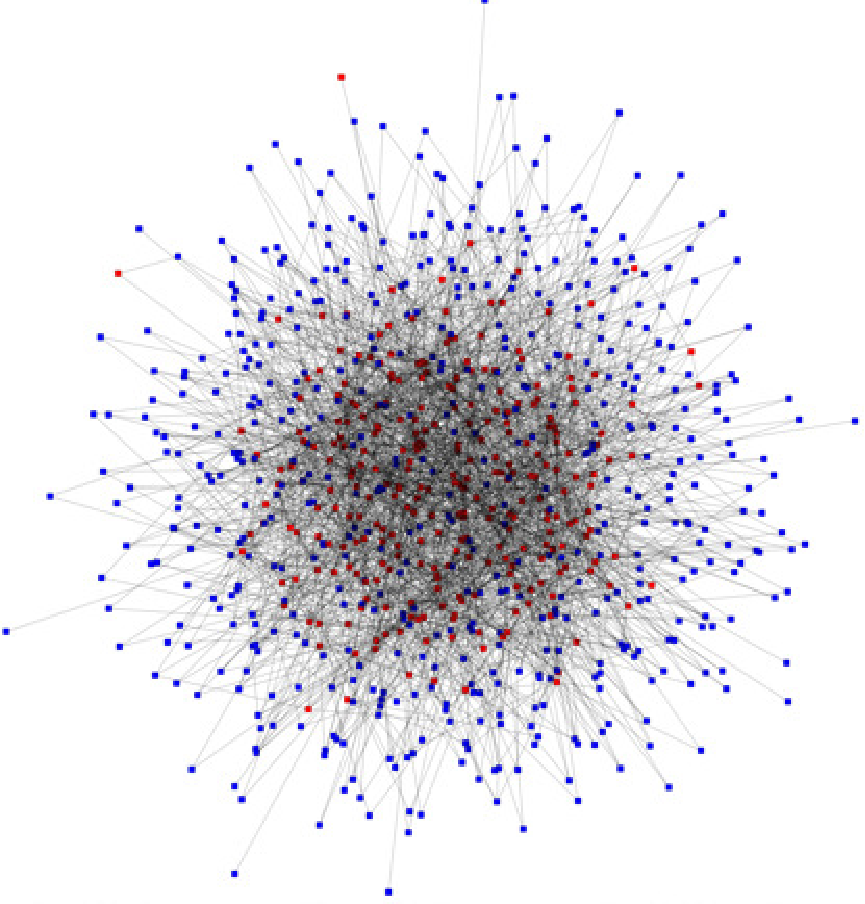
\includegraphics[angle=-90,width=1\linewidth]{figures-pdf/snapshot_nond}}
   \caption{Unbiased Gnutella}%
   \end{subfigure}
\hfill
   \begin{subfigure}[]{0.45\linewidth}
     {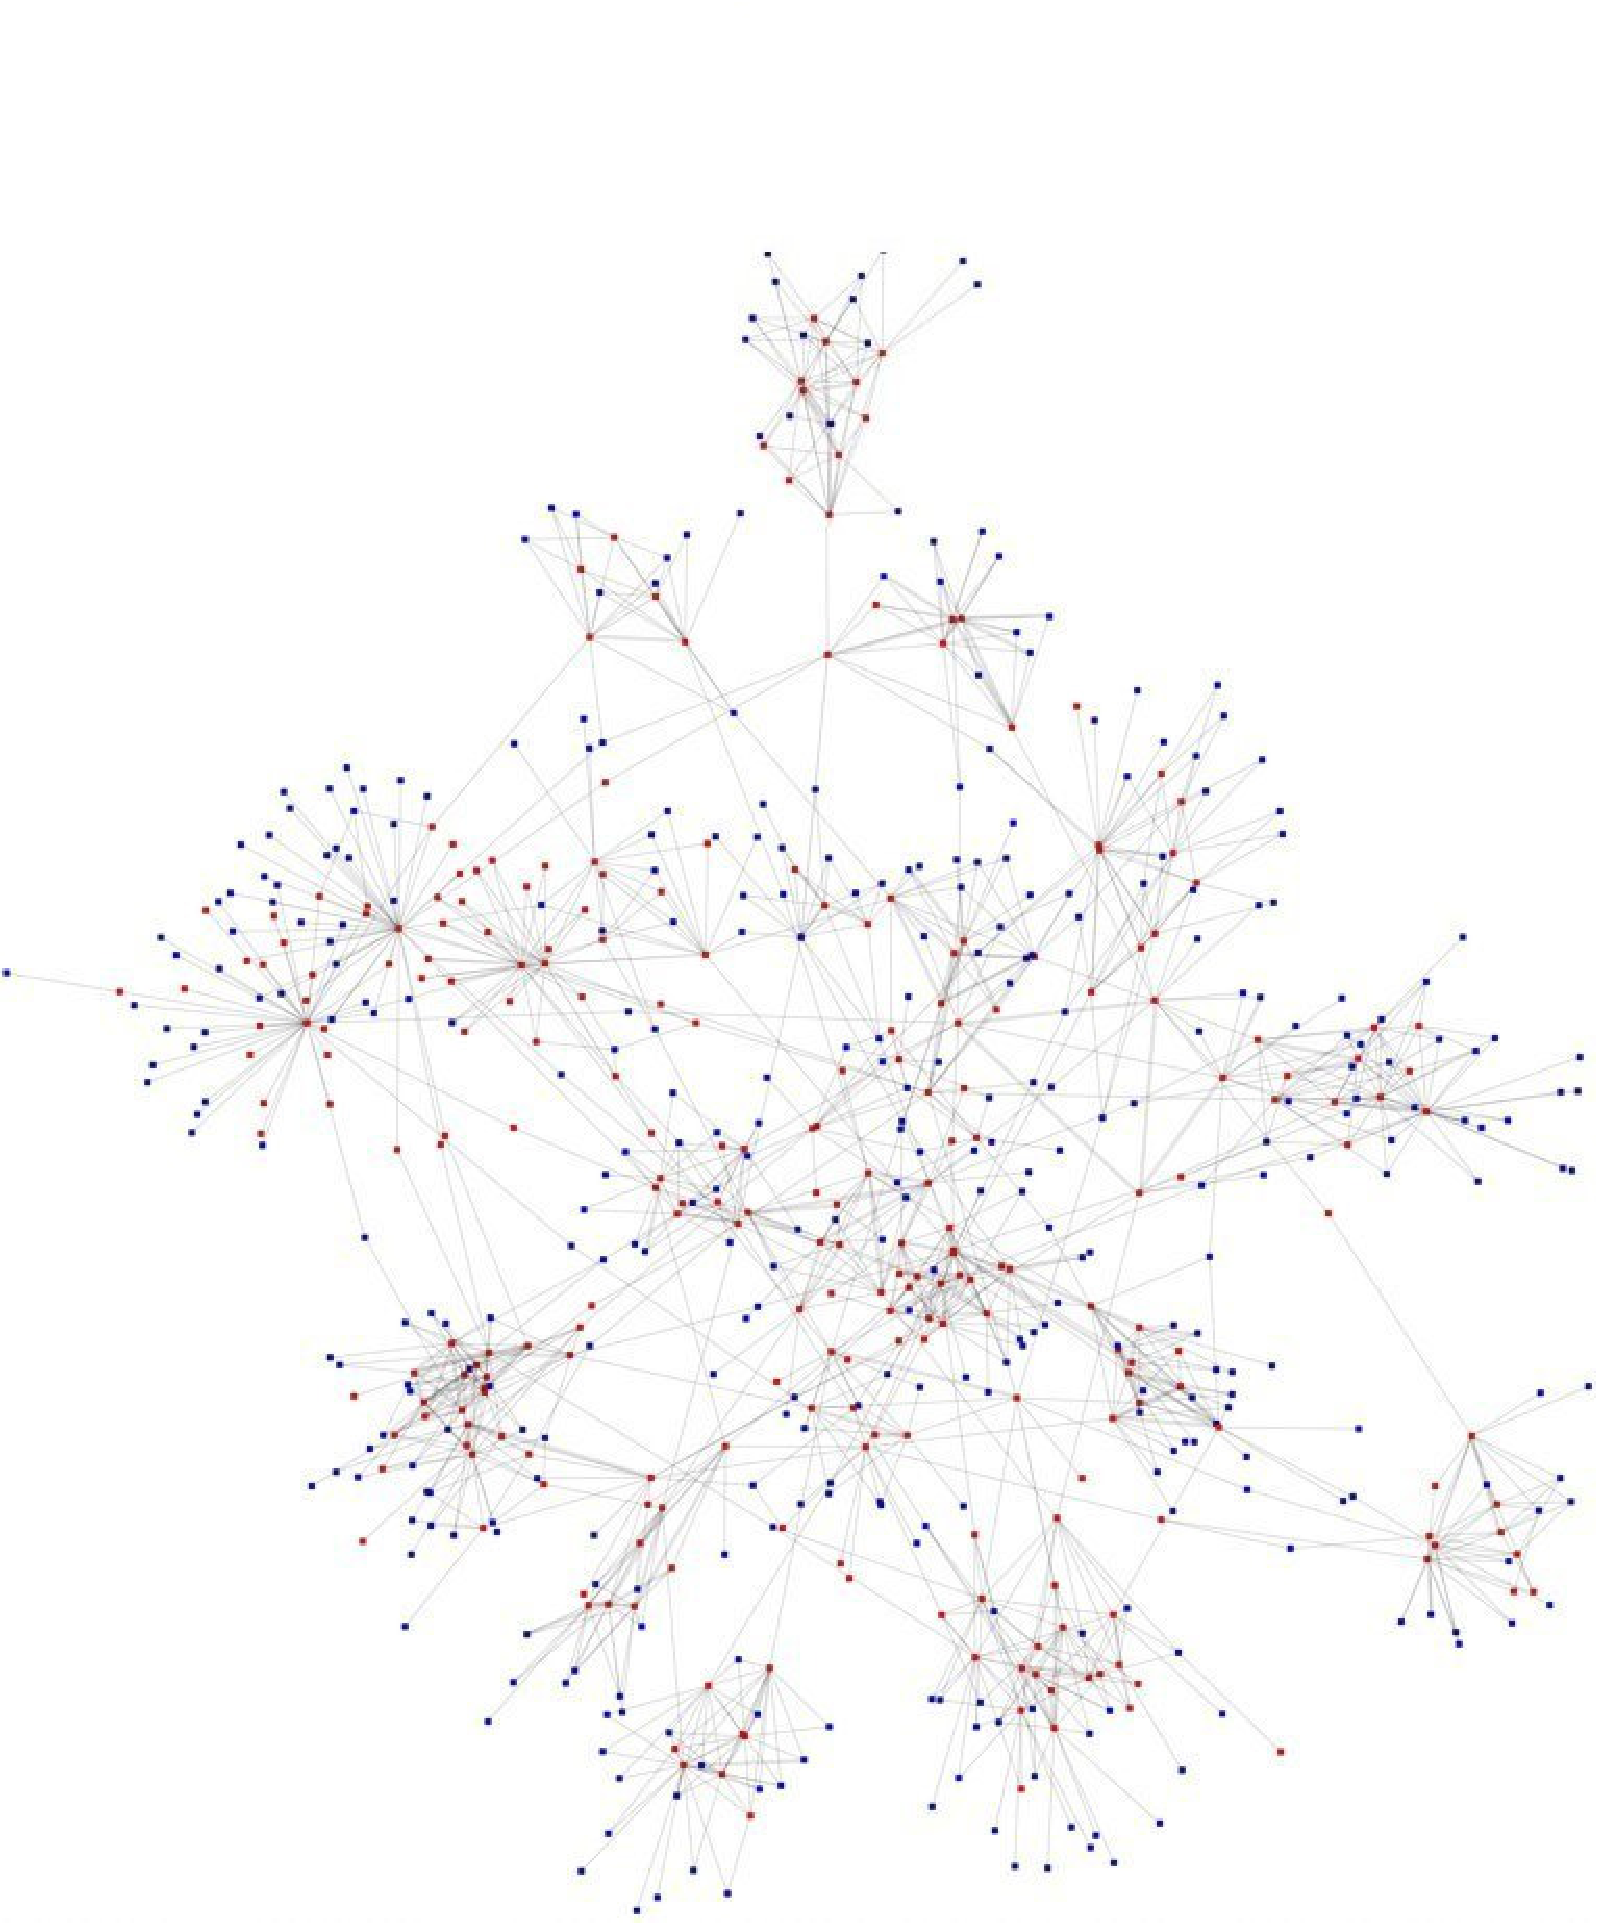
\includegraphics[angle=-90,width=1\linewidth]{figures-pdf/snapshot_nd}}
   \caption{Gnutella with Oracle}%
   \end{subfigure}   \caption{Visualization of Gnutella
     overlay topology. Reprinted from \cite{afs-cispp2pcip-ccr07}. Included here by permission.}
   \label{fig:oracle:gnutella_topology}
\end{figure}




\subsubsection{Benefits of Collaboration}\label{sec:Benefits-Collaboration-P2P-results}


\noindent\textbf{Mean AS distance:} \\
The benefits of using an oracle for biasing the neighborhood in Gnutella are visible in
Figure~\ref{fig:oracle:gnutella_metric:2a}, which shows the average AS distance (in the underlay)
between any two connected Gnutella nodes. The AS distance is obtained as follows. We map
each Gnutella node's IP address to its parent AS, and for each overlay edge, we find the
network distance in AS hops between the two end-nodes.  We observe that the least amount
of decrease in the average AS distance occurs from $1.93$ to $0.8$ at $1000$ seconds, and
the maximum decrease from $1.94$ to $0.25$ happens at $5000$ seconds. Given that the AS
diameter remains constant at $4$ hops, the average decrease of $1.45$ in the AS distance
is significant. Besides, as the average AS distance in the case of oracle list size of
$1000$ is $0.45$, a value less than $1$, it implies that most of the Gnutella peerings are
indeed within the ASes, i.e., they are not crossing AS boundaries. This can be a major
relief for ISPs, as they do not incur any additional cost for traffic within their
domains. Also traffic that does not leave the network is easier to manage. Moreover, P2P
traffic will not encounter inter-ISP bottlenecks.


\begin{figure}[tbp]
	\begin{subfigure}[]{0.32\linewidth}
     {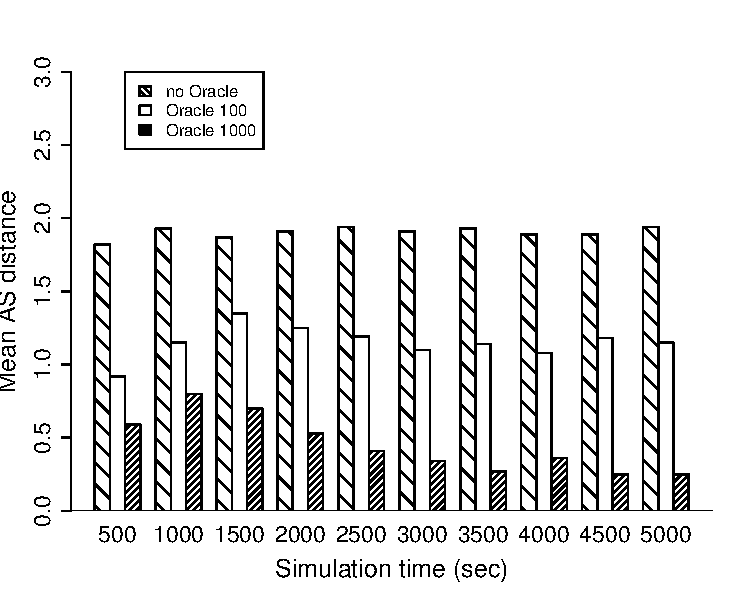
\includegraphics[width=1\textwidth]{figures-pdf/asdist}}
    \caption{Mean AS distance in Underlay\label{fig:oracle:gnutella_metric:2a}}
    \end{subfigure}
 \hfill
    \begin{subfigure}[]{0.32\linewidth}
    {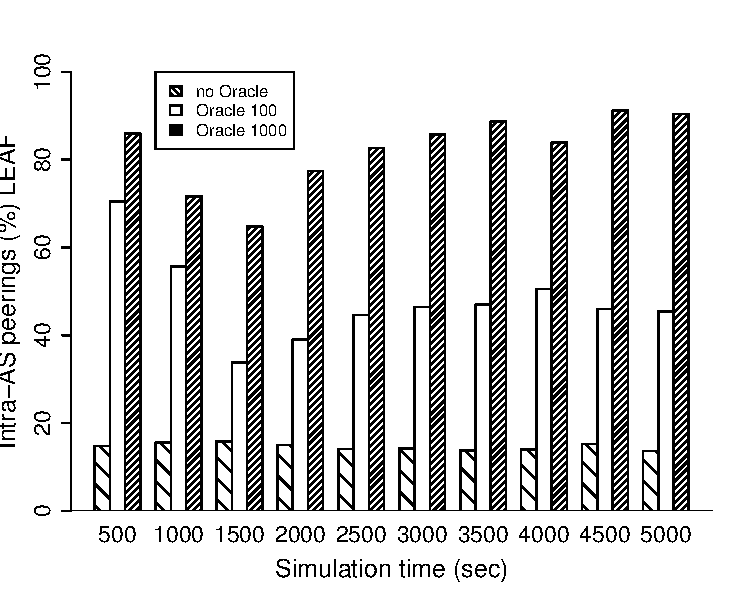
\includegraphics[width=1\textwidth]{figures-pdf/intraAS-leaf}}
    \caption{Intra-AS peerings (\%) for Leaf nodes\label{fig:oracle:gnutella_metric:2b}}
    \end{subfigure}
 \hfill
    \begin{subfigure}[]{0.32\linewidth}
    {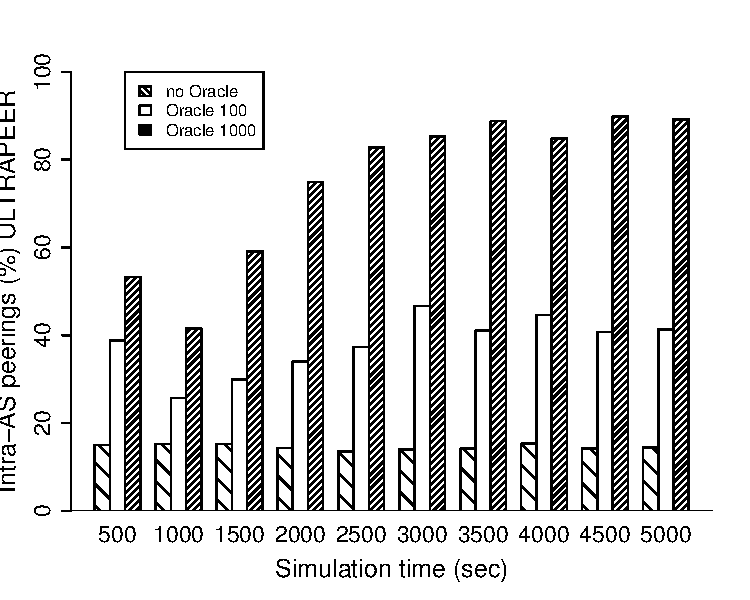
\includegraphics[width=1\textwidth]{figures-pdf/intraAS-up}}
    \caption{Intra-AS peerings (\%) for Ultrapeers\label{fig:oracle:gnutella_metric:2c}}
    \end{subfigure}
    \caption{Metrics for Gnutella simulations}
   \label{fig:oracle:gnutella_metric}
\end{figure}


\vspace{0.75\baselineskip}
\noindent\textbf{Intra-AS P2P connections:} \\
The above observations on AS distance are even better understood from the plots in
Figures~\ref{fig:oracle:gnutella_metric:2b} and \ref{fig:oracle:gnutella_metric:2c}, where we show the total number of intra-AS
P2P connections in the Gnutella network as a percentage of the total number of intra- and
inter-AS P2P connections, for both leafs and ultrapeers.

In Figure~\ref{fig:oracle:gnutella_metric:2b}, we observe that in the case of leaf nodes, taking
the average over the $10$ time points, the percentage of intra-AS P2P connections
increases from $14.6$\% in unbiased case to $47.88$\% in the case of oracle with list size
$100$. For oracle with list size $1000$, we note an average of $82.22$\% intra-AS P2P
connections.

In Figure~\ref{fig:oracle:gnutella_metric:2c}, we observe similar results for ultrapeers. The
percentage of intra-AS P2P connections increases from an average value of $14.54$\% in the
unbiased case to $38.04$\% in the case of oracle with list size $100$, and further to
$74.95$\% in case of oracle with list size $1000$.

The percentage increase in intra-AS P2P connections is larger for leaf nodes as compared
to ultrapeers, a welcome development.  One needs a certain number of inter-AS connections,
to maintain network connectivity and to be able to search for file content that may not be
available within an AS. However, as leaf nodes typically have poor connectivity to the
Internet, and have lower uptimes, it is reasonable to have leaf nodes keep most of their
peerings within their AS, while allowing the ultrapeers to have slightly more connections
outside their ASes.

For the impact of Oracle on download time under different topologies we refer
the reader to~\cite{improving-oracle-GI-2008}. For the impact of Oracle-like
localization techniques on the inter-AS traffic flow of the BitTorrent P2P
system we refer the reader to~\cite{DeepDiving,LocalityP2P,BlindMiceBT,Impact-Profitability}.


%%%%%%%%%%%%%%%%%%%%%%%%%%%%%%%%%%%%%%%%%%%%%%
\subsection{Use Case: Traffic Engineering}\label{sec:te-cate}
%%%%%%%%%%%%%%%%%%%%%%%%%%%%%%%%%%%%%%%%%%%%%%

The growth of demand for content and the resulting deployment of content
delivery infrastructures pose new challenges to CDIs and to ISPs. For CDIs, the
cost of deploying and maintaining such a massive infrastructure has
significantly increased during the last years~\cite{AkamaiCutting:2009} and the
revenue from delivering traffic to end-users has decreased due to the intense
competition. Furthermore, CDIs struggle to engineer and manage their
infrastructures, replicate content based on end-user demand, and assign users
to appropriate servers.

The latter is challenging as end-user to server assignment is based on
inaccurate end-user location
information~\cite{Precise:Mao2002,DNS-extension-IP-client}, and inferring the
network conditions within an ISP without direct information from the network is
difficult. Moreover, due to highly distributed server deployment and adaptive
server assignment, the traffic injected by CDIs is volatile. For example, if
one of its locations is overloaded, a CDI will re-assign end-users to other
locations, resulting in large traffic shifts in the ISP network within minutes.
Current traffic engineering by ISP networks adapts the routing and operates on
time scales of several hours, and is therefore too slow to react to rapid
traffic changes caused by CDIs.

The pressure for cost reduction and customer satisfaction that both CDIs and
ISPs are confronted with, coupled with the opportunity that distributed server
infrastructures offer, motivate us to propose a new tool in the traffic
engineering landscape. We introduce \emph{Content-aware Traffic Engineering}
(\cate). \cate leverages the location diversity offered by CDIs and, through
this, it allows to adapt to traffic demand shifts. In fact, \cate relies on the
observation that by selecting an appropriate server among those available to
deliver the content, the path of the traffic in the network can be influenced
in a desired way. Figure~\ref{fig:flowSelection} illustrates the basic concept
of \cate. The content requested by the client is in principle available from
three servers (A, B, and C) in the network. However, the client only connects
to one of the network locations. Today, the decision of where the client will
connect to is solely done by the CDI and is partially based on measurements
and/or inference of network information and end-user location. With \cate the
decision on end-user to server assignment can be done jointly between the CDI
and ISP.

\begin{figure}[tbp]
  \center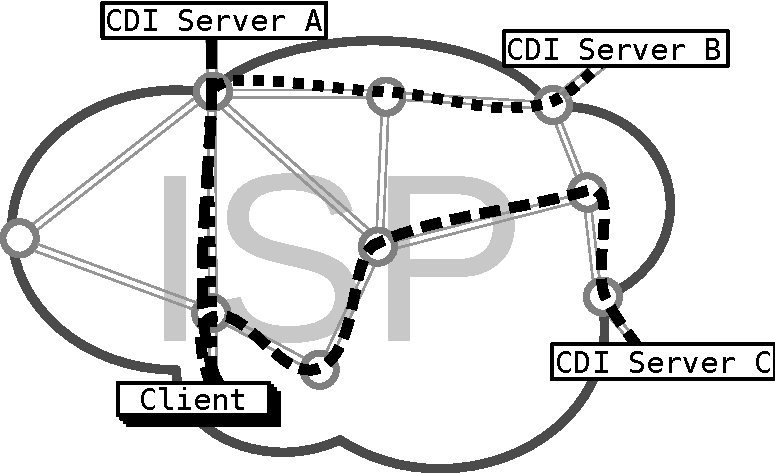
\includegraphics[width=0.8\linewidth]{figures-pdf/trafficShift-concept}
  \caption{By choosing a CDI server for a client with the help of CaTE, traffic
  engineering goals and accurate end-user server assignment become
  possible. Reprinted from \cite{Cate-CCR}. Included here by permission.}
  \label{fig:flowSelection}
  \vspace{-1.5em}
\end{figure}


%%%%
\subsubsection{The CaTE Approach}\label{sec:cate}
%%%%

\cate complements existing traffic engineering solutions
\cite{ietf-alto-protocol,TECDN,CooperativeISPCDN,BeyondMLU,CooperativeISPCDN:Workshop,p4p}
by focusing on traffic demands rather than routing.  Let {\bf y} be the vector
of traffic counts on links and {\bf x} the vector of traffic counts in
origin-destination (OD) flows in the ISP network.  Then {\bf y}=$A${\bf x},
where $A$ is the routing matrix. $A_{ij}=1$ if the OD flow $i$ traverses link
$j$ and $0$ otherwise.  Traditional traffic engineering is the process of
adjusting $A$, given the OD flows {\bf x}, so as to influence the link traffic
{\bf y} in a desirable way.  In \cate, we revisit traffic engineering by
focusing on traffic demands rather than routing changes. Content-aware Traffic
Engineering (\cate) is thus the process of adjusting the traffic demand vector
{\bf x}, without changing the routing matrix $A$, so as to change the link traffic {\bf y}
in a desirable way.

\cate offers additional traffic engineering capabilities to both ISPs and CDNs
to better manage the volatility of content demand in small time scales.
Traditional traffic engineering
\cite{ietf-alto-protocol,TECDN,CooperativeISPCDN,BeyondMLU,CooperativeISPCDN:Workshop,p4p}
relies on changes of routing weights that take place in the time scale of hours
\cite{FT01}.  On the contrary, in \cate, the redirection of end-users to servers can take place
per request or within the TTL of a DNS query that is typically tens of seconds
in large CDNs \cite{PADIS2010}.  Thanks to the online recommendations by ISP
networks, CDNs gain the ability to better assign end-users to servers and
better amortize the deployment and maintenance cost of their infrastructure.
Network bottlenecks are also circumvented and thus the ISP operation is
improved.  Furthermore, the burden of measuring and inferring network topology,
and the state of the network, both challenging problems, is removed from the
CDNs. Moreover, in \cite[Sections 4 and 5]{CaTE-TR} we show that the online
\cate decisions on the end-user to server assignment leads to optimal traffic
assignment within the network under a number of different metrics.  The
advantage is that now the problem of assigning traffic to links reduces to a
fractional solution (on the contrary, assigning routing weights to links is
NP-hard).  In short, all involved parties, including the end-users, benefit
from \cate, creating a win-win situation for everyone.




%%%%%%%%%%%%%%%%%%%%%%%%%%%%%%%
\subsubsection{A Prototype to Support CaTE}\label{sec:system}
%%%%%%%%%%%%%%%%%%%%%%%%%%%%%%%
\cate relies on a close collaboration between CDN and ISP in small time scales
(seconds or per request).  To achieve this goal, network information has to be
collected and processed by the ISP.  Candidate CDN servers have to be
communicated to the ISP and ranked based on a commonly agreed criteria, \eg to
optimize the delay between the end-user and the CDN server.  Today, there is no
system to support the above operations.  This motivate us to design, implement
and evaluate a novel and scalable system that can support \cate.  In this
section we describe the architecture and deployment of our working prototype to
enable \cate.  We start by presenting our prototype in
Section~\ref{sec:architecture}.  We then  comment on its operation and
deployment within the ISP, its interaction with a CDN, and its performance that
is beyond the state-of-the-art \cite{ietf-alto-protocol}.


%%%%%%%%%%%%%%%%%%%%%%%%%%%%%%%%%%%%%%%%%%%%%%%%%%%%%%%%
\ \\\noindent\textbf{Architecture:}\label{sec:architecture}\\\noindent
%%%%%%%%%%%%%%%%%%%%%%%%%%%%%%%%%%%%%%%%%%%%%%%%%%%%%%%
The \cate system is installed in an ISP and interacts with the existing CDN
server selector. The main tasks of the \cate system are to: (1) maintain an
up-to-date annotated map of the ISP network and its properties, (2) produce
preference rankings based on the paths between end-users and candidate servers,
and (3) communicate with the CDN server selection system to influence the
assignment of end-user to servers.  To this end, we propose an architecture
that comprises a {\it Network Monitoring} component, a {\it Query Processing}
component and a {\it communication interface} between an ISP and a CDN.  For an
overview of the architecture see Figure~\ref{fig:CaTE-architecture}.


%%%%%%%%%%%%%%%%%%%%%%%%%%%%%%%%%%%%%%%%%%%%%%%%%%%%%%%%
\ \\\noindent\textbf{Network Monitoring:}\label{sec:Network-monitoring}\\\noindent
%%%%%%%%%%%%%%%%%%%%%%%%%%%%%%%%%%%%%%%%%%%%%%%%%%%%%%%
The network monitoring component gathers information about the topology and the
state of the network from several sources to maintain an up-to-date view of the
network.  The network monitoring component consists of the following
subcomponents:

The {\bf Topology Information} component gathers detailed information about the
basic network topology, \ie routers and links, as well as annotations such as
link utilization, router load, and topological changes.  An Interior Gateway
Protocol (IGP) listener provides up-to-date link-state (\ie IS-IS, OSPF)
information.  Information about routers and links is retrieved, thus, the
network topology can be extracted.  The nominal link delay, \ie the latency on
a link without queuing, can be found through the link length and physical
technology.  The link utilization and other metrics can be retrieved via SNMP
from the routers or an SNMP aggregator.

The {\bf Connectivity Information} component uses routing information to
calculate the paths that traffic takes through the network. Finding the path of
egress traffic can be done by using a Border Gateway Protocol (BGP) listener.
Ingress points of traffic into the ISP network can be found by utilizing
Netflow data. This allows for complete forward and reverse path mapping inside
the ISP.  Furthermore, the system can map customers as well as CDN
infrastructures into the network map by finding the routers that announce the
address space associated with them. In total, this allows for a complete path
map between any two points in the ISP network.  Finally, our system has access
to an uplink database that provides information about the connectivity
statistics of end-users.


\begin{figure}[tbp]
    \center 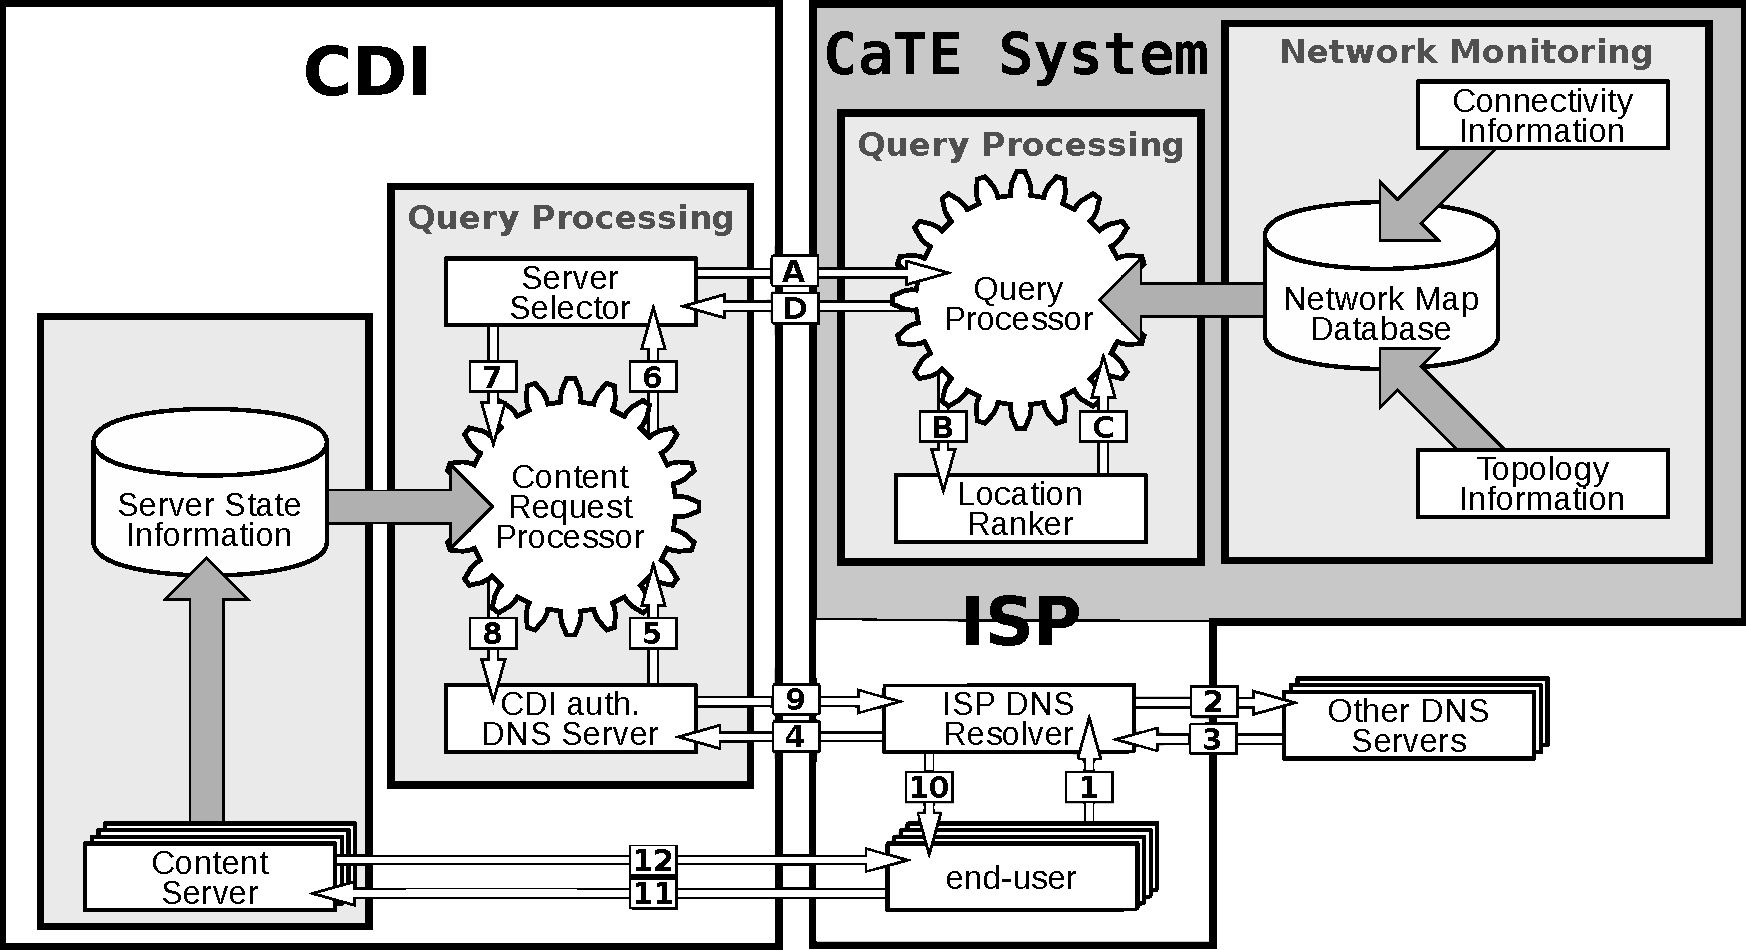
\includegraphics[width=3.2in]{figures-pdf/CaTE_Schematic}
  \vspace{-0.1in}
    \caption{CaTE System architecture and flow of messages. Reprinted from \cite{Cate-CCR}. Included here by permission.}
    \label{fig:CaTE-architecture}
    \vspace{-0.2in}
\end{figure}

The {\bf Network Map Database} component processes the information collected by
the {\it Topology} and {\it Connectivity Information} components to build an
annotated network map of the ISP network tailored towards fast lookup on path
properties.  It uses a layer of indirection to keep the more volatile
information learned from BGP separate from the slower changing topological
information.  This allows address space to be quickly reassigned without any
reprocessing of routing or path information.  It also enables pre-calculation
of path properties for all paths that yields a constant database lookup
complexity independent of path length and network architecture.  If topology
changes, \eg IGP weights change or a link fails, the {\it Topology Information}
component immediately updates the database which only recalculates the
properties of the affected paths.  Having ISP-centric information ready for
fast access in a database ensures timely responses and high query throughput.



%%%%%%%%%%%%%%%%%%%%%%%%%%%%%%%%%%%%%%%%%%%%%%%%%%%%%%%%
\ \\\noindent\textbf{Query Processing:}\label{sec:Query-Processing}\\\noindent
%%%%%%%%%%%%%%%%%%%%%%%%%%%%%%%%%%%%%%%%%%%%%%%%%%%%%%%
The {\bf Query Processing} component receives a description of a request for
content from the CDN, which specifies the end-user making the request and a
list of candidate CDN servers.  It then uses information from the {\it Network
  Map Database} and a selected ranking function to rank the candidate servers.
This component consists of the following subcomponents:

The {\bf Query Processor} receives the query from the CDN.  First, the query
processor maps each source-destination (server to end-user) pair to a path in
the network.  In most cases, the end-user is seen as the ISP DNS resolver,
unless both ISP and CDN support the client IP eDNS
extension~\cite{DNS-extension-IP-client}.  Once the path is found, the
properties of the path are retrieved. Next, the pairs are run individually
through the location ranker subcomponent (see below) to get a preference value.
Finally, the list is sorted by preference values, the values are stripped from
the list, and it is sent back to the CDN.

The {\bf Location Ranker} component computes the preference value for
individual source-destination pairs based on the source-destina\-tion path
properties and an appropriate function.  Which function to use depends on (a)
the CDN, (b) what metrics the CDN asked for and (c) the optimization goal of
the ISP.  The preference value for each source-destination pair is then handed
back to the Query Processor.  Multiple such optimization functions being
defined upon the collaboration agreement and subsequently selected individually
in each ranking request. For example, a function might be the minimization of
end-user and server delay.  In~\cite{CaTE-TR} we evaluate \cate
with multiple ranking functions for different optimization goals.


%%%%%%%%%%%%%%%%%%%%%%%%%%%%%%%%%%%%%%%%%%%%%%%%%%%%%%%%
\ \\\noindent\textbf{Communication Interfaces:}\label{sec:Communication-interfaces}\\\noindent
%%%%%%%%%%%%%%%%%%%%%%%%%%%%%%%%%%%%%%%%%%%%%%%%%%%%%%%
When a CDN receives a content request, the {\it Server Selector} needs to
choose a content server to fulfill this request. We propose that the server
selector sends the list of eligible content servers along with the source of
the query and an optimization goal to the ISP's \cate system to obtain
additional guidance about the underlying network.  If the guidance is at
granularity of a single DNS request, we propose a DNS-like protocol using UDP
to prevent extra overhead for connection management.  If the granularity is at
a coarser level, \ie seconds or even minutes, we rely on TCP.


%%%%%%%%%%%%%%%%%%%%%%%%%%%%%%%%%%%%%%%%%%%%%%%%%%%%%%%%%%%%%%%%%%%%%%
\subsubsection{Privacy and Performance}\label{sec:discussion}
%%%%%%%%%%%%%%%%%%%%%%%%%%%%%%%%%%%%%%%%%%%%%%%%%%%%%%%%%%%%%%%%%%%%%%
During the exchange of messages, none of the parties is revealing any sensitive
operational information.  CDNs only reveal the candidate servers that can
respond to a given request without any additional operational information (\eg
CDN server load, cost of delivery or any reason why a server is chosen). The
set of candidate servers can be updated per request or within a TTL that is
typically in the order of a tens of seconds in popular CDNs \cite{PADIS2010}.
On the other side, the ISP does not reveal any operational information or the
preference weights it uses for the ranking. In fact, the ISP only re-orders a
list of candidate servers provided by the CDN.  This approach differs
significantly from \cite{ietf-alto-protocol,p4p}, where partial or complete
ISP network information, routing weights, or ranking scores are publicly
available.  We argue that an important aspect to improve content delivery is to
rely on up-to-date information during server selection of the CDN.  This also
eliminates the need of CDNs to perform active measurements to infer the
conditions within the ISP that can add overhead to CDN operation and may be
inaccurate.  With \cate, the final decision is still made by the CDN, yet it is
augmented with up-to-date network guidance from the ISP.

To improve the performance of our system, we do not rely on XML-based network
maps as proposed in~\cite{ietf-alto-protocol}, but on light protocols that are
close to DNS in design.  This design choice is important as topology
information in large networks (in the order of multiple MBytes). Transferring
this information periodically to many end-users is likely to be challenging. In
a single instance of our system, we manage to reply to up to $90,000$
queries/sec when 50 candidate servers supplied by the CDN. At this level, the
performance of our system is comparable to that of current DNS servers, such as
BIND. However, the number of replies drops to around $15,000$ per second when
considering $350$ candidate servers. The additional response time when our
system is used is around $1$ ms when the number of candidate servers is $50$
and around $4$ ms when considering $350$ candidate servers. This overhead is
small compared to the DNS resolution time~\cite{DNS-IMC-2010}. The performance
was achieved on a commodity dual-quad core server with 32 GB of RAM and 1GBit
Ethernet interfaces. Furthermore, running additional servers does not require
any synchronization between them.  Thus, multiple servers can be located in
different places inside the network.


%%%%%%%%%%%%%%%%%%%%%%%%%%%%%%%%%%%%%%%%%%%%%%%%%%%%%%%%
\ \\\noindent\textbf{Deployment:}\label{sec:deployment:}\\\noindent
%%%%%%%%%%%%%%%%%%%%%%%%%%%%%%%%%%%%%%%%%%%%%%%%%%%%%%%
Deploying the system inside the ISP network does not require any change in the
network configuration or ISP DNS operation.  Our system solely relies on
protocol listeners and access to ISP network information. Moreover, no
installation of special software is required by end-users.  The \cate system
adds minimal overhead to ISPs and CDNs.  It only requires the installation of a
server in both sides to facilitate communication between them.

Typically, an ISP operates a number of DNS resolvers to better balance the load
of DNS requests and to locate DNS servers closer to end-users. To this end, we
envision that the ISP's \cate servers can be co-located with DNS resolvers in
order to scale in the same fashion as DNS.  \cate servers can also be located
close to peering points in order to reduce the latency between the CDN and an
instance of the system. Synchronization of multiple \cate instances is not
necessary as they are aware of the state of the same network.  We concluded
that this is the best deployment strategy, other possible deployment strategies
we have considered are presented in \cite{CaTE-TR}.


%%%%%%%%%%%%%%%%%%%%%%%%%%%%%%%%%%%%%%%%%%%%%%%%%%%%%%%%
\ \\\noindent\textbf{Operation:}\label{sec:operation:}\\\noindent
%%%%%%%%%%%%%%%%%%%%%%%%%%%%%%%%%%%%%%%%%%%%%%%%%%%%%%%
We now describe the operation of our working prototype and its interaction with
the CDN.  In Figure~\ref{fig:CaTE-architecture} we illustrate the basic system
architecture to support \cate including the flow of information when the \cate
system is used. When a DNS request is submitted by an end-user to the ISP DNS
resolvers~{\it(1)} there are a number of recursive steps~{\it(2)} until the
authoritative DNS server is found~{\it(3)}.  Then, the ISP DNS resolver
contacts the authoritative DNS server~{\it(4)}.  There, the request is handed
to the content request processor operated by the CDN query processing
component~{\it(5)}. The content request processor has access to full
information about the status of the CDN.  Based on the operational status of
the CDN servers, the server selection system \cite{Akamai-Network} is
responsible for choosing eligible content servers~{\it(6)}.  In the end, a
preference list of content servers is generated. At this point, the CDN server
selector sends the list of eligible content servers~{\it(A)} along with user
information, such as the IP of the DNS resolvers or client and an optimization
metric to ISP.  The query processor of the ISP system ranks the list using the
location ranker {\it(B)}.  After all the elements have been processed, the
query processor has an annotated list with preferences for the ISP~{\it(C)}.
The query processor sorts the list by the preference values, strips the values
and sends the list back to the CDN~{\it(D)}. The CDN server selector
incorporates the feedback, selects the best content server(s) and hand them
back to the content request processor {\it(7)}.  Then, the answer travels the
path back to the client, \i.e. from the CDN's authoritative DNS server~{\it(8)}
via the ISP DNS resolver {\it(9)} to the end-user {\it(10)}.  Finally, the
end-user contacts the selected server {\it(11)} and downloads the content
{\it(12)}.


%%%%%%%%%%%%%%%%%%%%%%%%%%%%%%%%%%%%%%%%%%%%
\subsubsection{Modeling CaTE}\label{sec:model-CaTE}
%%%%%%%%%%%%%%%%%%%%%%%%%%%%%%%%%%%%%%%%%%%%

Next, we formalize \cate and discuss how it relates to traditional traffic
engineering and multipath routing.

%%%%%%%%%%%%%%%%%%%%%%%%%%%%%%%%%%%%%%%%%%%%%%%%%%%%%%%%%%%%%%%%%%%%%%%%%
\ \\\noindent\textbf{Architecture:}\label{sec:Network-Model-Architecture}\\\noindent
%%%%%%%%%%%%%%%%%%%%%%%%%%%%%%%%%%%%%%%%%%%%%%%%%%%%%%%%%%%%%%%%%%%%%%%%
We model the network as a directed graph $G(V,E)$ where $V$ is the set of nodes
and $E$ is the set of links. An origin-destination (OD) flow $f_{od}$ consists
of all traffic entering the network at a given point $o \in V$ (origin) and
exiting the network at some point $d \in V$ (destination).  The traffic on a
link is the superposition of all OD flows that traverse the link.

The relationship between link and OD flow traffic is expressed by the routing
matrix $A$. The matrix $A$ has size $|E|$ $\times$ $|V|^2$. Each element of
matrix $A$ has a boolean value.  $A_{ml}=1$ if OD flow $m$ traverses link $l$,
and $0$ otherwise. The routing matrix $A$ can be derived from routing
protocols, e.g., OSPF, ISIS, BGP. Typically, $A$ is very sparse since each OD
flow traverses only a very small number of links. Let {\bf y} be a vector of
size $|E|$ with traffic counts on links and {\bf x} a vector of size $|V|^2$
with traffic counts in OD flows, then {\bf y}=$A${\bf x}. Note, {\bf x} is the
vector representation of the traffic matrix.


%%%%%%%%%%%%%%%%%%%%%%%%%%%%%%%%%%%%%%%%%%%%%%%%%%%%%%%%%%%%%%%%%%%%%%%%
\smallskip
\noindent{\bf Traditional Traffic Engineering:}\label{sec:TE-Definitions}
%%%%%%%%%%%%%%%%%%%%%%%%%%%%%%%%%%%%%%%%%%%%%%%%%%%%%%%%%%%%%%%%%%%%%%%%
In its broadest sense, traffic engineering encompasses the application of
technology and scientific principles to the measurement, characterization,
modeling, and control of Internet traffic~\cite{Awduche_OverviewTE:2002}.
Traditionally, traffic engineering reduces to controlling and optimizing the
routing function and to steering traffic through the network in the most
effective way.  Translated into the above matrix form, traffic engineering is
the process of adjusting $A$, given the OD flows {\bf x}, so as to influence
the link traffic {\bf y} in a desirable way, as coined
in~\cite{LakhinaSigmetrics2004}. The above definition assumes that the OD flow
vector {\bf x} is known. For instance, direct observations can be obtained, \eg
with Netflow data~\cite{Cisco_Netflow:99,TrafficDemand:ToN2001}.


\begin{figure}[tbp]
\center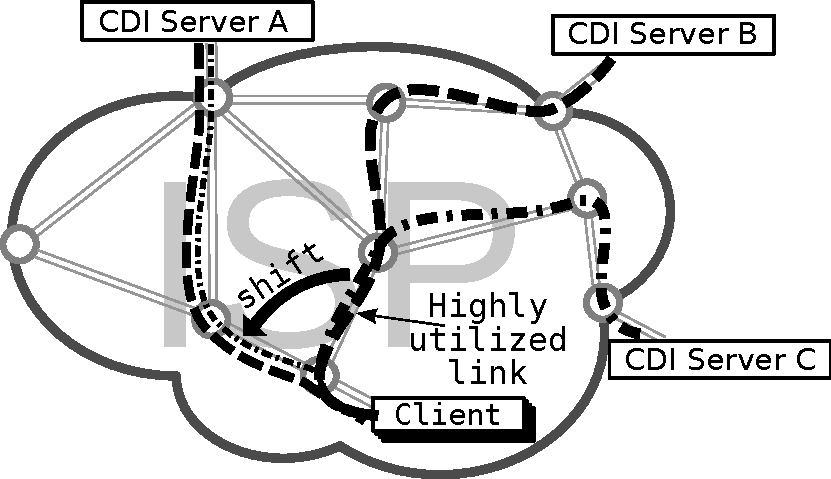
\includegraphics[width=0.90\linewidth]{figures-pdf/trafficShift-illustration}
\caption{Content-aware Traffic Engineering Process. Reprinted from \cite{Cate-CCR}. Included here by permission.}
\label{fig:Content-aware-illustration2}
\vspace{-1.5em}
\end{figure}


%%%%%%%%%%%%%%%%%%%%%%%%%%%%%%%%%%%%%%%%%%%%%%%%%%%%%%%%%%%%%%%%%%%%%%%%
\smallskip
\noindent {\bf Terminology:}\label{sec:Terminology}
%%%%%%%%%%%%%%%%%%%%%%%%%%%%%%%%%%%%%%%%%%%%%%%%%%%%%%%%%%%%%%%%%%%%%%%%
We denote as {\it flow} an OD flow between two routers in the network.  We call
a flow {\it splittable} if arbitrarily small pieces of the flow can be assigned
to other flows.  This is not to be confused with end-to-end sessions, \ie TCP
connections, which are \emph{un-splittable}.  The assumption that flows are
splittable is reasonable, as the percentage of traffic of a single end-to-end
session is small compared to that of a flow between routers. Let $C$ be the set
of nominal capacities of the links in the network $G$. We denote as {\it link
utilization} the fraction of the link capacity that is used by flows. We denote
as {\it flow utilization} the maximum link utilization among all links that a
flow traverses. We introduce the terms of {\it traffic consumer} and {\it
traffic producer} which refer to the aggregated demand of users attached to a
router, and the CDIs that are responsible for the traffic respectively. We
refer to the different alternatives from which content can be supplied by a
given CDI as \emph{network locations} that host servers.


%%%%%%%%%%%%%%%%%%%%%%%%%%%%%%%%%%%%%%%%%%%%%%%%%%%%%%%%%%%%%%%%%%%%%%%%
\ \\\noindent\textbf{Definition of CaTE:}\label{sec:CaTE-Definitions}\\\noindent
%%%%%%%%%%%%%%%%%%%%%%%%%%%%%%%%%%%%%%%%%%%%%%%%%%%%%%%%%%%%%%%%%%%%%%%%
We revisit traffic engineering by focusing on the traffic demands rather than
changing the routing.

\noindent \textbf{Definition 1: Content-aware Traffic Engineering(\cate)} is
the process of adjusting the traffic demand vector {\bf x}, given a routing
matrix $A$, so as to change the link traffic {\bf y}.

Not all the traffic can be adjusted arbitrarily. Only traffic for which
location diversity is available can be adjusted by \cate.  Therefore, {\bf
  x}={\bf x$_r$}+{\bf x$_s$} where {\bf x$_r$} denotes the content demands that
can be adjusted and {\bf x$_s$} denotes the content demands that can not be
adjusted as there is only a single location in the network where the content
can be downloaded from.  The amount of traffic that can be adjusted depends on
the diversity of locations from which the content can be obtained.  We can
rewrite the relation between traffic counts on links and traffic counts in
flows as follows: {\bf y}=$A$({\bf x$_s$} $+$ {\bf x$_r$}).  \cate adjusts the
traffic on each link of the network by adjusting the content demands {\bf
  x$_r$}: {\bf y$_r$}=$A${\bf x$_r$}. Applying \cate means adjusting the
content demand to satisfy a traffic engineering goal.


\noindent \textbf{Definition 2: Optimal Traffic Matrix} is the new traffic
matrix, {\bf x}$^*$, after applying \cate, given a network topology $G$, a
routing matrix $A$ and an initial traffic matrix {\bf x}.

Figure~\ref{fig:Content-aware-illustration2} illustrates the \cate process.  A
content consumer requests content that three different servers can deliver. Let
us assume that, without \cate, the CDI redirects the clients to servers B and
C.  Unfortunately, the resulting traffic crosses a highly-utilized link. With
\cate, content can also be downloaded from server A, thus, the traffic within
the network is better balanced as the highly utilized link is circumvented.

Minimizing the maximum utilization across all links in a network is a popular
traffic engineering goal~\cite{FT00,FT01,ImprovingPerformanceInternet2009}.  It
potentially improves the quality of experience and postpones the need for
capacity increase. \cate mitigates bottlenecks and minimizes the maximum link
utilization by re-assigning parts of the traffic traversing heavily loaded
paths. Thus it redirects traffic to other, less utilized paths.  Later in this
chapter, we will elaborate in Section~\ref{sec:impact}, different metrics such
as path length or network delay can also be used in \cate.


%%%%%%%%%%%%%%%%%%%%%%%%%%%%%%%%%%%%%%%%%%%%%%%%%%%%%%%%%%%%%%%%%%%%%%%%%
\ \\\noindent\textbf{CaTE and Traditional TE:}\label{sec:CaTE-TE}\\\noindent
%%%%%%%%%%%%%%%%%%%%%%%%%%%%%%%%%%%%%%%%%%%%%%%%%%%%%%%%%%%%%%%%%%%%%%%%%
\cate is complementary to routing-based traffic engineering as it does not
modify the routing. Routing-based traffic engineering adjusts routing weights
to adapt to traffic matrix changes. To avoid micro-loops during IGP
convergence~\cite{transient-IGP}, it is common practice to only adjust a small
number of routing weights~\cite{FT01}. To limit the number of changes in
routing weights, routing-based traffic engineering relies on traffic matrices
computed over long time periods and offline estimation of the routing weights.
Therefore, routing-based traffic engineering operates on time scales of hours,
which can be too slow to react to rapid change of traffic demands.  \cate
complements routing-based traffic engineering and can influence flows at
shorter time scales by assigning clients to servers on a per request
basis. Thus, \cate influences the traffic within a network online in a
fine-grained fashion.


%%%%%%%%%%%%%%%%%%%%%%%%%%%%%%%%%%%%%%%%%%%%%%%%%%%%%%%%%%%%%%%%%%%%%%%%
\ \\\noindent\textbf{CaTE and Multipath Routing:}\label{sec:CaTE-Multipath}\\\noindent
%%%%%%%%%%%%%%%%%%%%%%%%%%%%%%%%%%%%%%%%%%%%%%%%%%%%%%%%%%%%%%%%%%%%%%%%
Multipath routing helps end-hosts to increase and control their upload
capacity~\cite{PathSelection:CACM2011}. It can be used to minimize transit
costs~\cite{Optimizing:Goldenberg2004}. Multipath also enables ASes to
dynamically distribute the load inside networks in the presence of volatile and
hard to predict traffic demand
changes~\cite{TrafficDemand:ToN2001,MATE2001,TeXCP,Replex}.  This is a
significant advantage, as routing-based traffic engineering can be too slow to
react to phenomena such as flash crowds. Multipath takes advantage of the
diversity of paths to better distribute traffic.

\cate also leverages the path diversity, and can be advantageously combined
with multipath to further improve traffic engineering and end-user
performance. One of the advantages of \cate is its limited investments in
hardware deployed within an ISP. It can be realized with no change to routers,
contrary to some of the previous multipath
proposals~\cite{TeXCP,MATE2001,Replex}.  The overhead of \cate is also limited
as no state about individual TCP connections needs to be maintained, contrary
to multipath~\cite{TeXCP,MATE2001,Replex}.  In contrast
to~\cite{MATE2001,TeXCP}, \cate is not restricted to MPLS-like solutions and is
easily deployable in today's networks.


%%%%%%%%%%%%%%%%%%%%%%%%%%%%%%%%%%%%%%%%%%%%%%%%%%%%%%%%%%%%%%%%%%%%%%%%
\ \\\noindent\textbf{CaTE and Oscillations:}\label{sec:CaTE-Oscilations}\\\noindent
%%%%%%%%%%%%%%%%%%%%%%%%%%%%%%%%%%%%%%%%%%%%%%%%%%%%%%%%%%%%%%%%%%%%%%%%
Theoretical results~\cite{AdaptiveRouting2005,Convergence:Fischer2006} have shown that
load balancing algorithms can take advantage of multipath while provably avoiding traffic
oscillations. In addition, their convergence is fast. Building on these theoretical results, Fischer
et al. proposed REPLEX~\cite{Replex}, a dynamic traffic engineering algorithm that exploits
the fact that there are multiple paths to a destination. It dynamically changes the traffic load
routed on each path. Extensive simulations show that REPLEX leads to fast convergence, without
oscillations, even when there is lag between consecutive updates about the state of the network.
\cate is derived from the same principles and thus inherits all the above-mentioned desired properties.



%%%%%%%%%%%%%%%%%%%%%%%%%%%%%%%%%%%%%%%%%%%%
\subsubsection{Potential of Collaboration}\label{sec:impact}
%%%%%%%%%%%%%%%%%%%%%%%%%%%%%%%%%%%%%%%%%%%%

In this section, we quantify the potential benefits of \cate when deployed
within an European Tier-1 ISP using operational data.

%%%%%%%%%%%%%%%%%%%%%%%%%%%%%%%%%%%%%%%%%%%%%%%%%%%%%%%%
\noindent\textbf{Experimental Setting:}\label{sec:Experimental-Setting}
%%%%%%%%%%%%%%%%%%%%%%%%%%%%%%%%%%%%%%%%%%%%%%%%%%%%%%%
To evaluate \cate, an understanding of the studied ISP network is necessary,
including its topological properties and their implications on the flow of
traffic.  Indeed, the topological properties of the ISP network influence the
availability of disjoint paths, which are key to benefit from the
load-balancing ability of \cate.  Because \cate influences traffic aggregates
inside the ISP network at the granularity of requests directed to CDIs,
fine-grained traffic statistics are necessary.  Traffic counts per-OD flow,
often used in the literature, are too coarse an input for \cate.

%%%%%%%%%%%%%%%%%%%%%%%%%%%%%%%%%%%%%%%%%%%%%%%%%%%%%%%%
\noindent\textbf{Data from a Large European ISP:}\label{sec:Residential-Traces}
%%%%%%%%%%%%%%%%%%%%%%%%%%%%%%%%%%%%%%%%%%%%%%%%%%%%%%%
To build fine-grained traffic demands, we rely on anonymized packet-level
traces of residential DSL connections from a large European Tier-1 ISP,
henceforth called \emph{ISP1}. For ISP1, we have the complete annotated
router-level topology including the router locations as well as all public and
private peerings. ISP1 contains more than $650$ routers and $30$ peering points
all over the world.  Using the same monitoring infrastructure as in
Section~\ref{sec:traces}, we collect a $10$ days long trace of HTTP and DNS
traffic starting on May 7, 2010. We observe 720 million DNS messages as well as
more than 1 billion HTTP requests involving about 1.4 million unique hostnames,
representing more than 35 TBytes of data. We note that more than 65\% of the
traffic volume is due to HTTP.

A large fraction of the traffic in the Internet is due to large CDIs, including
CDNs, hyper-giants, and OCHs, as reported in earlier
studies~\cite{TrafficTypesGrowth:2011,arbor,PADIS2010}. In
Figure~\ref{fig:CDF-Traffic-CPs}, we plot the cumulative fraction of HTTP
traffic volume as a function of the CDIs that originate the traffic. For this,
we regard a CDI as a organizational unit where all servers from the distributed
infrastructure serve the same content, such as Akamai or Google.  We rank the
CDIs by decreasing traffic volume observed in our trace. Note that the x-axis
uses a logarithmic scale. The top 10 CDIs are responsible for around 40\% of
the HTTP traffic volume and the top 100 CDIs for close to 70\% of the HTTP
traffic volume. The marginal increase of traffic is diminishing when increasing
the number of CDIs. This shows that collaborating directly with a small number
of large CDIs, can yield significant savings.

In Figure~\ref{fig:CPs-Total-Traffic} we plot the traffic of the top 1, 10, 100
CDIs by volume as well as the total traffic over time normalized to the peak
traffic in our dataset.  For illustrative purposes, we show the evolution
across the first $60$ hours of our trace. A strong diurnal pattern of traffic
activity is observed. We again observe that a small number of CDIs are
responsible for about half of the traffic. Similar observations are made for
the rest of the trace.

\begin{figure}[tbp]
\center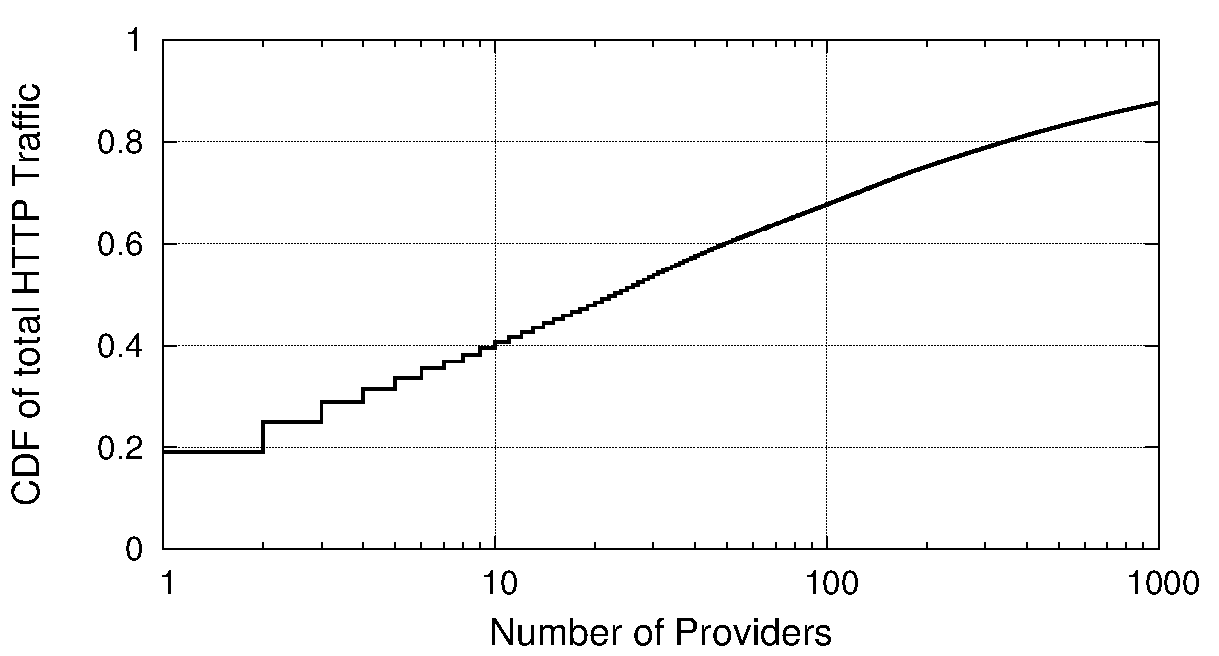
\includegraphics[width=1\linewidth]{figures-pdf/providersVsVolume}
\caption{CDF of traffic volume of CDIs in ISP1. Reprinted from \cite{Cate-CCR}. Included here by permission.}
\label{fig:CDF-Traffic-CPs}
\vspace{-1.5em}
\end{figure}


\begin{figure}[tbp]
\center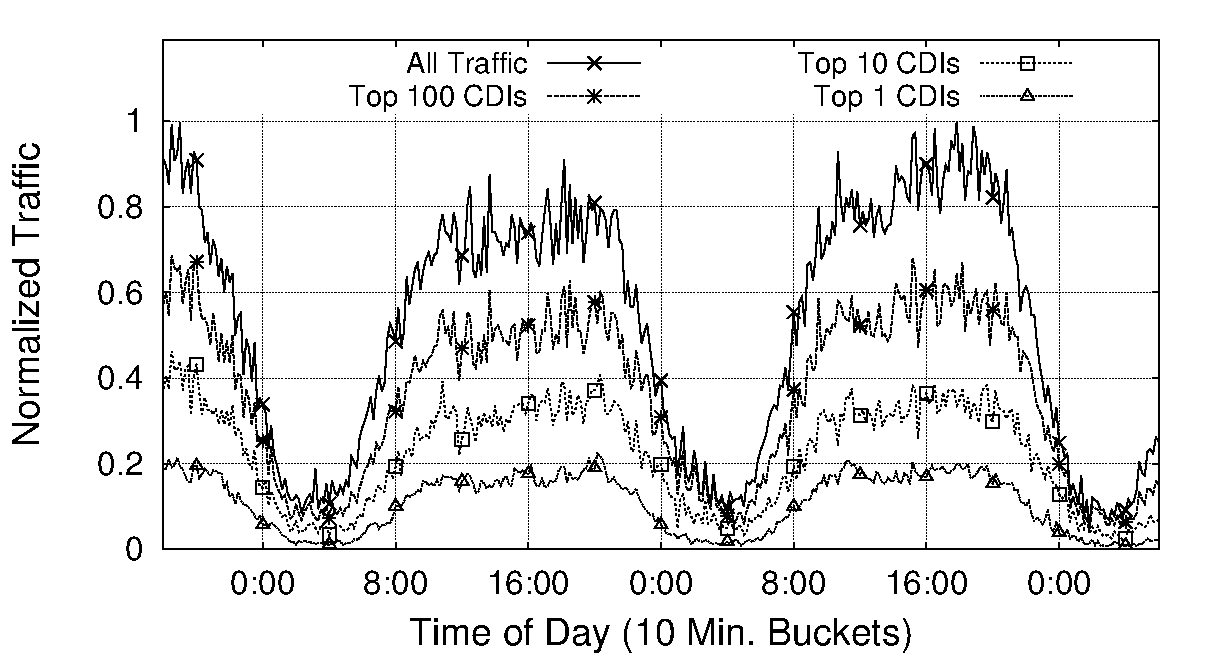
\includegraphics[width=1\linewidth]{figures-pdf/Volume_timeseries}
\caption{Normalized traffic for top CDIs by volume in ISP1. Reprinted from \cite{Cate-CCR}. Included here by permission.}
\label{fig:CPs-Total-Traffic}
\vspace{-1.5em}
\end{figure}



%%%%%%%%%%%%%%%%%%%%%%%%%%%%%%%%%%%%%%%%%%%%%%%%%%%%%%%%%%%%%%%%%%%%%%%%%%%%%%%%%%%
\noindent\textbf{Understanding the Location Diversity of CDIs:}\label{sec:Traffic-by-Content-Provider}
%%%%%%%%%%%%%%%%%%%%%%%%%%%%%%%%%%%%%%%%%%%%%%%%%%%%%%%%%%%%%%%%%%%%%%%%%%%%%%%%%%%
To achieve traffic engineering goals, it is crucial to also understand the
location diversity of the top CDIs, as \cate relies on the fact that the same
content is available at multiple locations.  Traffic originated from multiple
network locations by a given CDI is seen by \cate as a single atomic traffic
aggregate to be engineered. Furthermore, as routing in the Internet works per
prefix, we assume that the granularity of subnets is the finest at which \cate
should engineer the traffic demand. Thus, we differentiate candidate locations
of CDIs by their subnets and quantify the location diversity of CDIs through the
number of subnets from which content can be obtained.

We examine the amount of location diversity offered by CDIs based on traces from
ISP1.  To identify the subnets of individual CDIs, we rely on a similar
methodology to the one from Poese \etal~\cite{PADIS2010}. Our granularity is
comparable to their "infrastructure redirection
aggregation". Figure~\ref{fig:VolumeChoices} shows the cumulative fraction of
HTTP traffic as a function of the number of subnets (logarithmic scale) from
which a given content can be obtained, over the entire $10$ days of the
trace. We observe that more than $50\%$ of the HTTP traffic can be delivered
from at least $8$ different subnets, and more than $60\%$ of the HTTP traffic
from more than $3$ locations. These results confirm the observations made
in~\cite{PADIS2010}.


\begin{figure}[tbp]
\center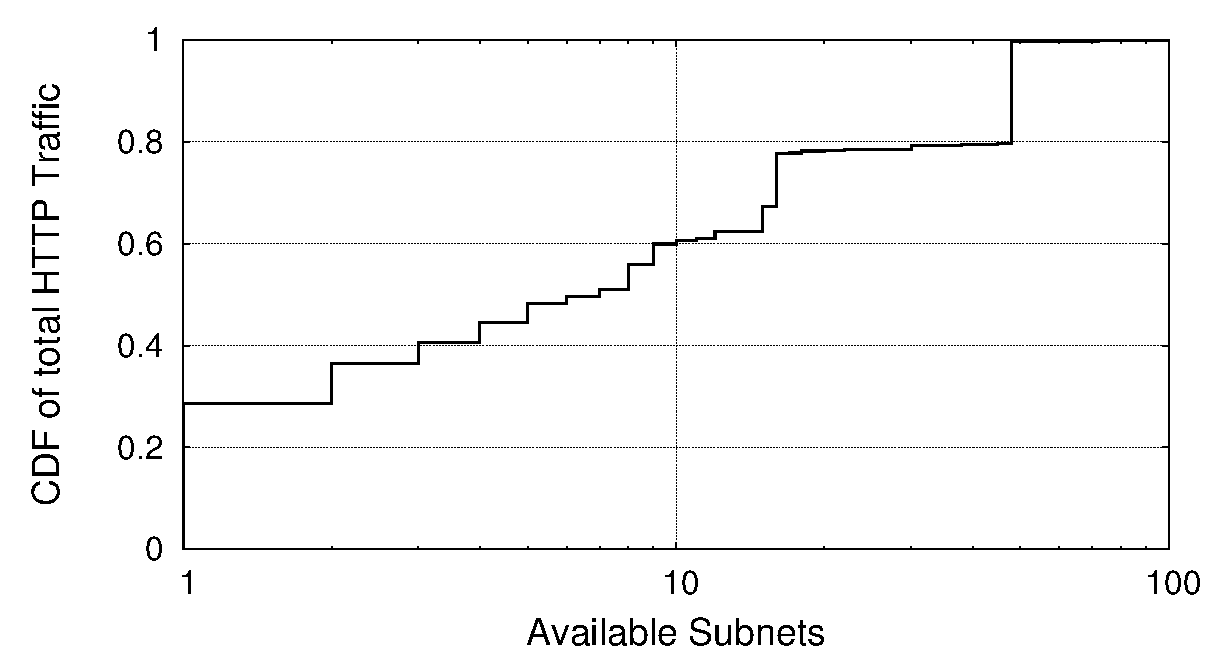
\includegraphics[width=1\linewidth]{figures-pdf/subnetVsVolumeBucket}
\caption{Subnet diversity from which content is available.}
\label{fig:VolumeChoices}
\vspace{-1.5em}
\end{figure}



%%%%%%%%%%%%%%%%%%%%%%%%%%%%%%%%%%%%%%%%%%%%%%%%%%%%%%%%%%%%%%
\noindent\textbf{Dynamics in Location Diversity:}\label{sec:Server-Dynamics}
%%%%%%%%%%%%%%%%%%%%%%%%%%%%%%%%%%%%%%%%%%%%%%%%%%%%%%%%%%%%%%
So far the location diversity of CDIs has been evaluated irrespective of time.
To complement the finding, we turn our attention to the location diversity
exposed by CDIs at small time-scales, \ie in the order of minutes.  To this
end, we split the original trace into $10$ minutes bins.
Figure~\ref{fig:TemporalEffect} shows the evolution of the number of exposed
subnets of five of the top 10 CDIs by volume.  Note that the diversity exposed
by some CDIs exhibits explicit time of day patterns, while others do not. This
can be due to the structural setup or the type of content served by the CDI.
The exposed location diversity patterns, \ie flat or diurnal, are
representative for all CDIs with a major traffic share in our trace. We
conclude that a significant location diversity is exposed by popular CDIs at
any point in time, and is quite extensive during the peak hour.

\begin{figure}[tbp]
\center
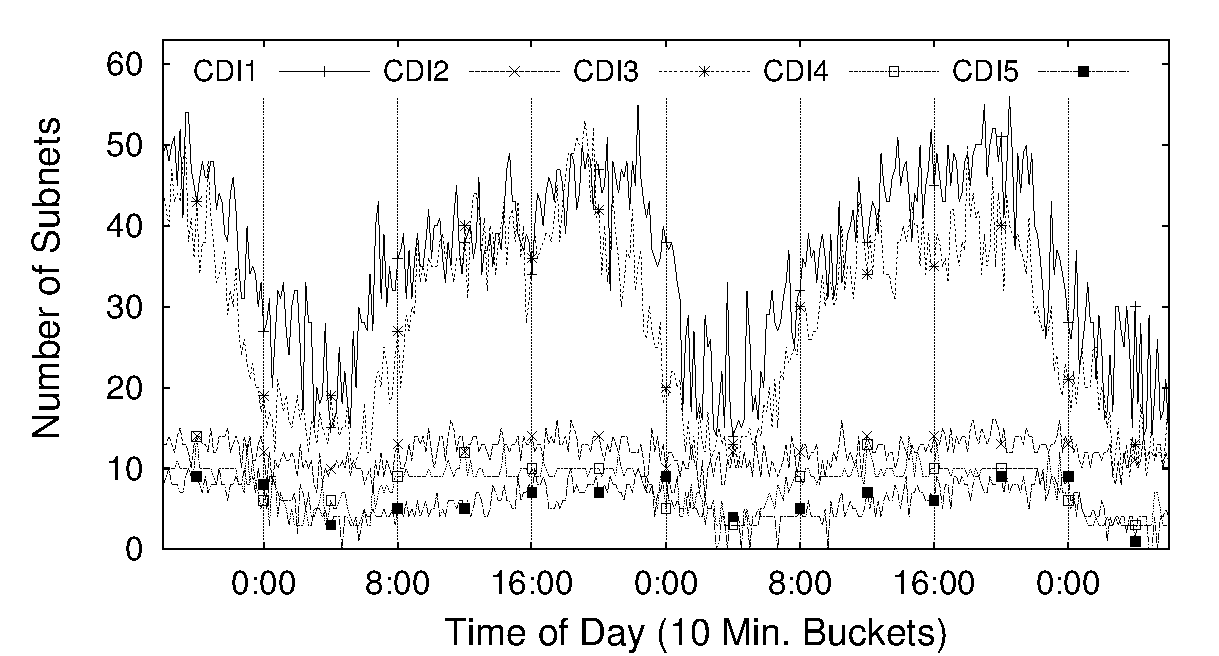
\includegraphics[width=1\linewidth]{figures-pdf/SubnetChoice_r-2}
\caption{Evolution over time of number of subnets for selected CDIs in
  the top 10 CDIs. Reprinted from \cite{Cate-CCR}. Included here by permission.}
\label{fig:TemporalEffect}
\vspace{-1.5em}
\end{figure}



%%%%%%%%%%%%%%%%%%%%%%%%%%%%%%%%%%%%%%%%%%%%%%
\noindent\textbf{Content Demand Generation:}\label{sec:TM}
%%%%%%%%%%%%%%%%%%%%%%%%%%%%%%%%%%%%%%
The location diversity is not a mere observation about CDIs deployment. It
requires to revisit the mapping between a given content demand and the realized
traffic matrix. Given the location diversity for content, multiple traffic
matrices can be realized from a given content demand. The standard view of the
OD flows therefore provides an incomplete picture of the options available for
\cate.

As an input for \cate, we introduce an abstraction of the demand that reflects
the available location diversity.  We rely on the notion of \emph{potential
  vectors}, that were denoted as $x_{r}$ in Section~\ref{sec:CaTE-Definitions}.
To generate the potential vector for a given CDI, the amount of traffic this CDI
originates as well as the potential ingress points need to be known. Combining
all potential vectors and $x_{s}$, we synthesize a network-wide content demand
matrix for each time bin, by scaling the traffic demand to match the network
utilization of ISP1.  For our evaluation, we use the series of content demand
matrices over a period of $10$ days. The content demands are based exclusively
on the HTTP traffic of our trace.


\subsection{Summary}

In this section we presented the potential of the \emph{Oracle} and
\emph{Content-aware Traffic Engineering} (\cate), two collaborative approach to
improve content delivery while achieving traffic engineering goals.  Both
leverage location diversity offered by P2P systems or CDIs. Moreover, \cate
enables dynamic adaption to traffic demand shifts. With \cate/the oracle the
decision on end-user to server/peer assignment can be done jointly between the
CDI/P2P system and the ISP.  Our analysis of operational data from a European
Tier-1 ISP has shown ample opportunities for \cate to improve content delivery
as it is done today.

Through extensive experiments, we show that both P2P users and ISPs benefit
from ISP-aided P2P locality, measured in terms of improved content download
times, increased network locality of query responses and desired content, and
overall reduction in P2P traffic. For a more detailed analysis of the possible
improvements and additional background information on the parameter set and
resulting improvements, we refer the reader to~\cite{afs-cispp2pcip-ccr07,A-IANSPS-08}.

In~\cite{Cate-CCR, CaTE-TR, Sigmetrics2012} we quantify the benefits of \cate
and consider one of the most popular traffic engineering goals, namely
minimizing the maximum utilization of the links in the
network~\cite{FT00,FT01}.  Our evaluation shows that \cate yields encouraging
results, even when only a few large CDIs are collaborating with an ISP. In fact,
even metrics that are not directly related to the optimization function of
\cate are improved. Besides significant improvements for the operation of ISP
networks, the end-users to also benefit from these gains. This can be
attributed to the decrease of delay as well as the reduced link
utilization. In~\cite{CaTE-TR} we also consider other network metrics such as
path length or path delay and the effect of other network topologies.  We also
outline how \cate can aid in the deployment of popular large scale
applications, \eg NetFlix, by selecting strategic locations for caches and
specific optimization goals to support their operation. With this we conclude
the section on collaborative traffic engineering and continue to elaborate on
our idea for ``in-network server deployment'' in the next chapter.


%
%\newpage
%%%%%%%%%%%%%%%%%%%%%%%%%%%%%%%%%%%%%%%%%%%%
\section{Future of Collaboration}\label{sec:future}
%%%%%%%%%%%%%%%%%%%%%%%%%%%%%%%%%%%%%%%%%%%%


\padis and \cate are designed to enable cooperation between CDI and ISPs for
the already deployed servers. Recent advances in virtualization offer CDIs
additional degree of freedom to scale-up or shrink the footprint on demand.
This can be done either by jointly deploying and operating new servers with the
ISPs.  In this section we formally introduce the design of on-demand services
motivated by the recent announcement of major ISPs to support generic
hardware-network appliances, also referred to as microdatacenters, and offer
them to application, service, and content providers. We also provide the design
and implementation of \Netpaas, a system to orchestrate the deployment of
on-demand services inside microdatacenters, by utilizing the view of the ISP
about the network and additional computation and storage resources inside the
network.

\subsection{The New Cloud: Microdatacenters Deep Inside the Network}\label{sec:generic-appliances}

Applications are increasingly relying on direct interactions with end-users and
are very sensitive to delay~\cite{ImprovingPerformanceInternet2009}. Indeed,
transaction delay is critical for online
businesses~\cite{amazon-study-about-transaction-speed}.  Network delay and loss
are important contributors.  Today, large-scale service deployments are
restricted by limited locations in the network, \eg datacenters, peering
locations, or IXPs. These locations are not necessarily ideal~\cite{CloudCmp}.
We point out that \emph{selection of service location is critical and currently
not flexible enough}.  Services should be located close enough to, in terms of
network distance, the clients.  Since client demands are volatile and change
across time, CDIs need agility~\cite{EmbrassingleDistributed}.  They can
improve their service quality by quickly allocating, de-allocating, and
migrating resources on-demand where and when they are needed. Indeed, since
delay and packet loss are among the critical metrics, the service may need to
be deployed deep inside the network, as many ISPs do for IPTV services. This
option is not yet available for non-ISP content delivery Infrastructures, \eg
for cloud services.

Currently, most services and networks are run by independent entities with
different and often conflicting objectives. Lack of information about the other
entity leads to suboptimal performance and resource allocation for both the CDI
and the ISP. For example, CDIs implement sophisticated methods to infer network
conditions to improve perceived end-user experience~\cite{Akamai-Network}, \eg
active measurements within the ISPs. Yet, the information gleaned from these
measurements is already available with far greater precision to the ISP. On the
other hand, ISPs continuously upgrade their infrastructures without being able
to efficiently engineer the CDI traffic flows~\cite{PADIS2010}. Today,
cooperation and/or partnership between providers is limited to, \eg peering or
lately direct interconnections with content delivery Infrastructures. This
level of cooperation is too narrow to reduce operational costs, improve
end-user experience, circumvent bottlenecks, handle flash crowds, and adapt to
changing network conditions and user demands. This has led to initial
discussions on how to improve communication between the various entities, \eg
within the IETF ALTO and CDNi working groups.


\subsubsection{The ISPs Proposal}\label{NFV}

To overcome the above mentioned obstacles in service deployment and operation,
major ISPs, including AT\&T, Verizon, Deutsche Telekom, Telefonica, NTT, have proposed
the use of cloud resources consisting of general purpose appliances that are
co-located at network aggregation points inside the ISP. With the convergence
of computing, storage, and communications, the acceptance of cloud services,
and the ever increasing demand for popular services, ISPs are moving towards
deploying general-purpose computing and storage infrastructures in their points
of presences (PoPs). Henceforth, we refer to these as \emph{microdatacenters}.
The description of the functionality of these microdatacenters is provided in a
white paper~\cite{NFV} that appeared in the SDN and OpenFlow World Congress in
October 2012 and signed by 13 of the largest ISPs. Microdatacenters can be also
the technical solution needed to materialize recent alliances of major CDIs,
such as Akamai with large ISPs in the area of content
delivery~\cite{content-delivery-alliance1,content-delivery-alliance2,content-delivery-alliance3}.
We notice that Software Defined Networks (SDNs) is another alternative to
redirect traffic or perform traffic engineering when applied within an ISP or
between and ISP and a CDN in cooperation.  The comparison of the two
approaches, NFV and SND, is out of the scope of this chapter and we refer the
users to the related literature on SDN
\eg~\cite{Ethane,NOX,OpenFlow,SDN-Internet-Infrastructure,B4}.

\begin{figure} 
\begin{center}
	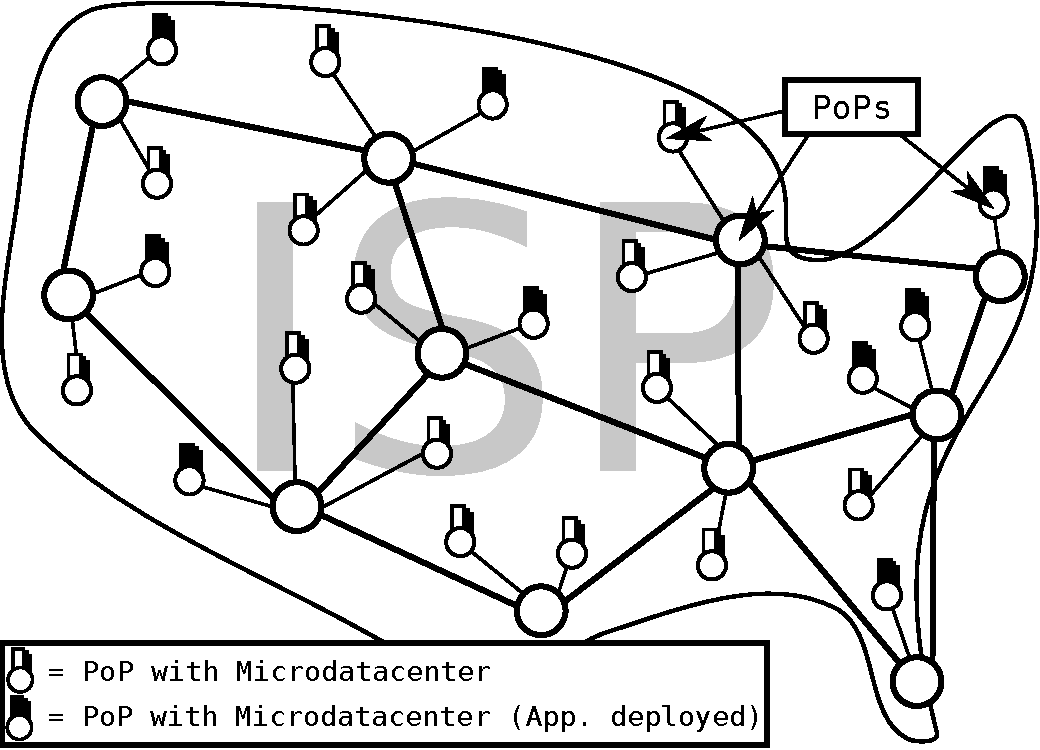
\includegraphics[width=0.9\linewidth]{figures-pdf/ISP+Content} 
\end{center}
\caption{\MDCs in an ISP with \Netpaas enabled} 
\label{fig:story} 
\end{figure}

Figure~\ref{fig:story} illustrates the basic idea. The ISP can offer
\emph{slices} within its microdatacenters, that can be leased by the
CDIs---using our proposed mechanism---based on their needs. This approach
leverages recent advances in virtualization technology, and flexible billing
models, such as pay-as-you-go, to provide cost-efficient and scalable service
deployment, enabling unprecedented flexibility.  Moreover, the diversity of
available service locations within the network can be used to improve end-user
experience and makes it possible to launch even more demanding applications,
such as interactive ones. On-demand service enables CDIs to rely on a fixed
infrastructure deployment for their baseline operation and then scale it up by
dynamically allocating resources closer to end-users. It also lowers the burden
of entrance in the service market for smaller CDIs who might rely exclusively
on the \onservice at first.

\subsubsection{Microdatacenter
Specifications}\label{sec:microdatacenters-specification}

Microdatacenters consist of one or more racks of off-the-shelf hardware
deployed in general purpose rack space at network aggregation points.
State-of-the-art solutions have been proposed by the VMware/Cisco/EMC VCE
consortium \cite{VCE}, and are also offered by other vendors, such as NetApp
and Dell.  These solutions are general-purpose and provide a shared
infrastructure for a large range of applications. They typically consist of two
basic components: hardware and management software.

\begin{description*} \item [Hardware:] Typical microdatacenters include
\emph{storage}, \emph{computing}, \emph{memory}, and \emph{network access}
components.  Storage consists of tens of Terabytes with an ultra-fast
controller providing I/O throughput in the order of hundreds of Gbps. The
storage component is connected to the Internet through multi-Gbps interfaces
and to the computing component with Gigabit Ethernet switches.  Typically, a
rack includes up to 40 physical multi-core blade servers as well as two routers
and two switches in mesh configuration, for redundancy and load balancing.
\item [Management Software:] Each vendor offers a set of management tools not
only for administering the components but also to create resource slices and to
delegate the operation of the slices to external entities. This can be done
per-server or via hardware supported virtualization\footnote{ For example,
para-virtualization~\cite{virtualization} presents the VM with an abstraction
that is similar but not identical to the underlying hardware.}. The management
software is also responsible for storage allocation and handling network
resources, including IP address space. In addition, the management tools come
with a monitoring interface that allows the ISP to monitor the utilization of
the overall microdatacenter as well as the information for each slice that can
be shared with the external entity.  \end{description*}

An ISP can allocate resource slices consisting of computing, storage, memory,
and network access in a microdatacenter and then delegate the operation of the
slice to a CDI. This is what we refer to as the \emph{ISPs cloud service} which
is realized via resource slices in microdatacenters throughout the ISPs
infrastructure.

\subsubsection{Microdatacenter Network Footprint}\label{sec:microdatacenters-footptint}

Most ISPs' networks consist of an access network to provide Internet access to
DSL and/or cable customers, as well as an aggregation network for business
and/or VPN customers. Routers at this level are often referred to as {\em edge
routers}.  The access and aggregation networks are then connected to the ISP's
backbone which consists of {\em core routers}.  {\it Border routers} are core
routers that are used to connect either to other networks or to co-location
centers.  Opportunities to deploy microdatacenters exist at each level: edge,
core, or border router locations.

The advantage of deploying service infrastructure only at the core router
locations is that there are a few large and well established locations. This is
also a disadvantage as location diversity might be limited. Location diversity
is highest at the edge router locations.  However, it might not always be
possible to deploy a microdatacenter, i.e., due to limited space and/or power
at the facilities, or due to cost. These locations, however, minimize the
distance to the customers.  Border router locations are often a subset of core
routers, hence they inherit the same advantages and disadvantages.

The advantage of using an ISP cloud service vs.\ a public cloud
service for a CDI is the chance to minimize the distance to the
end-user. \ondemandbase allows the CDI to control the
location of the slices and ensures that there are no major network
bottlenecks.


\subsection{\OnService Design}\label{sec:service-design}

An {\it \onservice} is a service of the ISP (see Figure~\ref{fig:story}) that
enables CDIs to use a hosting infrastructure that scales according to end-user
demands, so as to minimize its capital expenditures and operating costs, as
well as the distance between its hosting infrastructure and the source of the
demand.  Moreover, it offers an interface that enables the CDI to map user
requests to appropriate slices in order to maximize slice utilization and
minimize the distance between the end-user and the slices.

{\bf Definition 1: ISP \OnService.}  The ISP \onservice is a service offered by
the ISP and uses as its base unit of resource allocation the notion of a
microdatacenter \emph{slice}.  It is the ISP's task to allocate/de-allocate the
slices since it operates the microdatacenter.  The CDI requests slices based on
its clients demand. When the slice is allocated to the CDI, the service can be
installed on the slice. From that point on, the CDI fully controls the
operation of the service installed in the microdatacenter. Negotiation about
slices are done via the \emph{\onservice interface} through which CDI demands
are matched to the ISPs resources. How to map demands to resources in an
efficient manner is the task of the ISP and part of the \emph{\onservice
realization}.  In addition, the interface allows for access to the billing
information.  Moreover, the \emph{\onservice interface} enables the mapping of
user requests to appropriate slices.

The above mentioned use of microdatacenters is in-line with the available
primitives of private and public clouds operated in large-scale datacenters,
\eg~\cite{amazon,azure}.


\subsubsection{Microdatacenter Slice}\label{sec:Slice}

Based on our description of microdatacenters in the previous sections, we define
a slice as follows.

{\bf Definition 2: Slice.} The slice of a microdatacenter is a set of
physical or virtualized resources of a specific capacity, for each of the
resources of the microdatacenter. The slice is delegated to the service
provider that can install and operate its service using the resources of
the slice.

For example, a slice can be a 1-core server with 2 GB RAM, 30 GB storage, a
1 Gbps Internet access bandwidth, 2 public IPs---an actual physical resource.
Alternatively, it can be a VServer with 2GB and 1 Gbps Internet
access bandwidth, 1 public IP, and a pre-installed OS---a virtual machine
of a specific type.  With the current management and virtualization tools
available from microdatacenter vendors, it is possible to
allocate/deallocate slices on-demand in with unprecedented degree of
freedom, \eg~\cite{aboveclouds} and references within.


\subsubsection{\OnService Realization}\label{sec:Realization}

Based on the above specification of \onservice, the ISP has to implement two
functions to offer its \onserviceemph: \emph{mapping of service pro\-vi\-der
demands to slices} and \emph{assigning users to slices}.

Note, the time scales at which these two services are expected to be used
differ significantly. The first one allows the service provider to flexibly
allocate and de-allocate its slices based on its forecast of demands, in those
locations where it wants them.  We foresee that requests for slices are not
issued individually but rather collectively on a time scale of tens of minutes
or hours.

The CDI provides the ISP with a set of demands for slice resources, predicted
demand locations, desired slice locations, as well as optimization criteria.
The ISP then has to map the demands to its microdatacenter resources.  We
expect that the major degree of freedom that the ISP uses to jointly optimize
performance is the desired slice location. We refer to this optimization
problem as the \sliceallocation problem. If the desired slice locations are
fully specified or the predicted demand locations are missing, the
\sliceallocation problem becomes trivial and the ISP only grants or denies the
request.

At the second time scale, the ISP can help the CDI in assigning users to
slices. Since the service is offered at multiple locations, a good assignment
of users to slices impacts not only the load on the network but also the
network delay and packet loss, which are key contributors to the user
experience. Jointly optimizing this mapping is therefore of interest to both
the ISP and the CDI. The CDI can query the ISP for each request on where to map
it, based on the current set of slice assignments and service loads. The ISP
then uses its network information to propose possible slices. We refer to this
problem as the \sliceassignment problem, see \cite{Cate-CCR}.

Another degree of freedom \onservice offers to the CDI is auto-scaling.  While
it is quite feasible to dimension applications, flash-crowds or device failures
are hard to predict. To this end, a CDI may allow \onservice to create replicas
if its monitoring indicates that the capacity of the service at a given
location is or will be exceeded.  To realize this service, the ISP needs to
constantly monitor resource availability and if necessary migrate or suggest
the creation of additional slices. Moreover, it has to allow the CDI to monitor
the utilization of its slices.


\subsubsection{Service Interfaces}\label{sec:service-interfaces}

The ISP offers four interfaces to the content delivery Infrastructures:

\begin{description*}

\item [Resource discovery:] Using this interface the CDI requests information
about resources, e.g., about available locations for slices and if in principle
slices are available at those locations at what price.

\item [Slice allocation:] Using this interface the CDI requests slice
allocation within a certain cost limit.

\item [User-slice assignment:] Using this interface the CDI requests
recommendations for user demand to slice mapping.

\item [Monitoring and billing:] Using this interface the CDI monitors the
status and cost of its slices.

\end{description*}

In Section~\ref{sec:future-netpaas} we give specific examples of how these
service interfaces can be used by a CDI and ISP to cooperate in order to
improve their services.


\subsubsection{Billing}\label{sec:billing}

It is important for the CDI to minimize and track the cost of its use of
\onservice.  Depending on the scale of the services, the service provider has
to pay the usual price or negotiate bilateral agreements with the ISP. Using
the resource discovery interface, it estimates the cost of slice allocation at
possible locations. Using the slice allocation interface, it can bound the
total cost of the request.

We expect that the billing of a slice allocated via \onservice follows that of
large-scale datacenters.  This means that there is an installation cost and a
usage cost.  The installation cost applies to a single slice in a
microdatacenter and is charged only once or over long time intervals, \eg
hours, and is fixed. The installation cost typically increases if additional
licenses have to be leased, \eg software licenses. The installation cost can
depend on the location of the microdatacenter that hosts the slice or the
time-of-day.

The usage cost follows a pay-as-you-go billing model and charges for the usage
of different resources assigned to a slice.  The billing among different
resources in the same slice can be quite diverse. The slice can use expensive
resources such as bandwidth or cheaper ones such as CPU.

For example, a slice may have a $\$ 0.01$ per hour installation cost and a
usage cost that depends on its use of various resources, \eg $\$ 0.02$ per real
CPU usage per hour, $\$ 0.001$ per GByte stored per hour, and $\$ 0.001$ per
Gbps outgoing traffic per hour.  If the slice is idle, then only the
installation cost is charged. Note, that if the slice is used for a short
period within the allocation time, \eg a few minutes, then the charge may apply
to the minimum billing granularity.

To minimize the cost of deploying an on-demand service, the CDI can change its
total slice demands as well as its slice specifications dynamically. Moreover,
it can relax the slice specifications to reduce overall cost of its service
deployment.



\subsection{Network Platform as a Service (NetPaaS)}\label{sec:future-netpaas}

Next, we discuss the prototype system that has been proposed to materialize the
On-demand service, Network Platform as a Service (NetPaaS). NetPaaS leverages
the view of PaDIS and also utilize the knowledge about the status of the
microdatacenters within the network. NetPaaS is also able to map the requests
of CDIs to available microdatacenters to better match the demand with the
resources inside the network.  The granularity at which they are exchanged via
the service interface.  We also outline several possible protocols for the
service interfaces. We focus on resource discovery, slice allocation, and
user-slice assignment. We do not discuss monitoring and billing because they
can be realized today using techniques similar to those in use by current
public clouds, \eg~\cite{aboveclouds}. Due to space limitations, we refer the
reader to \cite{NetPaaS} for a formalization of NetPaaS, as well as an
evaluation on a CDI use case.

Recall that our assumption that the time scales at which the two principle
components of \onservice operate are different. On the one hand, resource
discovery and slice allocation are expected to be done on time scales of tens
of minutes, hours, or even days. On the other hand, user-slice assignment
potentially happens on a per user request basis. Accordingly, the protocols
differ. We propose to use out-of-band protocols for the first two service
interfaces and in-band protocols for the third one.


\subsubsection{Resource Discovery}\label{sec:Resource-Discovery}

The purpose of resource discovery is to provide the CDI with the ability to
gather information about the resources offered by the ISP. Accordingly, we
have two message types: CDI\_Discovery\_Request and ISP\_Discovery\_Re\-sponse.

\begin{description*}

\item [CDI\_Discovery\_Request:] Is issued either without and with arguments.
In the first case the response is the set of resources that are offered. In the
second case the responds contains details about the resources named in the
argument.

\item [ISP\_Discovery\_Response:] List of available resource or details about
the resources specified in the argument.

\end{description*}

So far we have not outlined at what granularity and specificity the resources
are requested. This depends on the agreements between the CDI and the ISP.  For
example, the ISP may have no problem revealing its microdatacenter locations to
a major CDI. However, it may not want to share this information with an
untrusted CDI that wants to run a single slice. For the latter, the region in
which the microdatacenter is located might well suffice.

With regards to granularity, the ISP can specify which type of servers it is
offering in each microdatacenter region, as is common for public cloud
services~\cite{amazon}, unless another agreement is in place that enables
access to more specific information.  With regards to the availability and/or
price, the ISP can either return a base price, including installation and usage
cost, to indicate that resources are available or offer an auction-based
system. In the latter case, the discovery request returns information about
past prices.

\subsubsection{Slice Allocation}\label{sec:system-slice-allocation}

\begin{figure}
    \begin{center}
    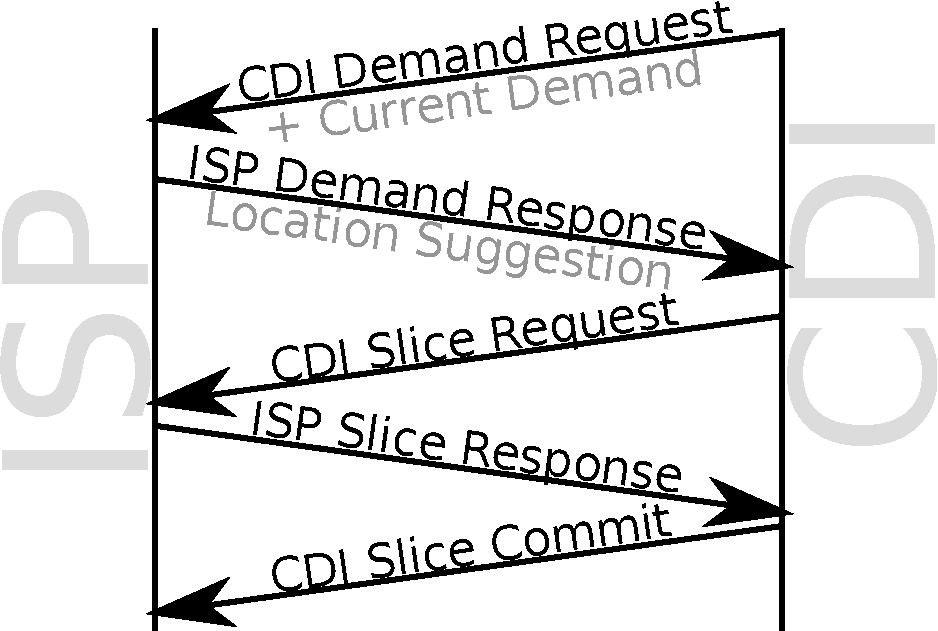
\includegraphics[width=0.6\linewidth]{figures-pdf/Resource_Negotiation}
    \end{center}
    \vspace*{-1em}
    \caption{Slice allocation message exchange.}
    \label{fig:ResourceAllocation}
\end{figure}

Slice allocation enables the CDI and ISP to cooperate for allocating slices in
microdatacenters close to the end-user that are able to satisfy the demands.
We envision five message types: CDI\_Demand\_Request, ISP\_Demand\_Response,
CDI\_ Slice\_Request, ISP\_Slice\_Response, CDI\_Slice\_Commit. The first two
message types enable the cooperation between the CDI and the ISP to allocate
slices at appropriate microdatacenter by utilizing network information, see
Figure~\ref{fig:ResourceAllocation}. The last three messages enable a three way
handshake between the CDI and the ISP to verify that the ISP is able to provide
a specific slice for the CDI.

\begin{description*}

\item [CDI\_Demand\_Request:] Is submitted by the CDI to the ISP and contains a
summary of the hardware resources the CDI wants together with optimization
criteria, constraints, and a demand forecast, \eg per region or per network
prefix.  Possible optimization criteria are to minimize network distance or the
cost. The constrains include: number of locations, minimum resources per slice,
etc.

\item [ISP\_Demand\_Response:] The ISP returns a set of proposed slice
configurations and their price. It computes these by solving the
\sliceallocation problem.

\item [CDI\_Slice\_Request:] The CDI either selects, based on its criteria, a
set of proposed slices as returned by the ISP\_De\-mand\_Response, or it
completes a specification of a slice set request using information it retrieved
via the resource discovery interface. In addition, the request contains a
maximum cost.

\item [ISP\_Slice\_Response:] Upon receiving a CDI\_Slice\_Request, the ISP
checks if it can offer the set of slices at the requested cost. This involves
solving another version of the \sliceallocation problem. If possible, the ISP
returns the price otherwise it declines the request.  At this step, the ISP
reserves the requested resources to guarantee their availability. Note, the ISP
does not have to return precise slice definitions, \eg instead of returning
that slice x should be located in microdatacenter~y attached to router~z it
only returns slice~x should be located in region~xyz.

\item [CDI\_Slice\_Commit:] This step confirms CDI\_Slice\_Requests. Upon
receiving the commit from the CDI, the ISP allocates the slices and delegates
their control to the CDI.  

\end{description*}

Now we discuss different ways in which a CDI and an ISP can cooperate using the
above messages. These ways differ in which information is shared and with whom.

\begin{description*}

\item [Minimum information exchange:] The CDI uses the information from the
ISP\_Demand\_Response for queries via CDI\_Demand\_Request with a uniform
distributed demand vector. The responses include slice candidates with servers
having specified hardware profiles and in specific regions. Then, the CDI
scales the suggested slices according to its demand locations and uses the
CDI\_Slice\_Request message to check if the ISP can offer it and at what price.
Once it has found a satisfactory configuration it can use the
CDI\_Slice\_Commit message to request the necessary slices.


\item [Partnership 1:] The CDI uses CDI\_Demand\_Request with a scaled demand
CDI selects one of these and uses the ISP\_Slice\_Request message so that the
ISP can reserve the resources. Upon successful reservation, the
CDI\_Slice\_Commit message confirms the allocation of the slices.

\item [Partnership 2:] The CDI uses the CDI\_Demand\_Request without a demand
vector but with specific resource requests. The ISP response specifies
candidate microdatacenters with available resources.  Then, the CDI uses its
version of the \sliceallocation problem to find possible slice sets at a subset
of these locations. Then, the CDI uses the ISP\_Slice\_Request message to see
if the ISP can offer it and at what price. Once it finds a satisfactory
configuration it uses the CDI\_Slice\_Commit message to allocate the slices.

\end{description*}

The first scenario corresponds to the minimum information that has to be
exchanged in order to reach a consensus on the locations and specification of
the slices. The latter two summarize different forms of possible cooperations
that can be agreed upon in bilateral agreements.

So far, we have assumed that there are no preallocated slices. However, this is
typically not the case, and the actual task is to augment a preexisting set of
slices in such a way as to best serve the predicted demand for the next time
period. To enable this, another argument to each message request can be
provided, indicating a set of already allocated resources and a penalty value
for deallocating slices in one location and allocating them in another.  This
penalty is needed as part of the optimization problem.  Basically, it indicates
up to which point it is preferable to keep a suboptimal location because of
stability of resource allocation vs.\ when to migrate the service to a new
location.  Based on the returned information, the CDI has the option of either
moving slices using VM migration or to de-allocate and allocate new slices.

The ISP microdatacenter can offer VM migration and/or
consolidation\footnote{Here, consolidation corresponds to moving multiple VMs
with minimal resource requirements to the same physical machine to keep a base
service.} with keeping the IP addresses only within the same microdatacenter
location. Across microdatacenters it may only offer migration with tunnels
which requires the CDI to temporarily operate two slices at both locations.
However, the old one is a good candidate for consolidation so that it is
possible to reduce the allocated resources to a minimum within a
microdatacenter once all new requests are served by the newly allocated slices.
Thus, if an ISP offers service consolidation, one option for CDIs that want to
use diverse sets of microdatacenters is to always keep a minimal slice active
at each location and expand or shrink it according to the demand.

\subsubsection{User-Slice Assignment}\label{sec:system-user-assignment}

\begin{figure}[tbp]
    \begin{center}
    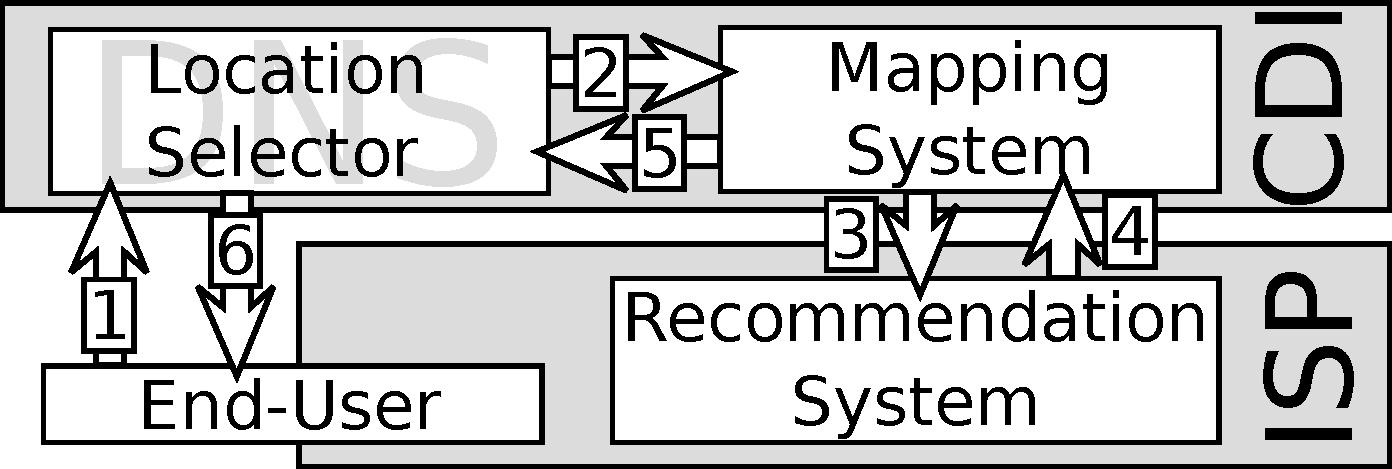
\includegraphics[width=0.8\linewidth]{figures-pdf/Mapping_System}
    \end{center}
    \vspace*{-1em}
    \caption{User-slice assignment schematic.}
    \label{fig:UserSliceAllocation}
\end{figure}

The purpose of the user-slice assignment interface is to enable small time
scale interactions between the CDI and the ISP, to ensure that end-user demand
is mapped to the appropriate slice.  Therefore, the interface has to be
integrated into the process used by the CDI to map user requests to CDI
servers.  Next, we first review how this is currently realized using DNS. Then,
we discuss options on how the user-slice assignment interface can be
integrated, see Figure~\ref{fig:UserSliceAllocation}.

{\bf CDI: User request to CDI server mapping.} Before an end-user issues a
request for the CDI service, \eg downloading some content or watching a video,
it issues a DNS request to map the hostname to an IP address of the server that
hosts the service.  This DNS request is sent to the ISPs DNS resolver or an
alternative DNS resolver. This resolver contacts the authoritative DNS server
of the CDI service, since caching is typically restricted by small TTL's. The
authoritative DNS server uses a CDI service, the CDI mapping system, to select
a CDI server from which to satisfy the future requests of this end-user. The
CDI mapping system performs a CDI specific optimization.  This optimization may
consider the load on the CDI servers, the network location of the CDI server as
well as the requesting DNS server, the price of network access at the CDI
server, etc. Note, the CDI's authoritative DNS name servers usually does not
have access to the IP address of the end-user as the request is forwarded via
the DNS resolver unless the eDNS~\cite{DNS-extension-IP-client} standard is
used.  With eDNS, the client IP address or the IP prefix can be added to the
DNS request sent by the DNS resolver to the authoritative DNS name server. In
addition, the CDI can use HTTP redirection to further load balance within its
infrastructure.


{\bf User-Slice Assignment: Option 1.} Considering the process outlined above,
one possible way to use the user-slice assignment interface is within the
optimization that the CDI mapping system performs.  For this case, we envision
two message types: CDI\_User-Slice\_Assign\_Re\-quest and
ICDI\_User-Slice\_Assign\_Response which correspond to steps 3 and 4 in
Figure~\ref{fig:UserSliceAllocation}.


\begin{description*}

\item [CDI\_User-Slice\_Assign\_Request:] Issued by the CDI's DNS server to the
  ISP. It contains the client IP address as well as slice locations within or
  outside of the ISP.

\item [ISP\_User-Slice\_Assign\_Response:] The ISP responses with a ranking of
  the slice locations.

\end{description*}

The previous two messages enable the CDI to consider information from the ISP,
conveyed via the ranking, for its mapping. This is equivalent to the
functionality and protocols proposed by the IETF ALTO working group.  However,
we envision a more light weight implementation. We propose to not rely on XML
for encoding each request if the granularity of the requests is on a per
connection level. If the CDI uses a coarser granularity such as subnet or
region, the efficiency of the message exchange is even less critical.\\

{\bf User-Slice Assignment: Option 2.}
Another way to integrate the user-slice assignment interface within
the above process is by pro-actively sharing information between the CDI
and the ISP.  For this case, we again envision two message types:
ISP\_User-Slice\_Assign\_Pro\-po\-sal and CDI\_User-Slice\_Assign\_Ack.

\begin{description*}

\item [ISP\_User-Slice\_Assign\_Proposal:] Is sent by the ISP to the CDI
  mapping system. It contains a set of IP prefixes each with an associated
  ranking of the different microdatacenter locations.

\item [CDI\_User-Slice\_Assign\_Ack:] The CDI either acknowledges or rejects
  the proposal.

\end{description*}

This again enables the CDI to include information from the ISP, conveyed via
the ranking, in its mapping.  For example, one can use BGP to send such
messages---a mechanism Akamai already utilizes to aid in mapping users to
its clusters~\cite{Akamai-Network}.


\subsection{Summary}

Motivated by the high requirements newly deployed services put on the ISPs
networks, we formally introduced the design of on-demand services to relieve
both the CDI and the ISP.  We also provided the design and implementation of
\Netpaas, a system to orchestrate the deployment of on-demand services using
the ISPs view of the network and available resources. In~\cite{NetPaaS} we
evaluate \Netpaas using operational traces from the biggest commercial CDN and
a European Tier-1 ISP. We quantify the benefits of \Netpaas by utilizing
different optimization goals \eg delay reduction or reduced link utilization.
Our results show that \Netpaas yields encouraging results for a joint
deployment of new services that significantly improves the end-users
performance while reducing the network utilization for the ISP and offering
agile service deployment to the CDI. For the analysis and performance evaluation of
on-demand server placement algorithms in wide-area networks we refer the reader
to~\cite{ToN-dFL} and \cite{SimultaneousSourceLocation}.


%
%\newpage
\section{Conclusion}\label{sec:conclusion}

People value the Internet for the content and the applications it makes
available~\cite{CCN}. For example, the demand for online entertainment and web
browsing has exceeded 70\% of the peak downstream traffic in the United
States~\cite{sandvine}. Recent traffic
studies~\cite{TrafficTypesGrowth:2011,arbor,PADIS2010} show that a large
fraction of Internet traffic is originated by a small number of Content
Distribution Infrastructures (CDIs). Major CDIs include highly popular
rich-media sites such as YouTube and Netflix, One-Click Hosters (OCHs), \eg
RapidShare, Content Delivery Networks (CDNs) such as Akamai, and hyper-giants,
\eg Google and Yahoo!. Gerber and Doverspike~\cite{TrafficTypesGrowth:2011}
report that a few CDIs account for more than half of the traffic in a US-based
Tier-1 carrier.

To cope with the increasing demand for content, CDIs deploy massively
distributed infrastructures~\cite{ImprovingPerformanceInternet2009} to
replicate content and make it accessible from different locations in the
Internet~\cite{CDNsec2009,Cartography}.  Not all CDIs are built upon the same
philosophy, design, or technology. For example, a CDI can be operated
independently by deploying caches in different networks, by renting space in
datacenters, or by building datacenters. Furthermore, some CDIs are operated by
ISPs, some by Content Producers, or in the case of Peer-to-Peer networks, by
self-organized end users. Accordingly, we give an overview of the spectrum of
CDI solutions.

CDIs often struggle in mapping users to the best server, regardless of whether
the best server is the closest, the one with the most capacity, or the one
providing the lowest delay.  The inability of CDIs to map end users to the
right server stems from the fact that CDIs have limited visibility into ISP
networks, \ie a CDI has incomplete knowledge of an ISP's set up, operation, and
current state.  Thus, in this book chapter, we propose viewing the challenges
that CDIs and ISPs face as an opportunity: \emph{to collaborate}.  We point out
the opportunities and incentives for all parties---CDIs, ISPs and end
users---to get involved. This collaboration may ultimately lead to major
changes in the way that content is distributed across the Internet.

Accordingly, we review the proposed enablers and building blocks for
collaboration ranging from the P2P oracle service, P4P, Ono, and PaDIS, to the
IETF activities~\cite{afs-cispp2pcip-ccr07,p4p,taming,PADIS2010,ALTO-WG,CDNi}. To
illustrate the benefits of collaboration between applications and networks, we
provide two use-cases: P2P and traffic engineering. The main take away is that
substantial benefits for all involved parties are obtainable.

Upcoming trends include virtualization and the Cloud. These trends offer new
ways of collaborative deployment of content delivery infrastructure if combined
with the proposed enablers for collaboration.  Accordingly, we propose Network
Platform as a Service (\Netpaas), which allows CDIs and ISPs to cooperate not
only on user assignment, but on dynamically deploying and removing servers and
thus scaling content delivery infrastructure on demand.

We believe that ISP-CDN collaboration and \Netpaas can play a significant role
in the future content delivery ecosystem.  Most of the collaboration enablers,
however, have not yet been deployed in the wild, and therefore only the future
will tell if the Internet takes advantage of these opportunities.

%
%\newpage
\section{Acknowledgments}\label{sec:acknowledgment}

We would like to thank the editors of the SIGCOMM ebook ``Recent Advances in
Networking", Hamed Haddadi and Olivier Bonaventure, and the anonymous reviewers
for their valuable comments on earlier drafts of this chapter.  

This work was supported in part by the EU projects CHANGE (FP7-ICT-257422) and
BigFoot (FP7-ICT-317858), EIT Knowledge and Innovation Communities program, an
IKY-DAAD award (54718944), and AFRL grant FA8750-11-1-0262.



%\listoffigures
%\listoftables
%\newpage

%\bibliographystyle{abbrv}

% Define style for bibtex bibliography
\bibliographystyle{../acm}
\bibliography{paper}


\end{document}
